%%%%%%%%%%%%%%%%%%%%%% file template.tex %%%%%%%%%%%%%%%%%%%%%%%%%
%
% This is a template file for The European Physical Journal
%
% Copy it to a new file with a new name and use it as the basis
% for your article
%
%%%%%%%%%%%%%%%%%%%%%%%% Springer-Verlag %%%%%%%%%%%%%%%%%%%%%%%%%%
%
%\begin{filecontents}{leer.eps}
%%!PS-Adobe-2.0 EPSF-2.0
%%CreationDate: Mon Jul 13 16:51:17 1992
%%DocumentFonts: (atend)
%%Pages: 0 1
%%BoundingBox: 72 31 601 342
%%EndComments

%gsave
%72 31 moveto
%72 342 lineto
%601 342 lineto
%601 31 lineto
%72 31 lineto
%showpage
%grestore
%%Trailer
%%DocumentFonts: Helvetica
%\end{filecontents}
%
\documentclass[epj]{svjour}
% Remove option referee for final version
%
% Remove any % below to load the required packages
%\usepackage{latexsym}
\usepackage{graphics}
\usepackage{graphicx} %%%%%%%%%%
\graphicspath{{figures/}} %%%%%%%%%%
\usepackage{url}   %%%%%%%%%%
\usepackage{nicefrac}  %%%%%%%%%
\usepackage{auto-pst-pdf} %%%%%%%%%
%
\begin{document}
\bibliographystyle{epj}

\title {Introduction}

 
\section{Introduction} 

Nucleons are the building blocks of almost all ordinary matter in the universe. The challenge of understanding the nucleon's
 structure and dynamics has occupied a central place in nuclear physics. The nucleon (proton and neutron) electromagnetic
 form factors describe the spatial distributions of electric charge and current inside
 the nucleon, hence are intimately related to its internal structure; these form factors are among the most basic observables of the
 nucleon.

Quantum chromo dynamics (QCD) is the theory of the strong interaction, which is responsible for binding quarks through the exchange of
gluons to form  hadrons (baryons and mesons). The fundamental understanding of the nucleon form factors in terms of QCD is one of
 the outstanding  problems in nuclear physics. Why do quarks form colorless hadrons with only two stable configurations, proton and neutron?
 One important step towards answering this question is to characterize the internal structure of the nucleon. High energy
 electron scattering provides one of the most powerful tools to investigate this structure. 

Early  electron scattering experiments with nuclei were motivated by a need to verify predictions of the then current models
 of the electromagnetic interaction of electrons with nuclei, and in particular with the proton and neutron; Rosenbluth
 predicted that high energy electrons would be scattered dominantly by the magnetic moment of the proton \cite{rosenbluth}. 
Available accelerators in the early fifties had energies smaller than 50 MeV, and provided much information on the nuclear
radius of elements from Be to Pb. First clear evidence that the proton was not point like was obtained at the Stanford
accelerator in the period 1953-1956, under the leadership of Robert Hofstadter. Clear demonstration that the proton has
 a finite size (unlike the electron?) had to wait for the availability of electron beams with higher energy, like
 the 550 MeV Stanford linear accelerator. In his extensive, 1956 review Hofstadter \cite{hofstadter56} discussed data
for the angular distribution of the elastically scattered electrons up to 140 degrees; these data differ from the
expectation for a point charge and magnetic distribution by a factor of five at the largest 
$ q^2= 14\times 10^{-26}\ cm^{-2}= 14 \ fm^{-2}$ or $\approx 0.73 \ GeV^2$. A proton radius of 0.77$\pm$0.1 fm was derived from
the momentum transfer squared q$^2$ dependence of a form factor $F^2(q^2)$ defined in terms of the charge density
distribution as:
\begin{equation}
\rho(r)=\frac{1}{2\pi^2r}\int F(q)sin(qr)qdq. 
\end{equation}
\noindent
In 1957 Yennie, Levy and Ravenhall \cite{yennie57} derived an expression for the ${\bf ep}$ cross section in terms of two form factors, 
$F_1$ and $F_2$, following Rosenbluth's work, as:
\begin{equation}
\sigma(\theta)=\sigma_{NS}\left\{F_1^2+\frac{q^2}{4M^2}\Big[2(F_1+F_2)^2\tan^2\frac{\theta_e}{2}\Big]\right\},
\end{equation}
\noindent
where $F_1$ was introduced to represent the spread-out charge and spread-out Dirac magnetic moment. $F_2$ describes the spread-out
Pauli (or anomalous) magnetic moment. $\sigma_{NS}$ is equal to the Mott cross section corrected for the nucleon recoil (see Eq. \ref{eq:csmott}
below). 

A similar change in accepted concepts occurred when the JLab data for the proton form factor ratio $\mu_p\frac{G_{Ep}}{G_{Mp}}$ from
double polarization experiments, completed in 2000 up to $Q^2$ of 
 5.8 GeV$^2$, differed drastically from the form factor results obtained using the Rosenbluth separation method; here $\mu_p$ is the magnetic
 moment of the proton. 
The standard data base up to this time had been entirely defined by cross section measurements, and
 suggested that, for $Q^2 < \sim 10 GeV^2$, both the electric and magnetic form factors behaved approximately like the dipole form factor:
\begin{equation}
 G_D=\Big(1+\frac{Q^2}{0.71}\Big)^{-2}, 
\label{eq:dipole}
\end{equation} 
with the four momentum transfer squared Q$^2=-q^2=-(\vec q^2-\omega^2)$; $\vec q$ the vector polarization transfer and $\omega$
 the energy transfer, in units of GeV$^2$.

What the series of experiments started in 1998 in Hall A at JLab demonstrated was that the electric and magnetic form
 factor ratio $\mu_p\frac{G_{Ep}}{G_{Mp}}$ decreased approximately linearly with Q$^2$, reaching a value of 1/3.7 times the value
 at $Q^2=0$ at the highest Q$^2$ investigated  at that time, 5.6 GeV$^2$. Coincidentally, Rosenbluth \cite{rosenbluth}
 had argued in 1950, that in a combination
of the spread-out electric charge produced by the pion cloud and the strongly anomalous magnetic moment of the proton, 
the magnetic form factor would dominate the data at large Q$^2$; fifty years later this ``prediction'' was verified by the JLab data.
And almost 60 year after the work of ref. \cite{hofstadter56} the 
question of whether the proton radius is $\approx$ 0.877 or 0.8409 fm, a difference of 6.9 standard deviations,
is being discussed intensely.

\subsection{History of elastic electron scattering on the nucleon}

Elastic electron proton scattering has evolved since the history making series of experiments with electron beams at the
 Stanford Linear Accelerator in 1956. 
Under the leadership of R. Hofstadter, a series of crucial results were obtained from cross section measurements \cite{hofs53}. 
Several fundamental pieces of information were established following these experiments, including the approximate $1/Q^8$
decrease of the cross section with the invariant four momentum transfer squared, Q$^2$, establishing the approximate shape
 of the charge distribution, and a first value for the proton radius. Theoretical
work evolved in parallel with these experimental ``firsts'', leading to the description of the elastic electron scattering
 process in terms of the lowest order process,  the exchange of a single virtual
photon with negative invariant mass squared; this lowest order contribution, also called the Born term, was expected to be dominant
 because of the smallness of the electromagnetic coupling constant $\alpha_{EM}$.  Fundamental expressions for the hadronic current
 and the definition of two invariant
form factors, $F_1$ and $F_2$, later named the Dirac and Pauli form factors, of the Born (single photon exchange) term, were issues
 of this period. Experimenters use preferably the Sachs form factors $G_{E}$ and $G_{M}$, which are linearly related to $F_1$ and $F_2$
\begin{eqnarray}
G_{E_{p,n}}& = & F_{1_{p,n}}-\tau F_{2_{p,n}} \nonumber \\
G_{M_{p,n}}& = & F_{1_{p,n}}+F_{2_{p,n}},
\label{eq:gepgmp}
\end {eqnarray}
\noindent.

The possibility of observing polarization transfer, or asymmetry, for longitudinally polarized electrons, measuring either 
the polarization transferred to the recoil proton, or the asymmetry if the target proton or neutron is polarized, was
first discussed in a paper by Akhiezer et al \cite{akh1A,akh1B}. It was to be more than 20 years before such experiments, which 
require a polarized electron beam, could be performed with good accuracy. 
Further papers on double polarization experiments followed, including Akhiezer and Rekalo  \cite{akh2A,akh2B}, and Dombey \cite{dombey}.
The accidental time coincidence of the initial phase of the construction of the CEBAF accelerator at the Thomas Jefferson National
 Accelerator Facility (TJNAF) or JLab, in Virginia,
 and a paper by Arnold, Carlson and Gross \cite{arnold} about double polarization experiments, lead to an intensive program of
 nucleon form factor experiments and a significant breakthrough in our understanding of the proton structure. A series of
 double-spin experiments, first for the proton and then for the neutron, followed, with conundrum changing consequences. 

In the Born  approximation the transferred polarization has only two components, both in the 
reaction plane defined by the beam and scattered electron, one along the recoil proton momentum, and the other perpendicular to it.
For the proton, polarization transfer has been used most often at JLab for the proton; it requires a re-scattering of the proton to
 measure its polarization, 
and is dependent on the analyzing power of the reaction used. For the neutron, target asymmetry has now been used successfully
\cite{riordan:2010} for the determination of the $G_{En}/G_{Mn}$ ratio; this requires a polarized target of either D$_2$ or He$^3$, 
which limits the maximum electron current that can be
 tolerated without significant depolarization of the target. Recent progress in the design and construction of polarized liquid
 $^3$He-target \cite{dolph:2011} indicates that future experiments on the neutron form factors should benefit of much increased beam luminosity
 (at Mainz and JLab). Solid polarized proton targets also reach high polarization by Dynamic Nuclear Polarization, but suffer
 from beam current limitations, which mitigate some of their advantage over liquid $^3$He target  because of the absence of
 nuclear effects.  

Among the earliest ${\it ep}$ published polarization experiments, a search in 1963 at the Saclay Linear Accelerator with a beam 
of 950 MeV electrons, for a symmetry 
breaking induced recoil polarization perpendicular to the scattering plane, for unpolarized beam electrons and unpolarized target protons, 
may well have been the first polarization experiment ever performed. Such an effect would be due to the interference of the Born
 amplitude with the two-photon exchange amplitude in elastic {\it {ep}} scattering. The asymmetry obtained in the vertical plane
at Q$^2$=0.61 GeV$^2$ was 0.040 $\pm$ 0.027 \cite{bizot}.

A similar single-spin experiment in 1970 with an un-polarized 15-18 GeV electron beam at the Stanford linear accelerator,
 and a polarized proton target with polarization perpendicular to the reaction plane to characterize the interference of
 the two-photon exchange with the single photon exchange (Born) process, produced asymmetries of order 0.5\% in the
 range of $Q^2$ 0.38 to 0.98 GeV$^2$ \cite{Powell:1970}. 

The early nineties saw a number of double polarization experiments at NIKHEF \cite{passchier} and MAMI \cite{herberg,ostrick} to determine 
the neutron electric form factor up to 
Q$^2\sim $1 GeV$^2$. All used polarized electron beams and a polarized target, either deuterium or $^3He$.  

The next step was the measurement of the transverse, in plane recoil proton polarization $P_t$ (or $P_x$) for longitudinally 
polarized electrons and unpolarized target in the mid nineties, at the Mainz Microtron (MAMI) \cite{eyl:1995,pospischil}. 
This experiment measured the proton form factor ratio $G_{Ep}/G_{Mp}$ up to $Q^2$ of 0.5 GeV$^2$, and the results were in agreement 
with the dipole form factor, $G_D=(1+\frac{Q^2}{0.71})^{-2}$. 

The start in 1998 of the recoil polarization program at JLab, both for the proton and the neutron, was preceded by experiments at the BATES
 Linear Accelerator. For the neutron, the pioneering experiment of Madey et al. performed the first
 recoil polarization measurement of $G_{En}$ at BATES at a Q$^2$ of 0.255 GeV$^2$ in 1994 \cite{eden:1994}. 
 For the proton the two polarization transfer components P$_{\ell}$ and P$_t$, and the corresponding
 $G_{Ep}/G_{Mp}$ ratio were measured at Q$^2$ of 0.38 to 0.50 GeV$^2$\cite{barkhuff,milbrathA,milbrathB}. 

In 2000 the SAMPLE collaboration obtained the vector analyzing power for 200 MeV transversally polarized electrons for the unpolarized proton, 
which is parity conserving and 
time-reversal odd, and tests the contribution of two-photon exchange. When compared with the results of Ref. \cite{bizot}, such transverse effects 
are suppressed by the relativist boost parameter $\gamma$. A value of  $A=-15.4\pm 5.4 \ {ppm}$ at Q$^2$=0.1 GeV$^2$ was observed
in this experiment \cite{beise:2004}. 
+
\subsection{Dirac and Pauli form factors}

The lowest order approximation for electron nucleon scattering is the single virtual photon exchange process,
or Born term. The Born approximation is expected to provide a good lowest order description of elastic $eN$ scattering (with $N=p,n$) because
 of the weak electro-magnetic coupling of
the photon with the charge and the magnetic moment of the nucleon. The amplitude for the process is the 
product of the four-component leptonic and hadronic currents, $\ell_{\nu}$ and ${\mathcal J}_{\mu}$, and
can be written as:
\begin{eqnarray}
i{\mathcal M}&=&\frac{-i}{q_{\mu}^2}\ell_{\mu}{\mathcal J}^{\mu} \nonumber \\
&=&\frac{-ig_{\mu\nu}}{q_{\mu}^2}\left[ie\bar{u}(k')\gamma^{\nu}u(k)\right]\left[-ie\bar{v}(p')\Gamma^{\mu}(p',p)v(p)\right]
\end{eqnarray}
where $k,k',p,p'$ are the the four-momenta of the incident and scattered, electron and proton, respectively,
$\Gamma^{\mu}$ contains all information of the nucleon structure, and $g_{\mu\nu}$ 
is the metric tensor. To insure relativistic invariance of the amplitude 
$\mathcal M$, $\Gamma^{\mu}$ can only contain p, p' and $\gamma^{\mu}$, besides numbers, 
masses and Q$^2$.

The most general form for the hadronic current for the spin $\frac{1}{2}$-nucleon, satisfying relativistic invariance 
and current conservation, and including an internal structure is:\\
\begin{equation}
{\mathcal J}_{hadronic}^{\mu}=ie\overline{\nu}(p')\left[\gamma^{\mu}{{F_1(Q^2)}}+
\frac{i\sigma^{\mu\nu}q_{\nu}}{2M}\kappa_{j}{{F_2(Q^2)}}\right]\nu(p) \\
\label{eq:Jhadron}
\end{equation}
\noindent where $M$ is the nucleon mass, $kappa_j,\ \mbox{with}\ j=p,n$ the anomalous magnetic moment, in units of the nuclear magneton,
 $\mu_N=\frac{e\hbar}{2M}$. $Q^2=\vec{q}^{~2}-\omega^2=-q_{\mu}^{ 2}$, 
is the negative of the square of the invariant mass $q_{\mu}^2 $ of the virtual photon of negative mass squared, exchanged in the one-photon 
approximation of $e{\it N}$ scattering. The Dirac and Pauli form factors, $F_1(Q^2)$ and $F_2(Q^2)$ are the only structure functions allowed 
in the Born term by relativistic invariance. As is now the most frequently used notation, $\kappa_jF_2\ j=p,n$ will be written as $F_{2p}$ 
and $F_{2n}$, respectively.  
In the static limit, $Q^2=0$, $F_{1p}=1$, $F_{2p}=\kappa_p=1.7928$ and $F_{1n}=0$ and $F_{2n}=\kappa_n=-1.9130$, 
for the proton and neutron, respectively.

The Lab frame differential cross section for detection of the electron in elastic $ep$ or $en$ scattering is then:
\begin{eqnarray}
\frac{d\sigma}{d\Omega_e} &=& \left(\frac{d\sigma}{d\Omega}\right)_{Mott}\frac{E_e}{E_{beam}} \Big(F_1^2(Q^2) \nonumber \\
& + & \mbox{} \tau\Big[F_2^2(Q^2) + 2[F_1(Q^2)+F_2(Q^2)]^2\tan^2\frac{\theta_e}{2}\Big]\Big)
\end{eqnarray}
\label{eq:csF2F1}
\noindent with $\tau=Q^2/4M_p^2$; $(\frac{d\sigma}{d\Omega})_{Mott}$ is the Mott cross section given by:
\begin{equation}
\left(\frac{d\sigma}{d\Omega}\right)_{Mott}=\frac{\alpha^2\cos^2\frac{\theta}{2}}{4E_{beam}^2\sin^4\frac{\theta}{2}}.
\label{eq:csmott}
\end{equation}

The incident electron (beam) and scattered electron energies are labeled $E_{beam}$ and $E_e$, respectively. The fraction $\frac{E_e}{E_{beam}}$
in Eq. \ref{eq:csF2F1} is the recoil correction to the Mott cross section Eq. \ref{eq:csmott}.

Experimental cross section data are most easily analyzed in terms of another set of form factors, the Sachs form 
factors $G_{E}$ and $G_{M}$. The relation between $G_{E}$ and $G_{M}$ and $F_1$ and $F_2$ for proton and neutron are given
 in Eq. \ref{eq:gepgmp}.
The scattering cross section Eq.~\ref{eq:csF2F1} can then be written in a much simpler form, without interference term, leading to a 
separation method for $G_{E}^2$ and $G_{M}^2$ known as Rosenbluth (or Longitudinal-Transverse) method, 
as will be seen below. Now the cross section is:
\begin{eqnarray}
\frac{d\sigma}{d\Omega_e} &=& \left(\frac{d\sigma}{d\Omega}\right)_{Mott}\frac{E_e}{E_{beam}}\frac{1}{1+\tau)} \left( G_{Ep}^2 + 
\frac{\tau}{\epsilon}G_{Mp}^2\right)
\label{eq:csgegm}
\end{eqnarray}
\noindent 
where $\epsilon$ is the polarization of the virtual photon defined as:

\begin{equation}
\epsilon=\frac{1}{1+2(1+\tau)\tan^2\frac{\theta_e}{2}}, 
\end{equation} 
\noindent 

%%%%%%%%%%Figure 1
\begin{figure}
\begin{center}
\resizebox{0.45\textwidth}{!}{%
\includegraphics{FIG1.eps}
}
\caption{Illustration of the Rosenbluth separation method to obtain separate values of $G_{Ep}^2$ and $G_{Mp}^2$ from the kinematic factor 
$\epsilon$-dependence of the reduced cross section. Data from Qattan \cite{qattan05}}
\label{fig:geplt1}
\end{center}
\end{figure}

%%%%%%%Figure 2
\begin{figure}
\begin{center}
\resizebox{0.485\textwidth}{!}{
  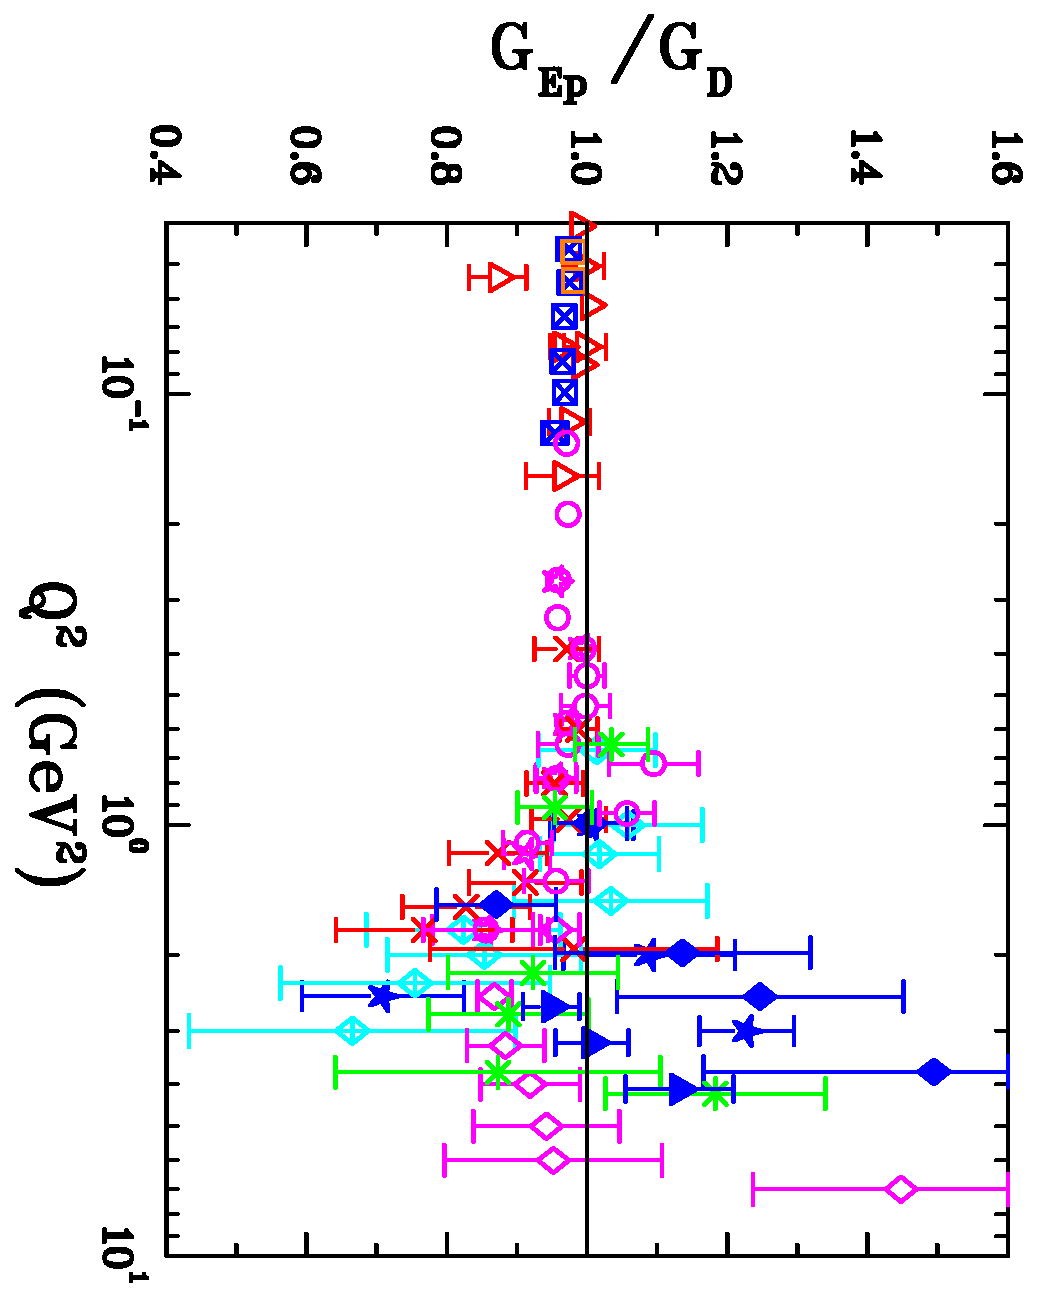
\includegraphics[angle=90]{gepgd_Dspin11.eps}
}
\caption{Q$^2$-dependence of the ratio $G_{Ep}/G_D$ obtained by the Rosenbluth separation method. $G_D$ is the dipole form factor. All data published after 1970 \cite{litt} are included}.
\label{fig:gepgd_cs}
\end{center}
\end{figure}

%%%%%%%%%%%%%%%%Fig 3
\begin{figure}
\begin{center}
\resizebox{0.485\textwidth}{!}{%
  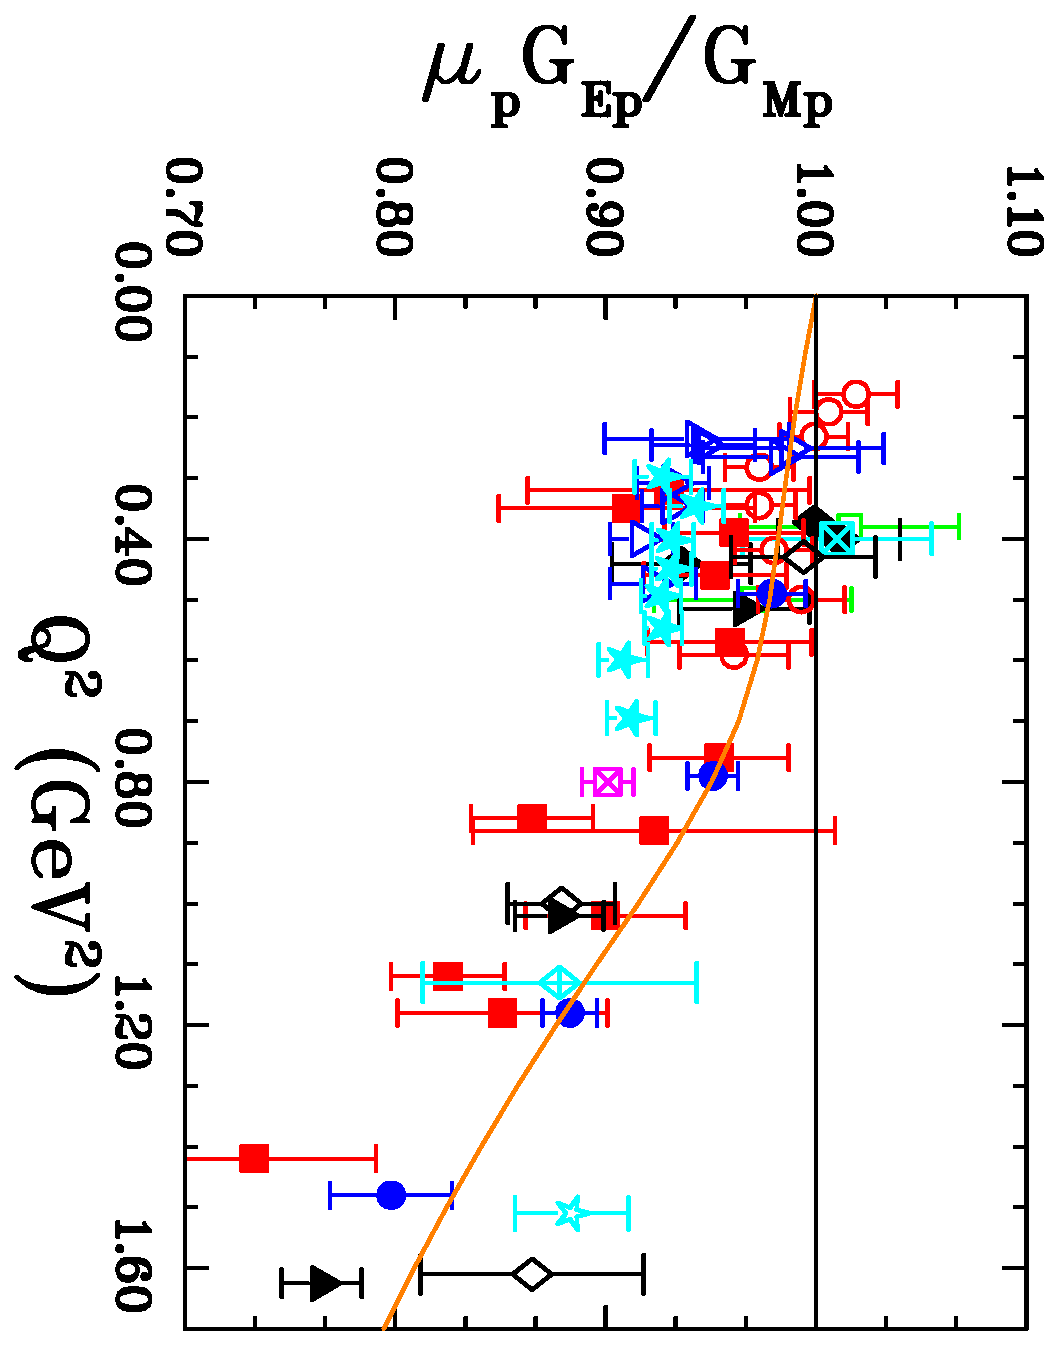
\includegraphics[angle=90]{gepgmp_low_nofit_10092014.eps}
}
\caption{Ratio $G_{Ep}G_{Mp}$ for $Q^2$ smaller than 1.5 GeV$^2$. The inconsistency of the various experiments are highlighted here.}
\label{fig:gepgd_cs}
\end{center}
\end{figure}

%%%%%%%%%%%%%%Figure 4
\begin{figure}
\begin{center}
\resizebox{0.485\textwidth}{!}{%
  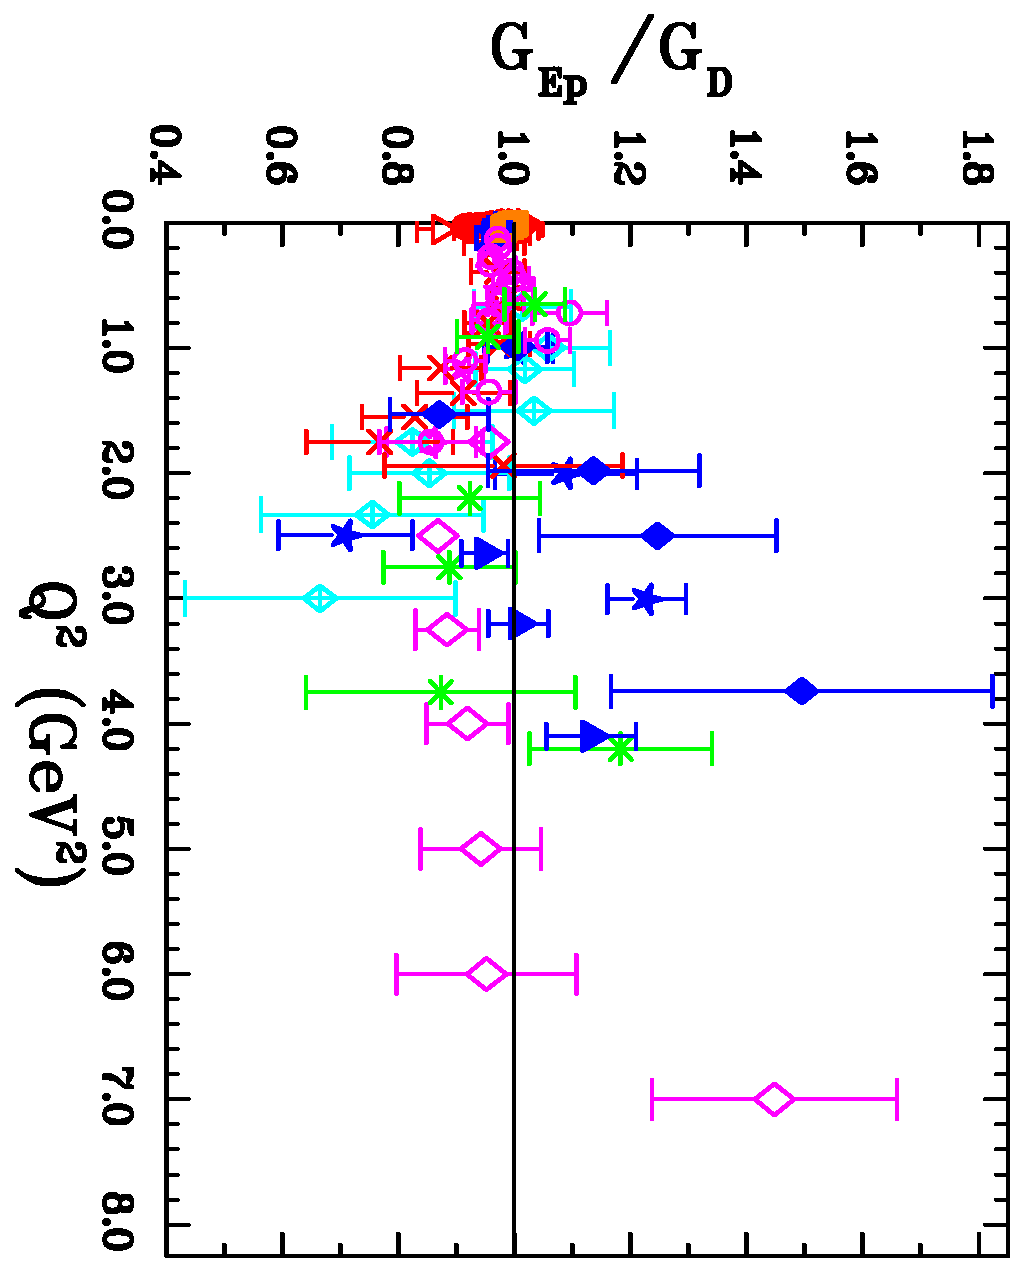
\includegraphics[angle=90]{gepgd_col_lininx.eps}
}
\caption{Ratio $G_{Ep}G_{Mp}$ from all Rosenbluth experiments on a linear scale in $Q^2$; to be compared with the same data displayed on a log scale.}
\label{fig:gepgd_lin}
\end{center}
\end{figure}

The modern version of the Rosenbluth separation technique takes advantage 
of the linear dependence in $\epsilon$, in the reduced 
cross section $\sigma_{red}$, based on Eq. (\ref{eq:csgegm}), as follows:
\begin{eqnarray}
\left(\frac{d\sigma}{d\Omega}\right)_{red} &=& \epsilon(1+\tau)\frac{E_{beam}}{E_e}\left(\frac{d\sigma}{d\Omega}\right)_{exp} / \left(\frac{d\sigma}{d\Omega}\right)_{Mott} \nonumber \\
&=& \tau G_{M}^2+\epsilon G_{E}^2,
\label{eq:redcs}
\end{eqnarray}
\noindent showing that the reduced cross section $\sigma_{red}$ is expected to have a linear dependence on $\epsilon$, with slope proportional 
to $G_{E}^2$ and intercept equal to $\tau G_{M}^2$. To illustrate the method, the reduced cross section data, $\sigma_{red}$, of ref. 
\cite{qattan05} are shown in Fig. \ref{fig:geplt1}. The 
corresponding form factor ratios are shown in Fig. \ref{fig:gepgd_cs} on a background of other form factor ratios obtained from Rosenbluth
separations. Also shown on this figure are the results of the first two recoil polarization experiments obtained in hall A, triangle symbols. 
\cite{jones,punjabi05A,punjabi05B,gayou:2002}. The dichotomy between cross section (Rosenbluth separation) and recoil polarization results is very obvious indeed from this figure.

\subsubsection{Proton Radius}

In a general sense the elastic {\it {ep}}  cross section is related to the Mott cross section for a spin $\frac{1}{2}$ electron
without internal structure times the Fourier transform of the charge and/or magnetization density of the target nucleon as follows:
\begin{equation}
\sigma(\theta_e)=\sigma_{Mott}\times\left|\int_{volume}\rho(\vec r)exp{i\vec{q}.\vec r}d^3\vec r\right|^2
\end{equation}    
\noindent where $\rho(\vec r)$ is either the electric- or the magnetic spacial distribution function. If follows, for the particular of 
the electric form factor G$_{Ep}(Q^2)$, that for short distances it can be expanded in terms of even moments of the distance $<r_e^{2n}>$ as:
\begin{equation}
G_{Ep}=1 - \frac{1}{6}{Q^2<r_e{^2}>} + \frac{1}{120}{Q^4<r_e{^4}>} ... 
\label{eq:rms}
\end{equation}
\noindent Hence for very small distance within the nucleon, the mean-square radius of the proton can be obtained from the derivative of
 Eq. \ref{eq:rms} 
\begin{equation}
\frac{dG_{Ep}}{dQ^2}=-\frac{1}{6}|left{r_e{^2}}|right_{at Q^2=0}
\end{equation}
\noindent from which follows the relation 
\begin{equation}
<r_e{^2}> = - 6|left\frac{dG_{Ep}}{dQ^2}|right_{at Q^2=0}; 
\end{equation}
A similar relation holds for the magnetic radius $<r_m{^2}>$.
Many electron scattering experiments have obtained values of $<r_e{^2}>$ by fitting low Q$^2$ cross section data \cite{sick:2003,sick:2014} ; 
$<r_m{^2}>$ is more difficult to obtain as its contribution to the cross section is weighted down by the factor $\tau$ (see Equ. \ref{eq:csgegm}). 

The proton radius can also be obtained from precise measurements of the Lamb shift energies either in the hydrogen atom 
(Ref. \cite{melnikov:2000}), or in muonic hydrogen (Ref. \cite{antognini:2013}). 
In both cases the 2S-2P Lamb shift is affected by the fact that the S-state wave function is maximum at the hydrogen's center,
 while the P-state has minimal overlap with the hydrogen nucleus. Recent measurements of the muonic Lamb shift energies at PSI have produced
values of $<r_e{^2}>$ which are smaller than the mean value of all electron scattering experiments by 7 $\sigma$ (\cite{pohl:2013}).  


\subsection{Formalism of double polarization experiments}

In 1968 and 1974 Akhiezer and Rekalo \cite{akh1A,akh1B} discussed the interest of measuring 
an interference term of the form  $G_{E}G_{M}$ by measuring the transverse 
component of the recoiling proton polarization in $\vec e p~\rightarrow~e \vec p$  
at large Q$^2$, to obtain $G_E$ in the presence of a dominating $G_M$.
In a review paper Dombey \cite{dombey} emphasized the virtues of measurements with a polarized lepton beam 
on a polarized target to obtain polarization observables. 
Also much later in 1982 Arnold, Carlson and Gross \cite{arnold} discussed in detail, that the best way 
to measure the neutron and proton form factors would be to use the $^2H( \vec e,e' \vec n)n$ 
and $^1H( \vec e,e' \vec p)$ reactions, respectively.

Indeed, both the recoil polarization and target asymmetry measurement methods have
been used successfully to measure the proton and neutron form factors to high 
four momentum transfer, $Q^2$, at Jefferson Lab. These methods have been used also at MIT-Bates, the Mainz 
Microtron (MAMI),and Nationaal Instituut voor Kernfysica en Hoge Energie Fysica (NIKHEF), to make precise 
proton and neutron form factor measurements at lower $Q^2$. Both methods are discussed below, with 
benefits and drawbacks of using polarized target and focal plane polarimeter.  


\subsubsection{Recoil polarization method}

\label{subsubsec:poltrans}

With a longitudinally polarized electron beam and an un-polarized hydrogen target, the 
polarization of the incoming electron is transferred to the proton via an exchange of a virtual photon as 
shown in Fig. \ref{fig:nlt}. 
For elastic ep 
scattering with a longitudinally polarized electron beam, the only non-zero
polarization transfer observables are the longitudinal and transverse
polarizations, $P_{\ell}$ and $P_t$. For single photon exchange, the 
transferred polarization can be written in terms of the Sachs form factors as:

\begin{eqnarray}
I_o P_n & = & 0  \nonumber \\
%I_oP_t & = & -hP_e2 \sqrt{\tau(1+\tau)}\tan\frac{\theta_e}{2} G_EG_M  \nonumber \\ 
I_oP_\ell & = & hP_e\frac{(E_{beam}+E_{e})}{M}\sqrt{\tau(1+\tau)}\tan^2\frac{\theta_e}{2}  G_M^2 \nonumber \\ 
I_oP_t & = & -hP_e2 \sqrt{\tau(1+\tau)}\tan\frac{\theta_e}{2} G_EG_M 
\end{eqnarray}

\noindent
where $h = \pm 1$ and $P_e$ are the beam helicity and polarization, respectively; $E_{beam}$ and $E_{e}$ are the incident and scattered 
electron energies, $\theta_{e}$ is the electron scattering angle, and M is the 
mass of the proton; $I_o=G_E^2+\frac{\tau}{\epsilon}G_M^2$, is the unpolarized cross section and 
$\epsilon=[1+2(1+\tau)\tan^2\frac{\theta_{e}}{2}]^{-1}$ is the longitudinal polarization of the virtual photon.


%%%%%%%%%%%%%%Figure 5 kinematics
\begin{figure}
\begin{center}
\resizebox{0.45\textwidth}{!}{%
\includegraphics{ep_recoilpol_10312014.eps}
}
\caption{Illustration of the kinematics and polarization of the recoil proton for $\vec e p\rightarrow e' \vec p$.}
\label{fig:nlt}
\end{center}
\end{figure}

The ratio of $G_E$ and $G_M$ is then directly obtained from the ratio of the two polarizations $P_t$ and $P_{\ell}$
components:
\begin{equation}
\frac{G_{E}}{G_{M}}=-\frac{P_{t}}{P_{\ell}}\frac{(E_{beam}+E_{e})} 
{2M}\tan (\frac{\theta_{e}}{2}).
\label{eq:ratio}
\end{equation}

In the one-photon exchange process, the form factors depend only on $Q^2$ and a deviation from constant would 
indicate a mechanism beyond the Born approximation. For each $Q^2$, a single measurement of the azimuthal angular
distribution of the proton scattered in a secondary target gives both the longitudinal and transverse polarizations.
Thus the ratio of electric to magnetic form factors of the proton is obtained directly from a simultaneous 
measurement of the two recoil polarization components. The knowledge of the beam polarization and of the analyzing power of the 
polarimeter is not needed to extract the ratio, $G_{E}/G_{M}$.  The kinematic factors in Eq. (\ref{eq:ratio}) are
typically known to a precision far greater than the statistical precision of the recoil polarization components.



\subsubsection{Asymmetry with polarized targets}
\label{subsubsec:Asymmetry}


It was discussed by Dombey \cite{dombey} in a review paper in 1969 that the nucleon form factors 
can be extracted from the scattering of longitudinally polarized electrons off
a polarized nucleon target. 
In the one photon exchange approximation, the elastic electron nucleon
scattering cross section can be written reaction en as a sum of two parts: $\Sigma$, which corresponds to
the unpolarized elastic differential cross section $d\sigma/d\Omega_e$, and a polarized part $\Delta$, which is
non-zero only if the electron beam is longitudinal polarized \cite{donnelly,raskin};

\begin{equation} 
\sigma_{h} = \Sigma + h \Delta, \\
\label{eq:asymm}
\end{equation}
\noindent
where h is the beam helicity, and $\Sigma$ the unpolarized elastic {\it {ep}} cross section can be written as:
\begin{equation} 
\Sigma =  \left(\frac{d\sigma}{d\Omega}\right)_{Mott}{\frac{E_e}{E_{beam}}}{\frac{1}{1+\tau}}\left[G_E^2 + \frac{\tau}{\epsilon}G_M^2 \right]. \\
\label{eq:Sigma}
\end{equation}

The polarized part of the cross section, $\Delta$, with two terms related to the directions of the target polarization, 
$\vec{P}(\theta^{\ast} \phi^{\ast})$, is given by \cite{donnelly,raskin}: 
\begin{eqnarray}
\Delta & = & -2 \left(\frac{d\sigma}{d\Omega}\right)_{Mott} \frac{E_e}{E_{beam}}\tan\frac{\theta_e}{2} \sqrt{\frac{\tau}{1+\tau}} \nonumber \\
& & \Big(\sqrt{\tau\big[1+(1+\tau)\tan^2\frac{\theta_e}{2}\big]} \cos\theta^{\ast}G_M^2  \nonumber \\
&+&\sin\theta^{\ast}\cos\phi^{\ast}G_E G_M  \Big)
\label{eq:delta}
\end{eqnarray}
\noindent
where $\theta^{\ast}$ and $\phi^{\ast}$ are the polar and 
azimuthal laboratory angles of the target polarization vector with $\vec q$ in the $\vec z$
direction and $\vec y$ normal to the electron scattering plane, as shown 
in Figure \ref{fig:epkin_asym}.

%%%%%%%%%%%%%Fig 6 kinematics
\begin{figure}
\begin{center}
\resizebox{0.45\textwidth}{!}{%
\includegraphics{ep_asymmetry_10312014.eps}
}
\caption{Illustration of the kinematics and orientation of the target polarization $\vec P$, for the reaction $\vec e \vec n \rightarrow e' n$. }
\label{fig:epkin_asym}
\end{center}
\end{figure}

The physical asymmetry $A$ is then defined as 
\begin{equation}
A=\frac{\sigma_{+} -\sigma_{-}}{\sigma_{+} + \sigma_{-}}=\frac{\Delta}{\Sigma},
\label{eq:asy}
\end{equation}
\noindent
where $\sigma_+$ and $\sigma_-$ are the cross sections for the two beam helicities. 

For a longitudinally polarized beam and polarized target, the measured asymmetry, $A_{meas}$, is 
related to the physical asymmetry, $A$, by 
\begin{equation}
A_{meas}=P_{beam}P_{target}A,
\label{eq:asy1}
\end{equation}
\noindent
where $P_{beam}$ and $P_{target}$ are electron beam and target polarization, respectively, and 
 $A$ can be obtained using Eqs. (\ref{eq:Sigma}) and (\ref{eq:delta}),  
\begin{eqnarray}
A &=&-\frac{2\sqrt{\tau(1+\tau)}\tan\frac{\theta_e}{2}}{G_E^2+\frac{\tau}{\epsilon}G_M^2}
\Big[ \sin\theta^{\ast}\cos\phi^{\ast}G_E G_M \nonumber \\
&+& \sqrt{\tau\big[1+(1+\tau)\tan^2\frac{\theta_e}{2}\big]} \cos\theta^{\ast}G_M^2 \Big].
\label{eq:asy2}
\end{eqnarray}

From Eq. (\ref{eq:asy2}), it is apparent that to extract $G_{E}$, the target polarization 
in the laboratory frame must be perpendicular with respect to the momentum transfer vector ${\vec q}$
and within the reaction plane, with $\theta^{\ast}= \pi/2$ and $\phi^{\ast}= 0^o$ or $180^o$. 
For these conditions, the physical asymmetry $A$ in Eq. (\ref{eq:asy2}) simplifies to:
\begin{equation}
A_{perp}=\frac{-2\sqrt{\tau(1+\tau)}\tan\frac{\theta_e}{2} \frac{G_E}{G_M}}{(\frac{G_E}{G_M})^2+\frac{\tau}{\epsilon}}.
\label{eq:asy3}
\end{equation}
\noindent
As $(G_E/G_M)^2$ is quite small, $A_{perp}$ is approximately proportional to $G_E/G_M$. In practice, the second term in 
Eq. (\ref{eq:asy2}) is not strictly zero due to the finite acceptance of the detectors, but these effects are small and depend
on kinematics only in first order and can be corrected for, so the ratio $G_E/G_M$ is not affected directly.

The discussion above is only applicable to a free electron-nucleon scattering. 
For a quasi-elastic electron scattering from a nuclear targets, like $^2$H or $^3$He, corrections are required for several nuclear effects. 

\subsection{Two-photon exchange}

In the one-photon exchange process, the form factors depend only on $Q^2$
and a deviation from constant would indicate a mechanism beyond
the Born approximation. 

In the general case, 
elastic $ep$ scattering can be described by three
complex amplitudes \cite{diehl:2013,guichon,afanbrod,kivel:2012}:  $\tilde{G}_M$, $\tilde{G}_E$,
and $\tilde{F}_3$, the first two 
chosen as generalizations of the Sachs 
electric and magnetic form factors, $G_E$ and $G_M$, and the 
last one, $\tilde{F}_3$, vanishing in case of Born approximation.
The reduced cross section, $\sigma _{red}$, and the
proton polarization transfer components $P_t$ and $P_{\ell}$,
including two-photon exchange formalism, can be written as \cite{guichon}:

\begin{eqnarray}
\sigma_{red}&=& G_M^2 + \frac{\varepsilon}{\tau}G_E^2 + 2 G_M\Re\left(\delta \tilde{G}_M + \frac{\varepsilon}{M^2} \tilde F_3\right) 
\nonumber \\
&+& 2\frac{\varepsilon}{\tau} G_E \Re \left(\delta\tilde G_E + \frac{\nu}{M^2}\tilde F_3\right)
\label{eq:siggen}
\end{eqnarray}
\vspace{-0.25in}
\noindent with 
\begin{eqnarray}
\nu=\frac{s-u}{4M^2}=\sqrt{\tau(1-\tau}\frac{1+\varepsilon}{1-\varepsilon}.
\label{eq:nu2gamma}
\end{eqnarray}
\vspace{-0.25in}
\begin{eqnarray}
&P_t&=-\sqrt{\frac{2\varepsilon(1-\varepsilon)}{\tau}} \frac{1}{\sigma _{red}}  \nonumber \\
& &\left(G_E G_M + G_E\Re(\delta \tilde{G}_M) + G_M\Re(\delta \tilde{G}_E+\frac{\nu}{M^2}) \tilde F_3))\right)\nonumber\\
\label{eq:ptgen}
\end{eqnarray}
\vspace{-0.5in}
\begin{eqnarray}
&P_{\ell}&=\sqrt{(1-\varepsilon ^2)}\frac{1}{\sigma _{red}} \nonumber \\
& &\left(G_M^2 + +2 G_M \Re(\delta \tilde G_M+\frac{\epsilon}{1+\epsilon}\frac{\nu}{M^2}\tilde F3)\right)
\label{eq:plgen}
\mbox{,}
\end{eqnarray}
\vspace{-0.25in}
\\
%\begin{eqnarray}
%\frac{\sigma _{red}}{G_M^2}&=& 1+\frac{\varepsilon R^2}{\tau }+2\frac{\Re\delta \tilde{G}_M}{G_M} \nonumber \\
%&+& 2R\varepsilon \frac{\Re\delta \tilde{G}_E}{\tau G_M}+ 2\left(1+\frac{R}{\tau }\right){ \varepsilon Y_{2\gamma }}
%\label{eq:siggen}
\\
%P_t&=&-\sqrt{\frac{2\varepsilon(1-\varepsilon)}{\tau}}
%\frac{G_M^2}{\sigma _{red}}  \nonumber \\
%& &\left(R+
%R\frac{ \Re\delta \tilde{G}_M}{G_M}
%+\frac{ \Re\delta \tilde{G}_E}{G_M}
%+{ Y_{2\gamma }}\right)
%\label{eq:ptgen}
%\\
%P_l&=&\sqrt{(1-\varepsilon ^2)}\frac{G_M^2}{\sigma _{red}} \nonumber \\
%& &\left(1+2\frac{ \Re\delta \tilde{G}_M}{G_M}+\frac{2}{1+\varepsilon }{ \varepsilon Y_{2\gamma }}\right)  %\vspace{0.25in}
%\label{eq:plgen}
%\mbox{,}
%\end{eqnarray}
where:
\begin{eqnarray}
\Re\tilde{G_M}(Q^2,\varepsilon)&=&G_M(Q^2)+\Re\delta \tilde{G_M}(Q^2,\varepsilon)  \\ 
\label{eq:regm}
\Re\tilde{G_E}(Q^2,\varepsilon)&=&G_E(Q^2)+\Re\delta \tilde{G_E}(Q^2, \varepsilon) 
\label{eq:rege} 
\end{eqnarray}

Here $\tau=Q^{2}/4M_{p}^{2}$, 
and $\varepsilon =[1+2(1+\tau)\tan^2\frac{\theta_e}{2}]^{-1}$,
where  $\theta_e$ is the lab electron scattering angle.
While the Sachs form factors depend only on $Q^2$, in the general case the
amplitudes depend also on $\varepsilon$.
%The $Y_{2\gamma}$ function defined above is
%related to the third amplitude $\tilde{F}_3$. 
The  reduced cross section
and the transferred proton polarization components are sensitive only to the real part
of the amplitudes. 

In Born approximation only the first term remains in the reduced cross 
section, $\sigma _{red}$, and the
proton polarization transfer components $P_t$ and $P_l$ are :
\begin{eqnarray}
{\sigma _{red}}&=& G_M^2 + \frac{\varepsilon}{\tau }G_E^2
\label{eq:sigborn}
\\
P_t&=&-\sqrt{\frac{2\varepsilon(1-\varepsilon)}{\tau}} \frac{G_EG_M}{\sigma _{red}}
\label{eq:ptgen}
\mbox{,}  \\
%\; \; \;
P_{\ell}&=&\sqrt{(1-\varepsilon ^2)} \frac{G_M^2}{\sigma _{red}}
\label{eq:pborn}
%\label{eq:plborn}
\end{eqnarray}

\section{Recent developments; to be relocated}

The experimental and theoretical situation for the nucleon form factors were reviewed extensively in the 7 years following
publication of the results of the first recoil polarization experiment at Jefferson Lab \cite{jones}. Chronologically
these reviews include Gao \cite{gaoA,gaoB}, Hyde-Wright et al. \cite{charleskees}, Perdrisat et al. \cite{perdrisat:2006} and 
Arrington et al. \cite{arrreview}, Arrington et al \cite{arrington:2011}, Cloet et al. \cite{cloet:2008}
and Perdrisat and Punjabi \cite{scholar}. At this point in time, the double-polarization method had been used up to 5.6 GeV$^2$
for the proton form factor ratio $G_{Ep}/G_{Mp}$ (\cite{jones,punjabi05A,punjabi05B,gayou:2001}, and 1.45 GeV$^2$ for $G_{En}/G_{Mn}$. 
Recent polarization experiments at JLab for $G_{Mn}$ to a Q$^2$ of 0.6 GeV$^2$ \cite{anderson} had been published, and a 
mix of polarization and cross section had been obtained up to 5 GeV$^2$ for $G_{Mn}$, the latest  using the cross section
ratio method, to obtain $G_{Mn}$ from the measured 
${\frac{\frac{d\sigma}{d\Omega}[^2H(e,e'n)_{QE}]}{\frac{d\sigma}{d\Omega}[^2H(e,e'p)_{QE}]}}$ ratio \cite{brooksA,brooksB}.

The principal revelation coming out of the first $G_{Ep}/G_{Mp}$ experiment using recoil polarization was the systematic
decrease of this ratio with increasing Q$^2$. There existed data from the 1970's which suggested a similar behavior, 
although they were limited to Q$^2$ smaller than 3 GeV$^2$, and had large uncertainties. Interestingly, at that time, 
models based on vector meson dominance (VMD) \cite{iachello,hohler,gariA,gariB} were predicting a rapid decrease of the ratio
 $G_{Ep}/G_D$, reaching a value of 0.5 at Q$^2$ of 4 GeV/c. In the same period, a first paper from the Stanford group
\cite{litt} suggested a drastically different Q$^2$ dependence of the same ratio, $G_{Ep}/G_{Mp}$, with values reaching
1.35+/-0.3 at Q$^2$=3.6 GeV$^2$ (verify these numbers). The complete set of experimental results derived from cross 
section measurements is shown in Fig. \ref{fig:gepgd_cs} and \ref{fig:gmpgd_cs}. It includes the most recent JLab results
 of \cite{christy,qattan05}.

%%%%%%%%%%%%%%%%%%%%%%%%%%Figure 7
\begin{figure}
\begin{center}
\resizebox{0.45\textwidth}{!}{%
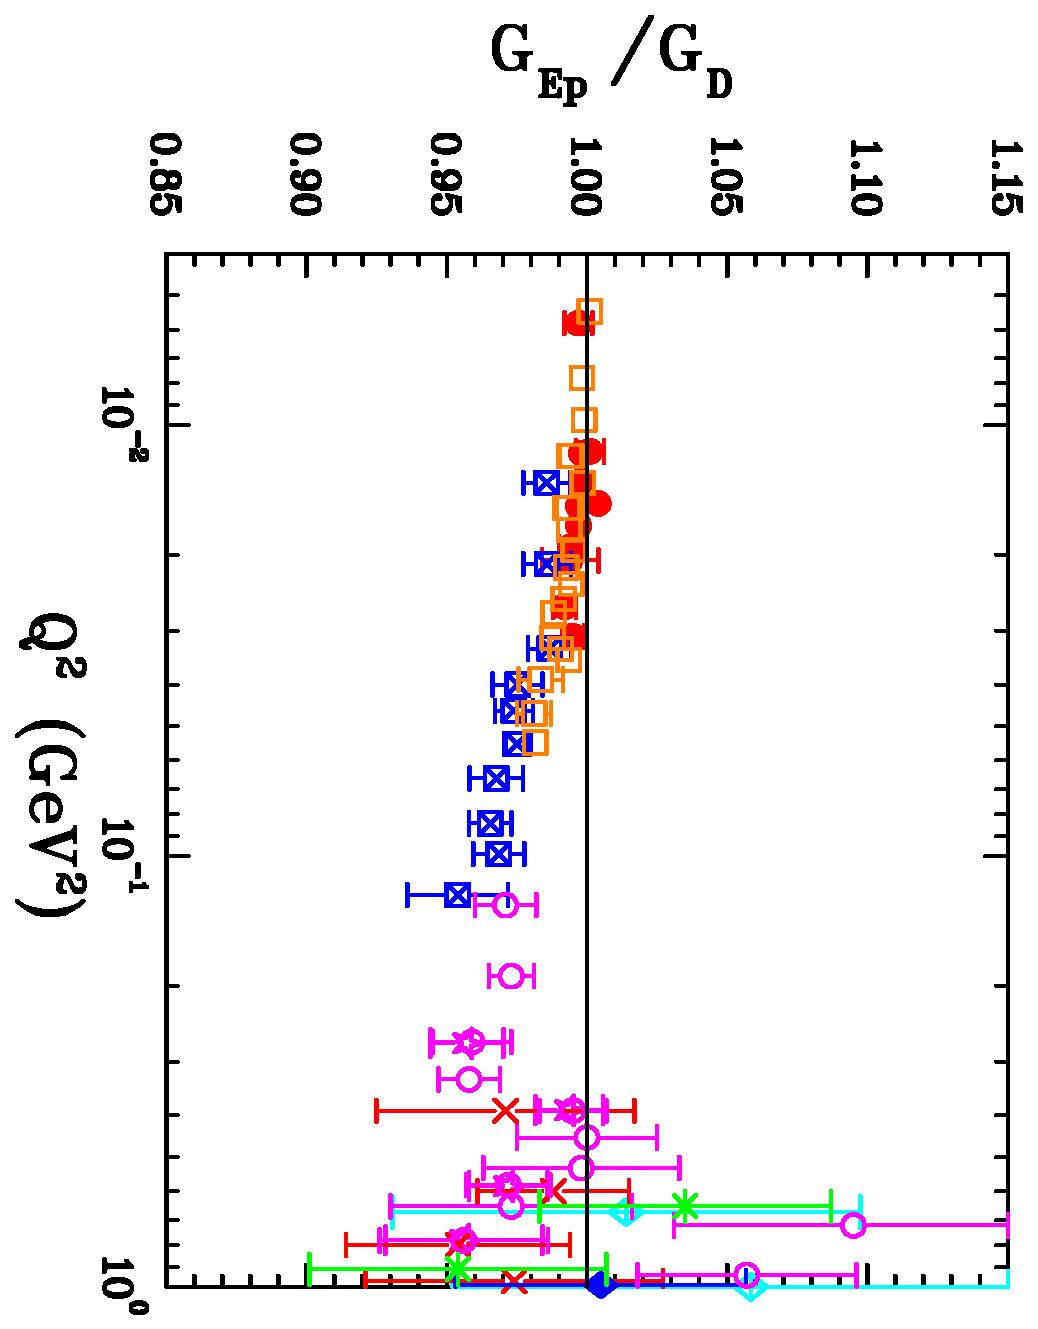
\includegraphics[angle=90]{gepgd_col_log_xmax1.eps}
}
\caption{Low $Q^2$ behavior of the $G_{Rp}/G_D$ ratio for Q$^2$ smaller than 1 GeV$^2$ for Rosenbluth data, illustrating the very small deviation from a constant of this ratio for small $Q^2$.}
\label{fig:gepgd}
\end{center}
\end{figure}

%%%%%%%%%%%%%%%%%% Figure 8
\begin{figure}
\begin{center}
\resizebox{0.45\textwidth}{!}{%
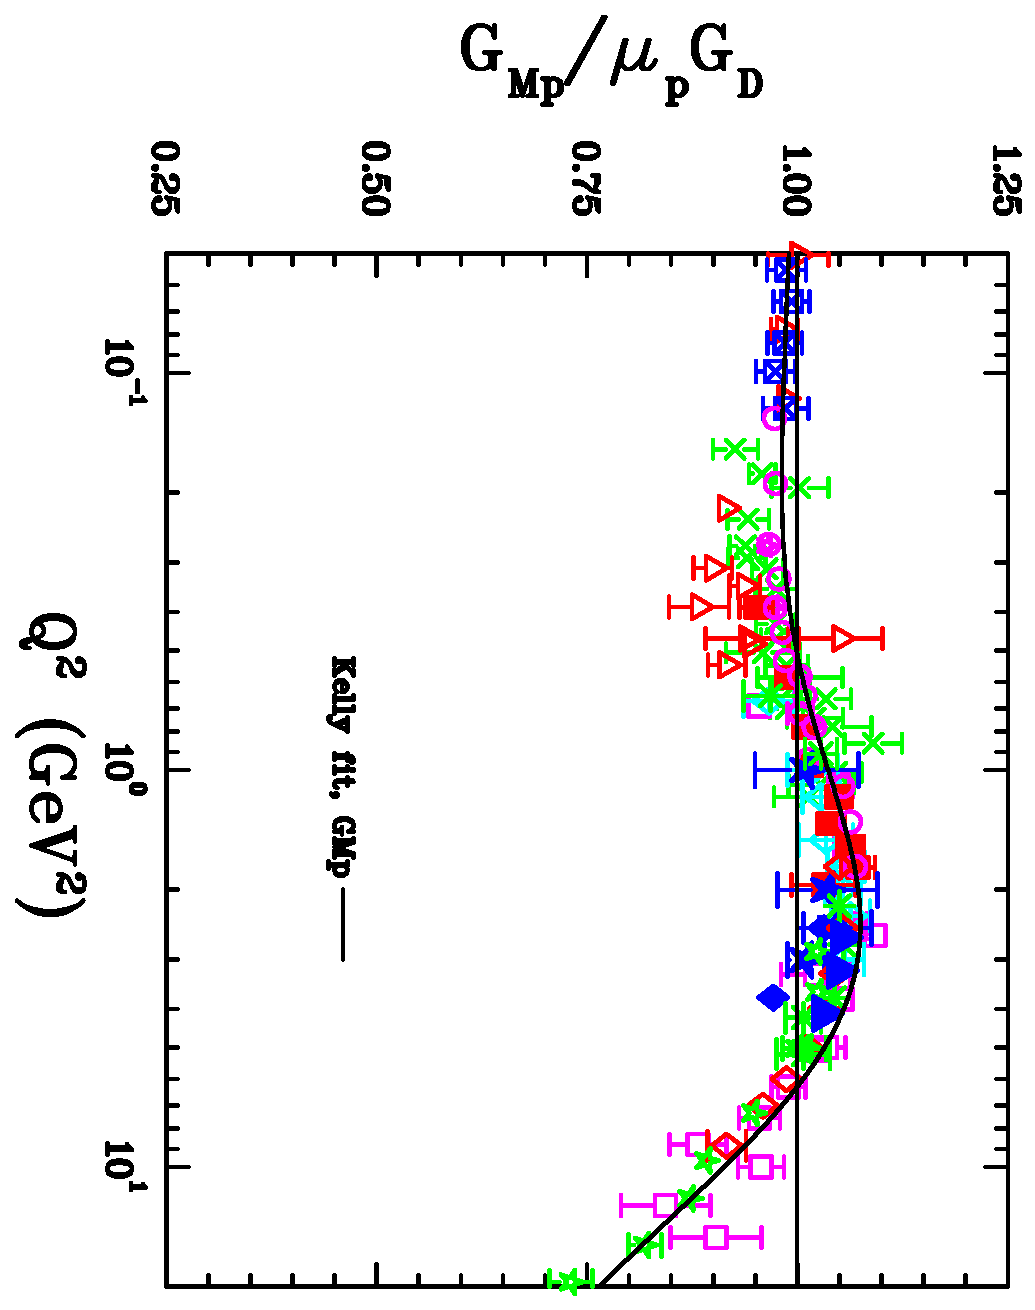
\includegraphics[angle=90]{gmpgd_spS.eps}
}
\caption{Rosenbluth values of $G_{Mp}/\mu_pG_D$ including all published data, for comparison with Fig. \ref{fig:geplt1}.} 
\label{fig:gmpgd_cs}
\end{center}
\end{figure} 

Since the last review paper was published, considerable theoretical work was performed. Some of the original models
discussed in the 1970's, in particular the original Vector Dominance (VMD), as well as the Constituent Quark
(CQM) models were revisited, made relativistic, then more of less left the front row, with the exception of 
Lomon \cite{lomon}, Bijker \cite{bijker} and others.

The proton form factors were originally introduced in non-relativistic scattering, as the three-dimensional Fourier
transform of the charge density \cite{hofs53,wilsonrr}. However the proton recoil implies that the electron
 is interacting with a moving charge distribution. Already for Q$^2$=0.25 GeV$^2$, the recoil proton relativistic 
boost factor $\gamma$ is 1.1, corresponding to $v/c=0.41$.
The argument that form factors are Fourier transforms of nucleon density in the Breit frame was abandoned, as this 
frame's velocity in the Lab frame is different for every Q$^2$.

The proton in its ground state is not necessarily spherically symmetric, but can show a typical multipole shape, 
when referred to the spin direction of one of its quarks (constituents) relative to the nucleon spin orientation
 \cite{miller:2003}. %shape of the proton

The wave front or infinite momentum frame densities are invariant, two-dimensional transverse charge and magnetization distribution, 
and are drastically different
from the non-relativistic ones \cite{miller:2003,carlson:2007}. % transverse densities in imf

Elastic ep scattering in the 1 to 10 GeV$^2$ range of 4-momentum squared transfer is
the domain of non-perturbative quantum chromodynamics (QCD); as a consequence of Dynamical Chiral Symmetry
Breaking, valence quarks acquire a mass of order $M_p/3$ in the infrared limit. \cite{cloet:2008b,cloet:2008}

   Scaling as a consequence of Perturbative QCD may have visible consequences even in the non-perturbative
 domain \cite{Galynskii:2013} 

The di-quark structure of the nucleon has observable consequences \cite{cloet:2012cy}

The mass of the dressed quarks originates from the QCD vacuum; it results
from accretion of quark-antiquark pairs from decaying gluons spontaneously emerging from the vacuum \cite{cloet:2008}. 

Assuming isospin symmetry one can obtain flavor separated dressed quark form
factors from simple linear relations between the Dirac and Pauli form factors.
The dressed up and down quarks have significantly different form factors 
\cite{cloet:2008,cates:2011,rohrmoser:2011,wilson:2011,Cloet:2013gva,qattan:2013}. 

A zero crossing of GEp, if and when observed,  would provide information on the dressed-quark mass
function \cite{diehl:2013}.

Nucleon form factors determine the parameters of the valence quark GPDs;
these can be used to obtain corresponding valence quark densities \cite{diehl:2013}.

The available data suggest that the isovector electric form factor (GEp-GEn) has a zero near $Q^2$~ 4.3 GeV$^2$;
this feature can be predicted in lattice calculations, from the connected diagram only. \cite{diehl:2013}.
 
Soft  Collinear Effective Theory (SCET), Kivel and Vanderhaeghen(2013)
for two-photon exchange \cite{kivel:2012}.

\section{GEn; to be relocated}

This in preparation  for the neutron section, in particular fig with $\mu_nG_{En}/G_{Mn}$. Nov. 3/14.

%%%%%%%%%%%%%%%%%%% Figure 9
\begin{figure}
\begin{center}
\resizebox{0.45\textwidth}{!}{%
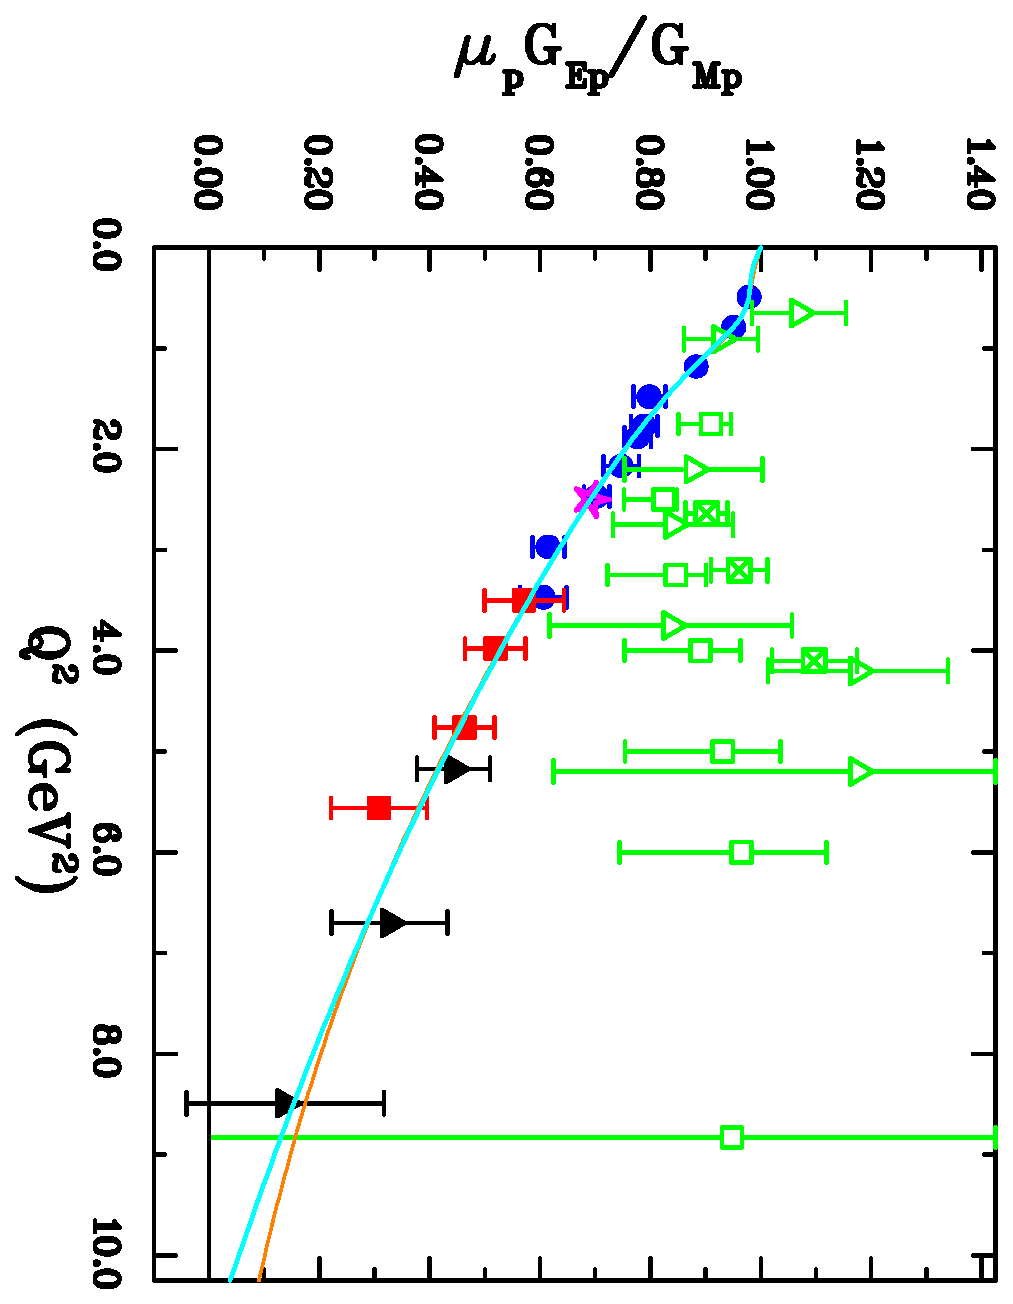
\includegraphics[angle=90]{gepgmp_allpol_allcs_noth_11072014.eps}
}
\caption{All data for the ratio $G_{Ep}/G_{Mp}$ obtained from the three large $Q^2$ recoil polarization experiments at JLab. Both curves are Kelly-type polynomial fits. The orange curve is a 7 parameter 
fit constrained with $\frac{1}{Q^2}$ asymptotic behavior. The azur curve a 6 parameter fits with constant asymptotic behavior.}
 
\label{fig:gepgmp}
\end{center}
\end{figure}

%%%%%%%%%%%%%%%%%%%Figure 10
\begin{figure}
\begin{center}
\resizebox{0.45\textwidth}{!}{%
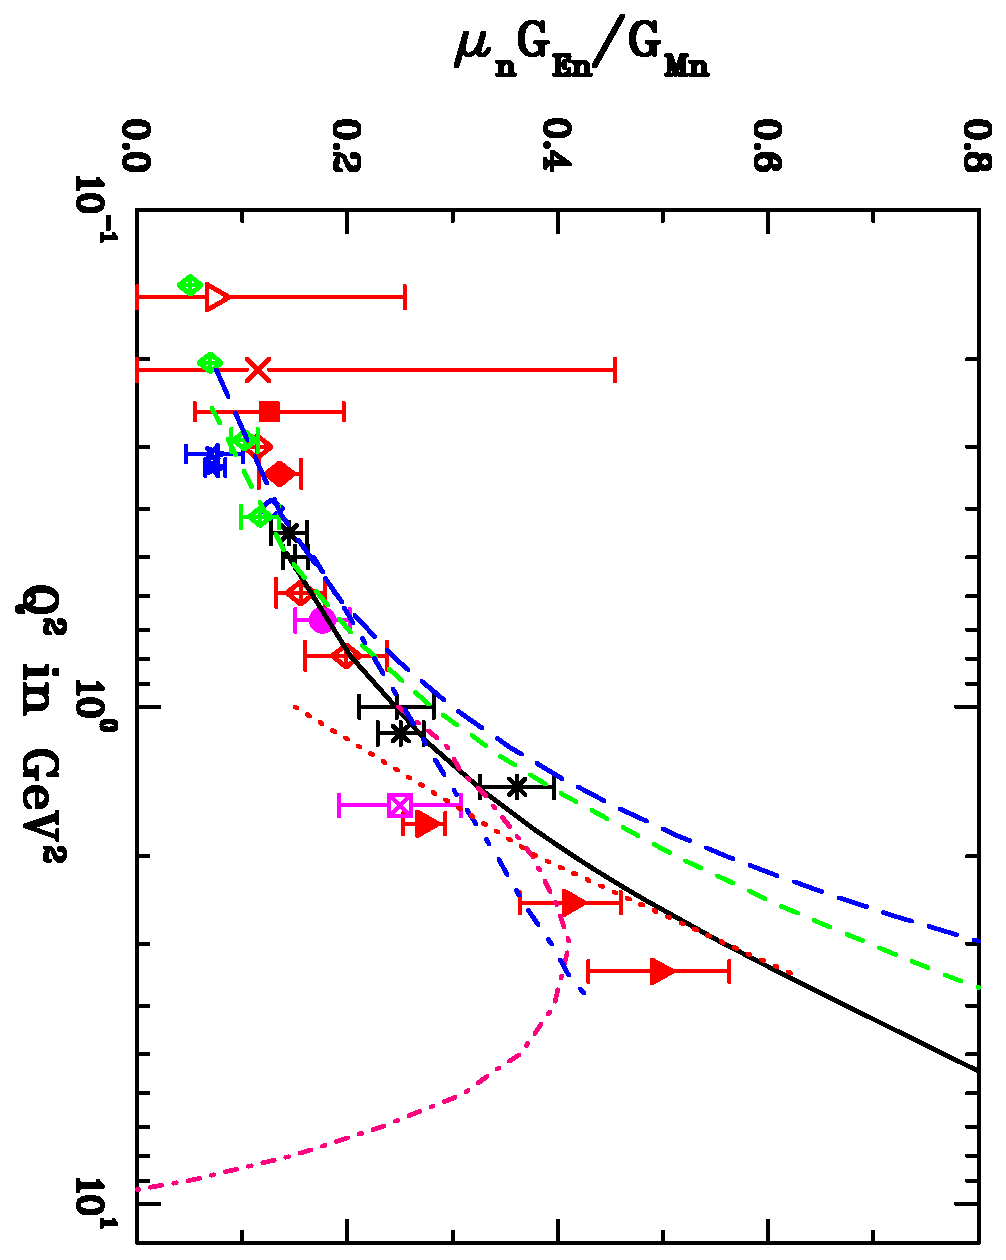
\includegraphics[angle=90]{gengmn_epja_nolbl_10302014.eps}
}
\caption{The complete data base for $G_{En}/G_{Mn}$ from double polarization experiments. Asymmetry with polarized D2 target: \cite{passchier,zhu,warren,geis:2008}, asymmetry with polarized $^3He$ target: \cite{cejones,thompson,meyerhoff:1994,becker,rohe,bermuth,golak:2001,riordan:2010,schlimme:2013}, recoil polarization with D2 target \cite{eden:1994,herberg,ostrick,glazier:2004,madey,plaster}}
\label{fig:neutron2}
\end{center}
\end{figure}

%%%%%%%%%%%%%%%%Figure 11
\begin{figure}
\begin{center}
\resizebox{0.45\textwidth}{!}{%
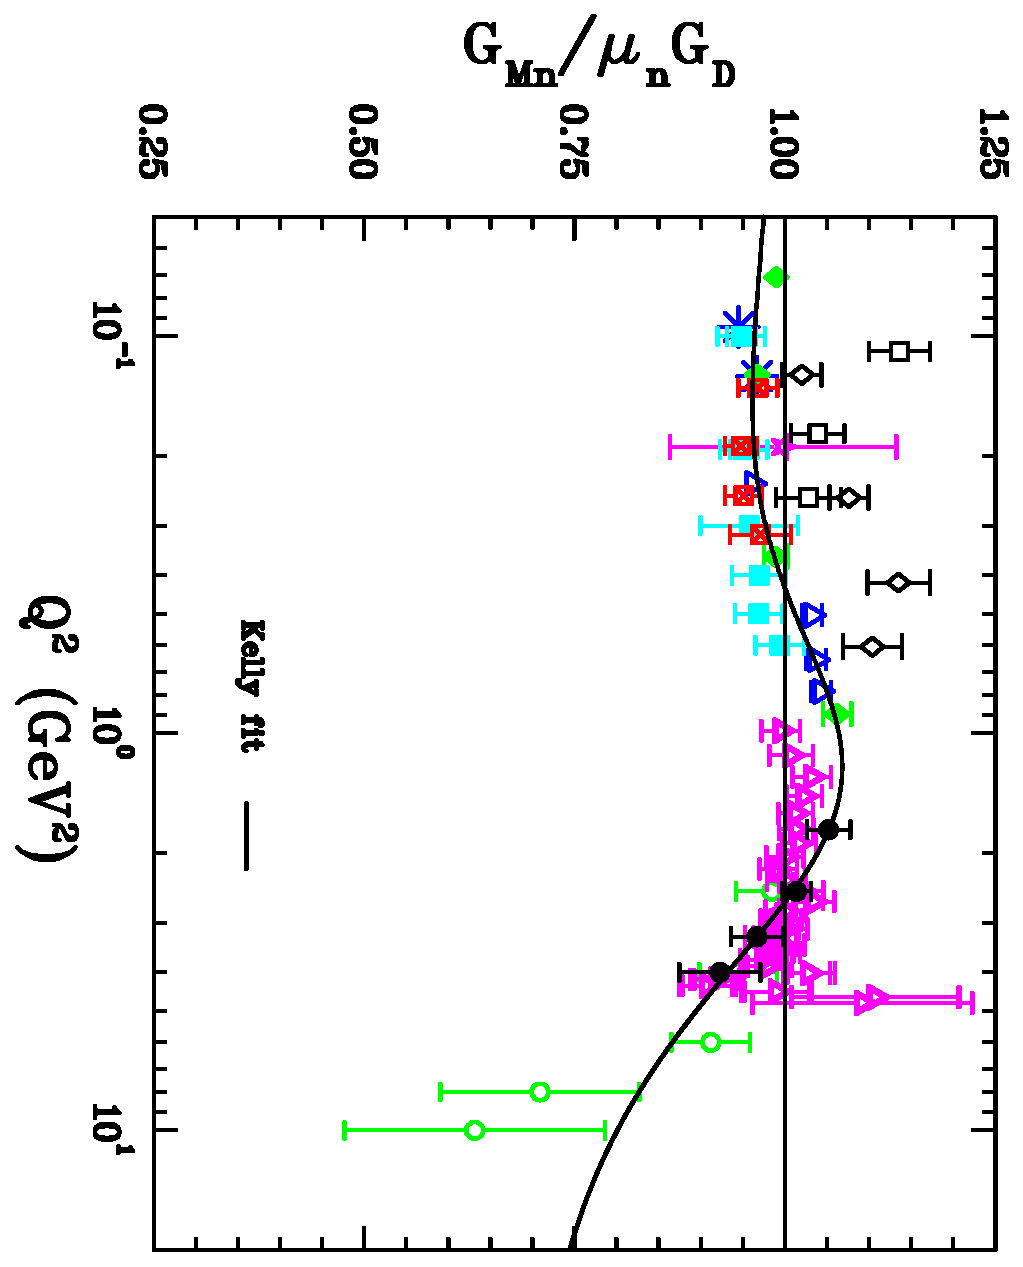
\includegraphics[angle=90.0]{gmngd_log.eps}
}
\caption{The complete data base for $G_{Mn}/\mu_nG_D$. May compare with the equivalent figure for $G_{Mp}/\mu_pG_D$ .}
\label{fig:gmn}
\end{center}
\end{figure}

\section{More Figures}

%%%%%%%%%%%%%%%%%%%%%%%%%%%% Figure 12
\begin{figure}
\begin{center}
\resizebox{0.45\textwidth}{!}{%
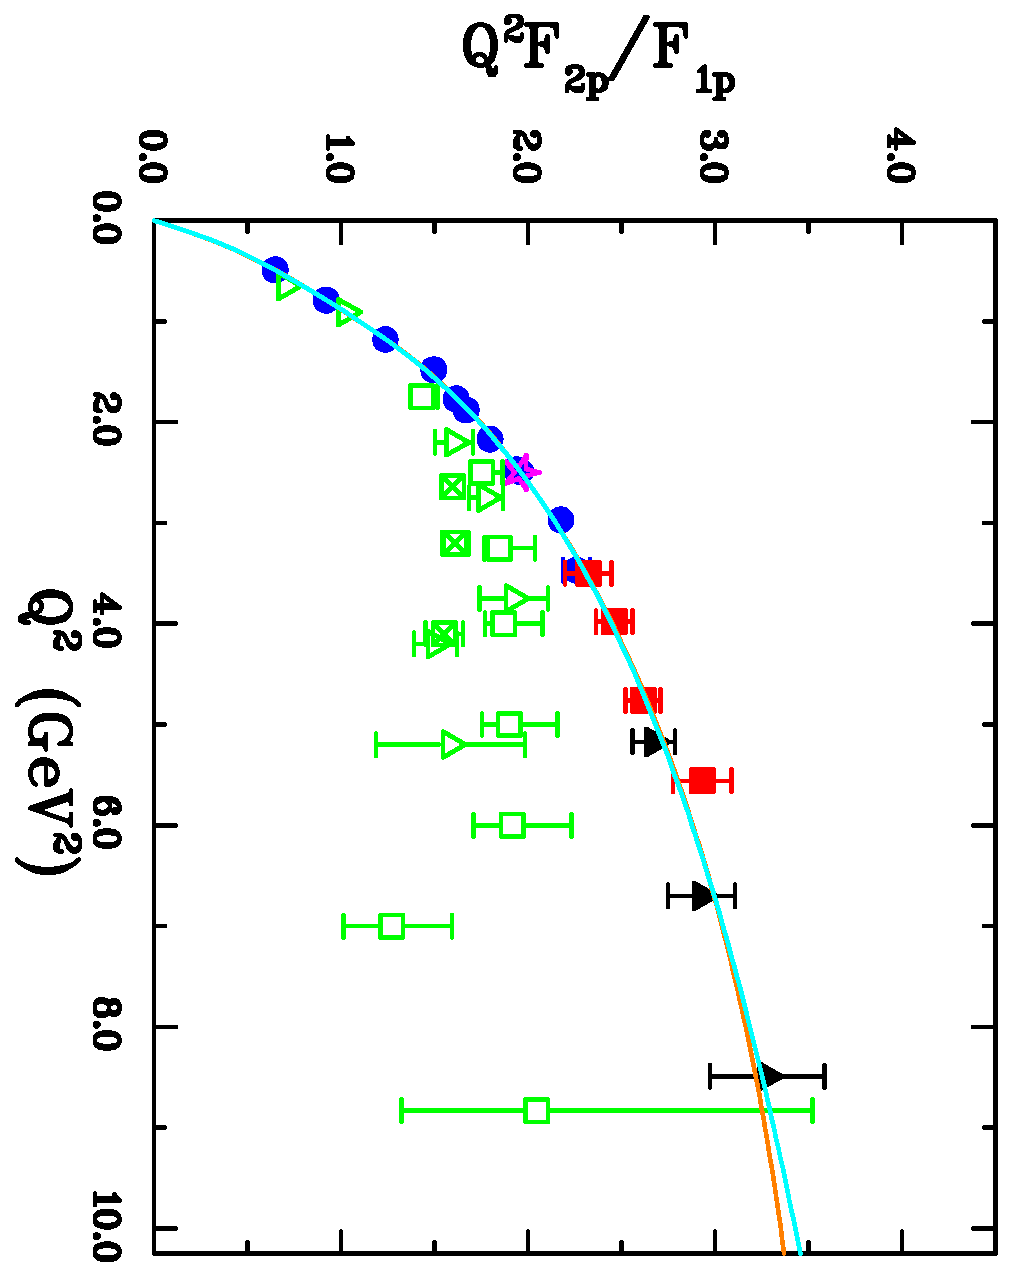
\includegraphics[angle=90]{q2f2f1_allpol_11072014.eps}
}
\caption{Behavior of the ratio $Q^2F_2/F_1$ for the proton, versus $^2$. JLab data for recoil polarization; empty symbols for Rosenbluth data. }.
\label{fig:q2f2f1p}
\end{center}
\end{figure}

%%%%%%%%%%%%%%%%%%%%%%%%%  Figure 13
\begin{figure}
\begin{center}
\resizebox{0.45\textwidth}{!}{%
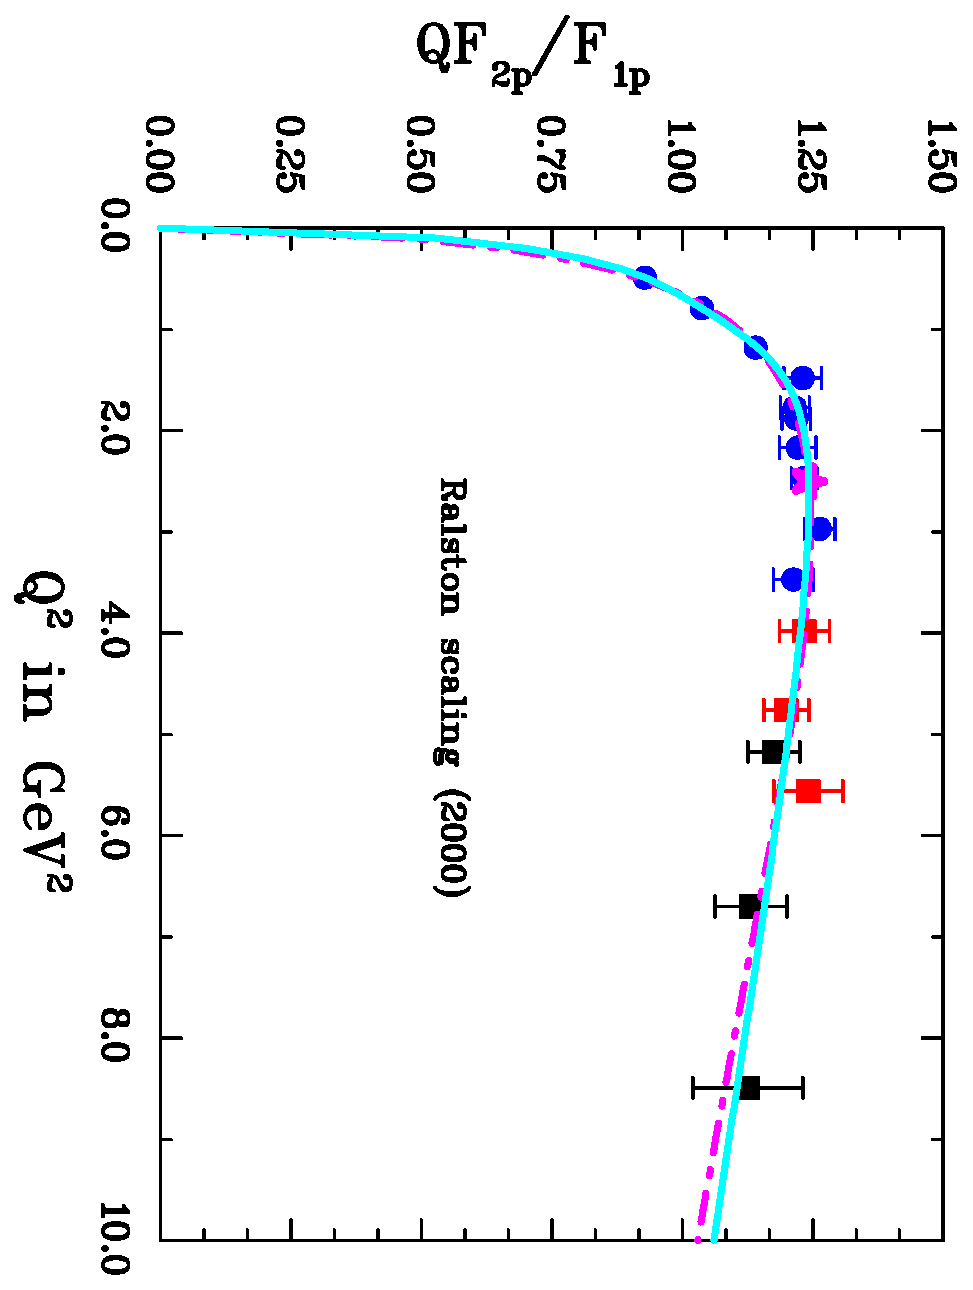
\includegraphics[angle=90]{qf2f1_gep3_colss.eps}
}
\caption{Behavior of the ratio $QF_2.F_1$ for the proton, as discussed by Ralston, \cite{jain}.}
\label{fig:pf2f1p}
\end{center}
\end{figure}

%%%%%%%%%%%%%%  Figure 14
\begin{figure}
\begin{center}
\resizebox{0.45\textwidth}{!}{%
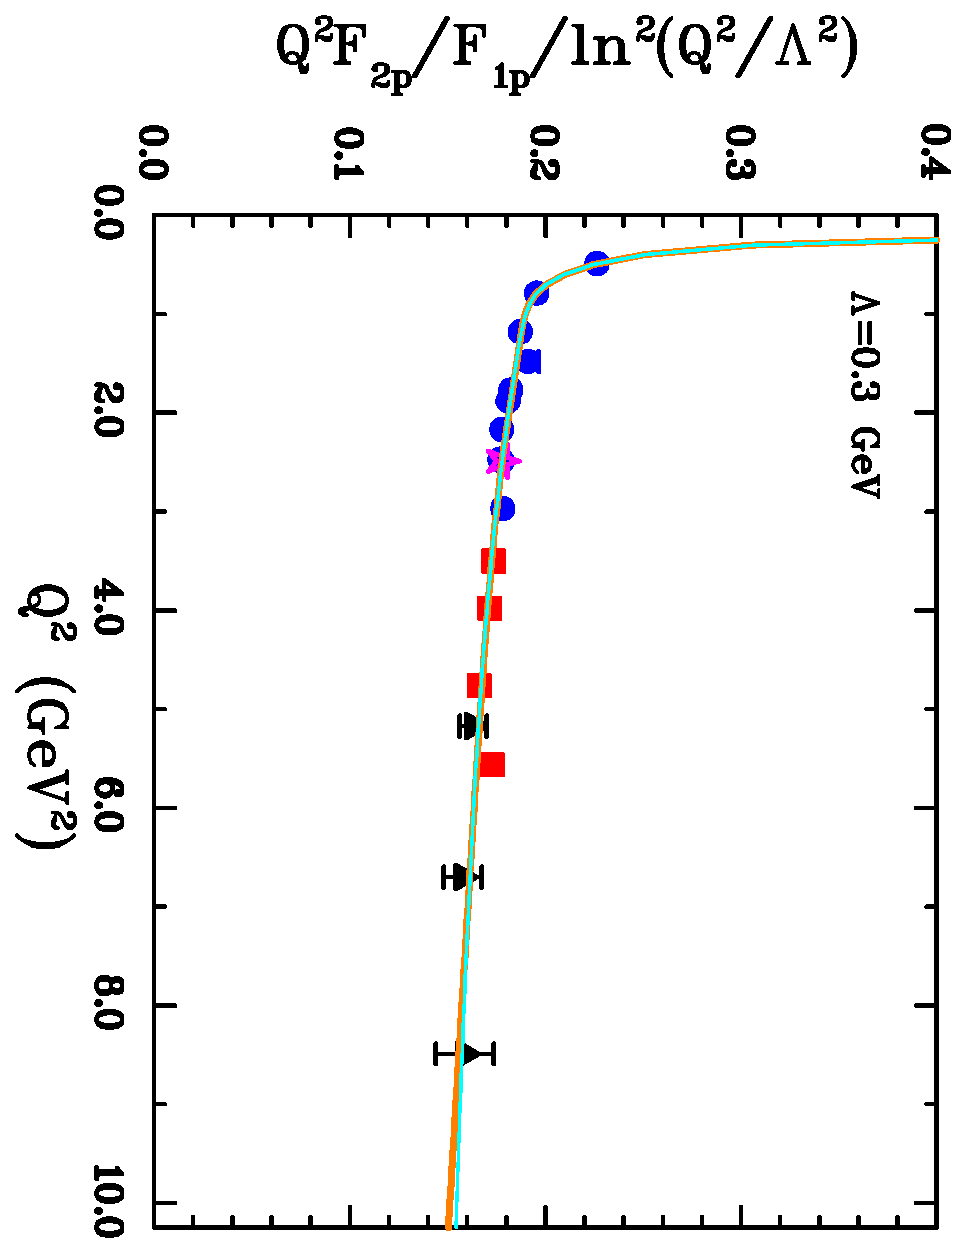
\includegraphics[angle=90]{q2f2f1_belitsky_nothss.eps}
}
\caption{Behavior of $Q^2F_2/F_1/ln^2(Q^2/\Lambda^2)$ as discussed by Belitsky \cite{belitsky:2002}.}
\label{fig:q2f2f1p}
\end{center}

\end{figure}

%%%%%%%%%%%%%%%%%%% Figure 15
\begin{figure}
\begin{center}
\resizebox{0.45\textwidth}{!}{%
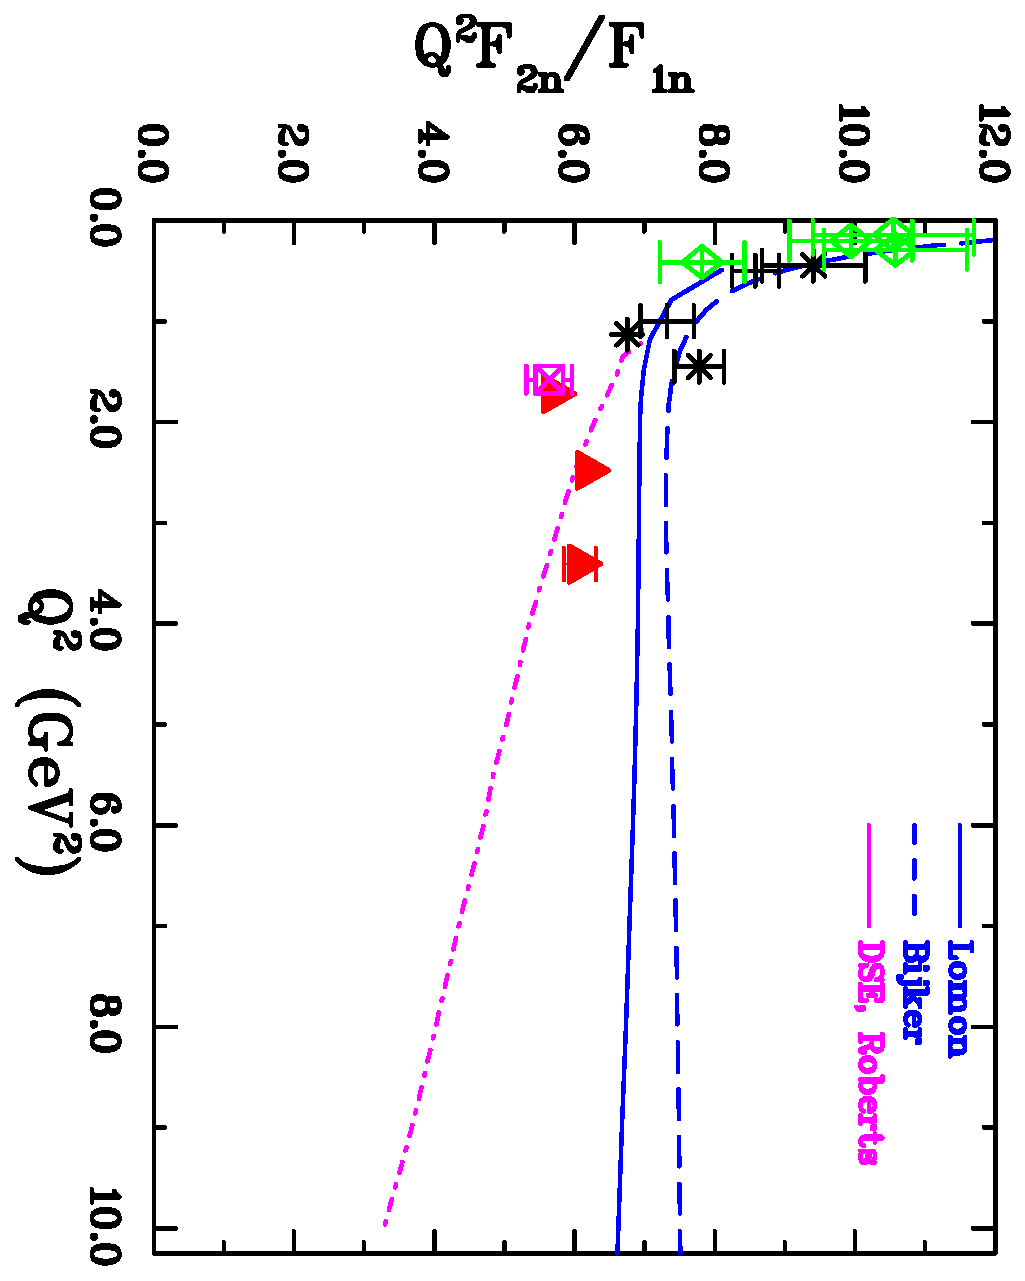
\includegraphics[angle=90]{q2f2f1_neutron_112311.eps}
}
\caption{Illustration of the current status on the asymptotic behavior of $Q^2F_2/F_1$ for the neutron; all data ;points from double polarization experiments. ``My Fit'' needs to be verified.}
\label{fig:pf2f1p}
\end{center}
\end{figure}

%%%%%%%%%%%%%%%%%%% Figure 16
\begin{figure}
\begin{center}
\resizebox{0.45\textwidth}{!}{%
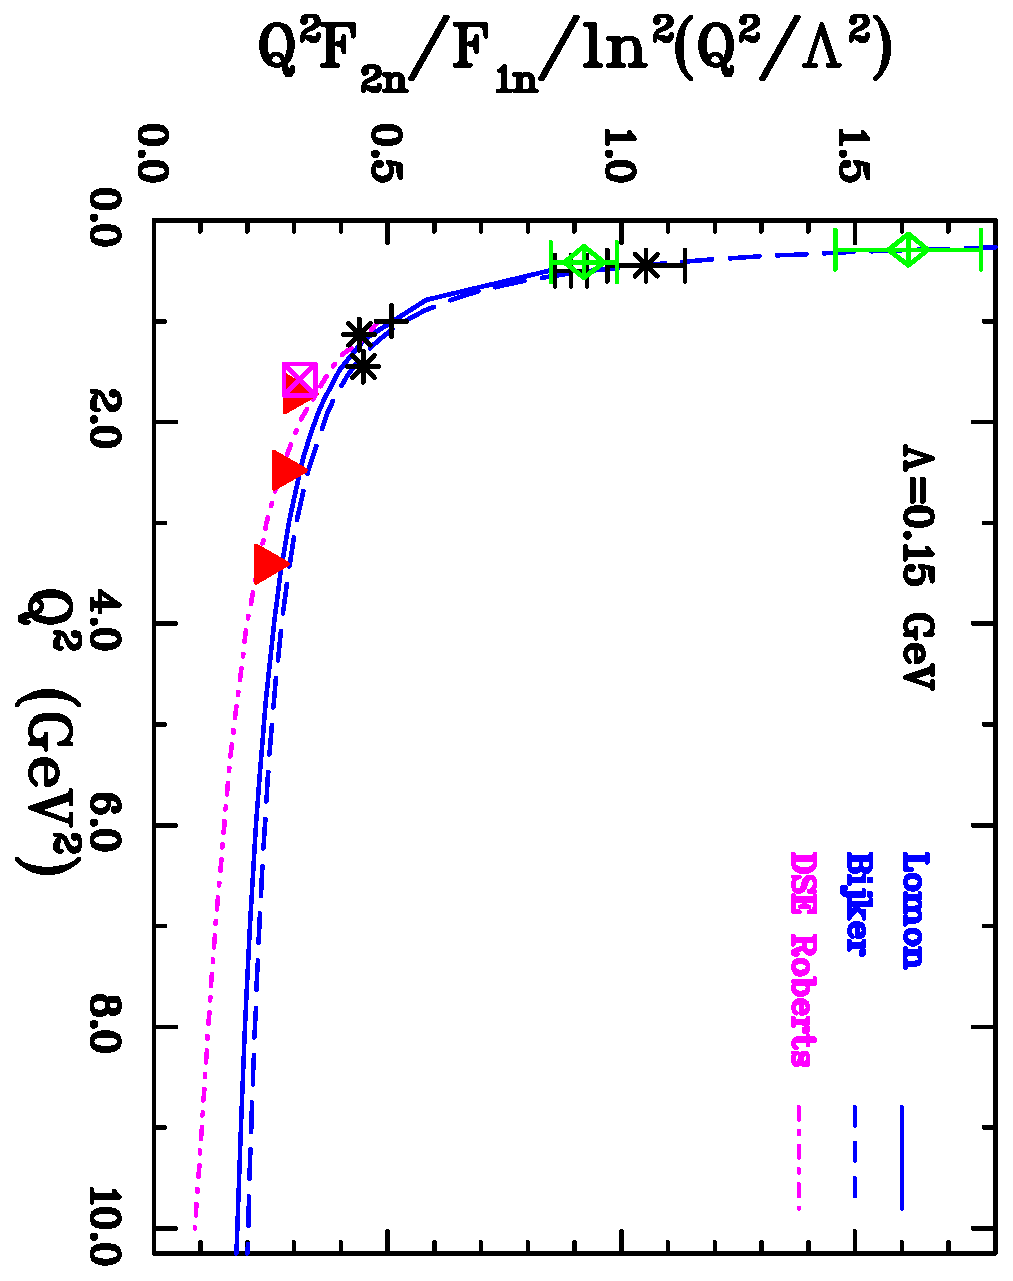
\includegraphics[angle=90]{q2f2f1_neutron_belitzky_052212.eps}
}
\caption{The Belitzky plot for the neutron}
\label{fig:nq2f2bel}
\end{center}
\end{figure}

%%%%%%%%%%%%%%added November 17, 2014

\section{Asymptotic behavior}

In the pQCD approach proposed by Brodsky and collaborators\cite{brodsky,brodlep}, 
the interaction is described as a convolution 
of a hard scattering amplitude and a baryon distribution amplitude. Up to
leading order in 1/$Q^2$, the magnetic form factor is proportional to 
$\alpha_s/Q^4$ times slowly varying logarithmic terms, because the momentum of the virtual
photon absorbed by one quark, must be shared with the two other quarks through the exchange of
two gluons. In lowest order the absorbed virtual photon cannot induce a quark helicity flip and 
consequently pQCD predicts a faster decrease of $F_{2p}$ 
than of $F_{1p}$ with increasing $Q^2$, by a factor $Q^{-2}$ \cite{brodsky}. 
The expectation is then that $Q^2 F_{2p}/F_{1p}$ should
become constant at very high $Q^2$. 
In Fig.~\ref{fig:q2f2f1} the JLab data together with data of Andivahis {\it et al.}\cite{andivahisA,andivahisB},
are shown as $Q^2 F_{2p}/F_{1p}$. The data from Ref. \cite{andivahisA,andivahisB} show flattening 
above $Q^2$ of 3 GeV$^2$. However, the data from this experiment do not show yet the specific pQCD $Q^2$ dependence.

Recently there have been  two revisions of the pQCD prediction
for the large $Q^2$ behavior of $F_2$. In the first, Brodsky \cite{Brodsky:2002} argues 
that the pQCD motivated behavior of $F_2$ must contain an extra logarithmic 
term from higher twist contributions; the 3 free parameters $a$, $b$ and $c$ of the expression
\begin{equation}
\frac{F_{2p}}{F_{1p}}=\frac{1}{1+(Q^{2}/c)\ln^b(1+Q^{2}/a)}
\end{equation}
\noindent
were fitted in Ref. \cite{Brodsky:2002} to the data 
presented here augmented from the data of Ref. \cite{gayou:2002} with the result shown 
as a solid line in Fig. \ref{fig:q2f2f1}. In the second, Belitsky {\it {et~ al.}} \cite{belitsky:2002} 
reiterate the fact that the spin of a massless (or very light) quark 
cannot be flipped by the virtual photon of the $ep$ reaction. For a quark to 
undergo spin-flip, it must be in a state of non-zero angular momentum with projection $\mid L_z \mid = $1. 
As a result, the standard pQCD prediction for $F_{2p}$ (namely $\propto Q^{-6})$ 
becomes modified by a logarithmic term such that:
\begin{equation} 
\frac{F_{2p}}{F_{1p}}=\frac{A } {\kappa_{p} Q^2} \ln^2(\frac{Q^2}{\Lambda^2}),
\end{equation} 
\noindent
where $A$ is a 
normalization constant;    
$\Lambda$ is a cutoff constant required to suppress the infrared singularity
generated by the very soft part of the quark wave function. Although the
constant $A$ in the expression above is not determined, a fit to the data 
of this paper augmented by the data of \cite{gayou:2002} gives $\Lambda=290$~MeV, and
$A=$0.175. The soft physics scale of the nucleon is determined by $\Lambda$; its 
size is of order of the transverse quark momentum in the nucleon. 
This fit is shown as the dashed line in Fig. \ref{fig:q2f2f1}. 

In Fig.~\ref{fig:qf2f1} the JLab data plotted as
$QF_{2p}/F_{1p}$ show a remarkable flattening of the ratio starting at 1-2 GeV$^2$. 
Inspired by the results of this experiment, Ralston \cite{Ralston:2000,jain} revisited 
the calculation of the single-quark spin-flip 
amplitude responsible for the Pauli form factor in the framework of QCD and
concluded that if quarks in the proton carry orbital angular momentum, 
then  $F_{2p}/F_{1p}$ should behave like $\frac{1}{\sqrt{(Q^2)}}$, 
rather than the well known pQCD prediction of ${1}\over{Q^2}$ (Ref. \cite{brodsky}). 
In a different approach, Miller and Frank ~\cite{miller02} 
have shown that imposing Poincar\'{e} invariance leads to violation of the helicity 
conservation rule, which results in the behavior of $F_{2p}/F_{1p}$ observed in the JLab data.

%%%%%%%%%%%%%%%%%%%%%%%%%%Figure 17
\begin{figure}
\begin{center}
\resizebox{0.45\textwidth}{!}{%
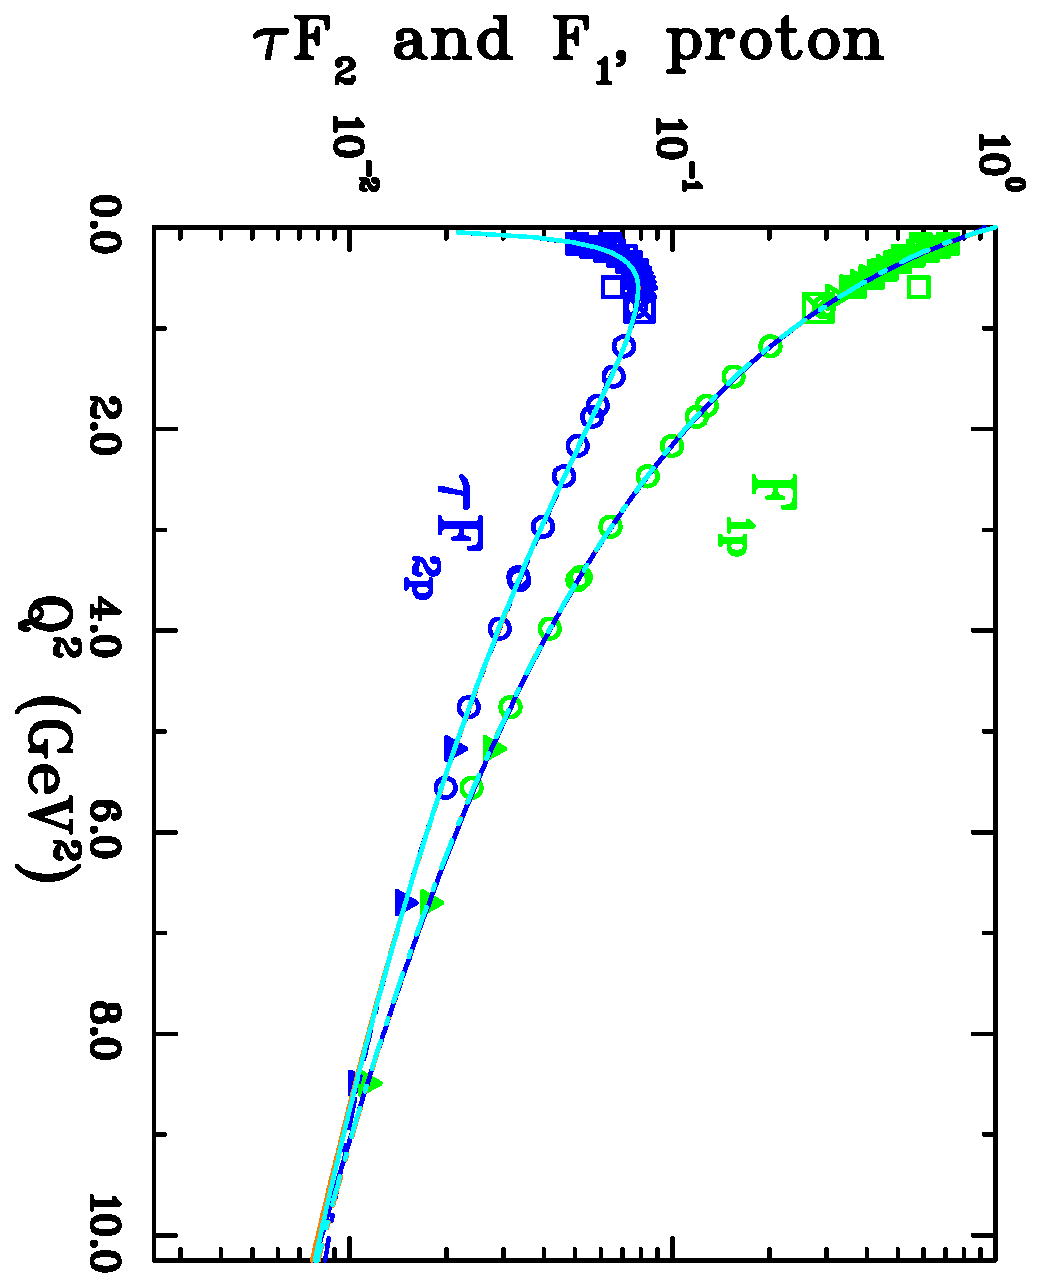
\includegraphics[angle=90]{f2andf1_11282014.eps}
}
\caption{The values of $F_1$ and $\tau F_2$  for the proton, obtained from the 3 JLab GEp experiments, and polynomial fits to them. From the definition of $G_E$, 
that form factor should cross zero when $F_1$ and $\tau F_2$ are equal. It can  be seen that this condition is satified near Q$^2$ = 10 GeV$^2$. See also Fig 
\ref{fig:f2andf1magn}.}
\label{fig:f2andf1}
\end{center}
\end{figure}

%%%%%%%%%%%%%%%%%%%%%%%%%%Figure 18
\begin{figure}
\begin{center}
\resizebox{0.45\textwidth}{!}{%
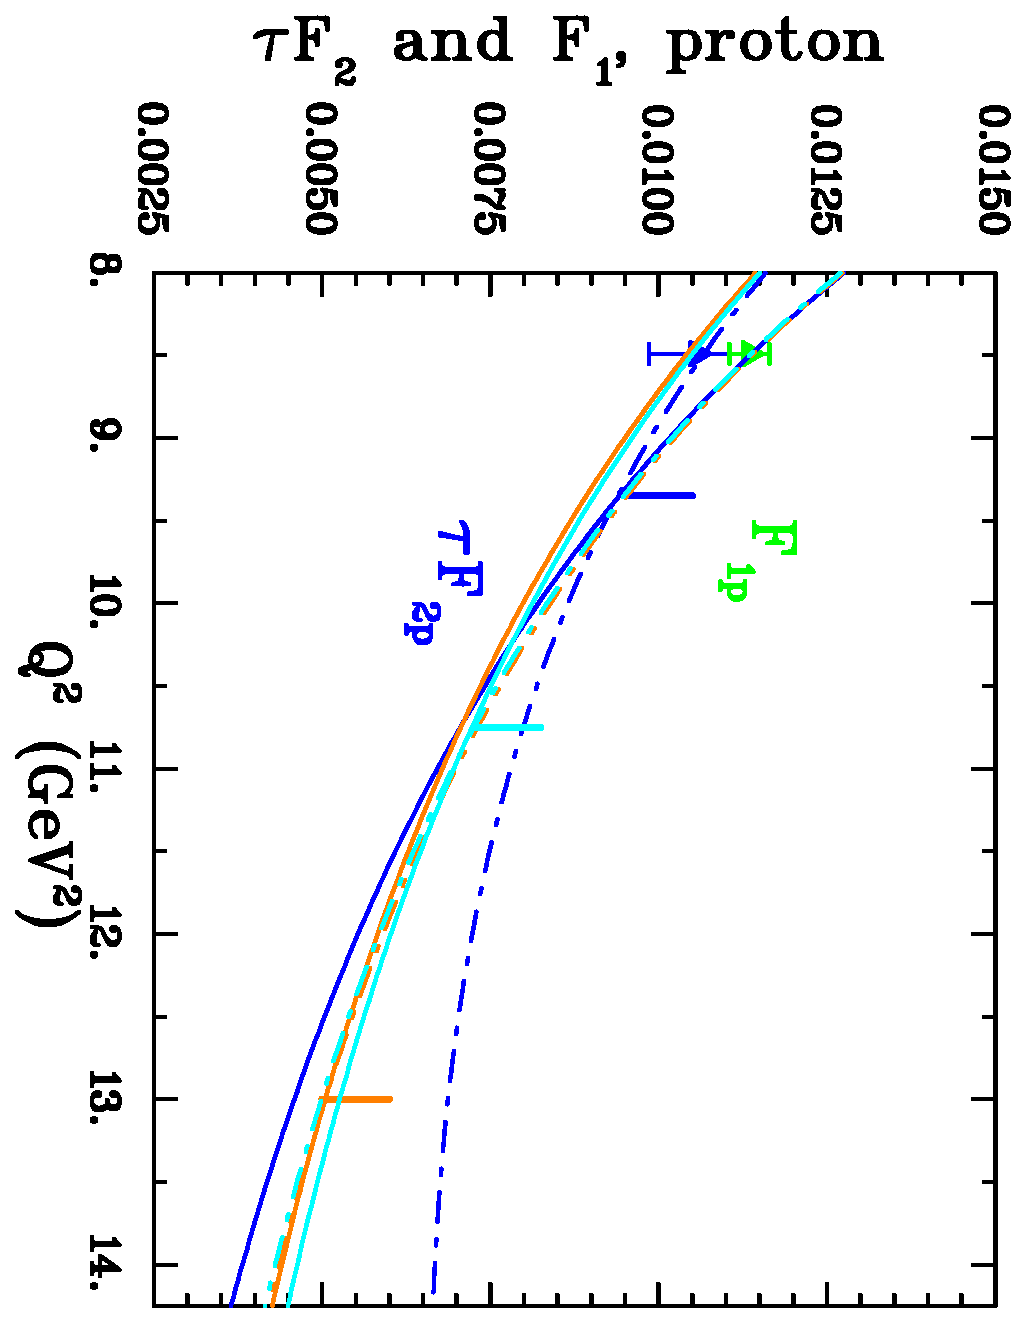
\includegraphics[angle=90]{f2andf1_magn_11282014.eps}
}
\caption{Magnification of the Q$^2$ = 12 GeV$^2$ region of Fig. \ref{fig:f2andf1}, showing 3 different positions for the zero crossing of $G_E$, marked as coloured 
vertical bars, for the 3 different fitting functions used: blue for an ad hoc polynomial of order 6 in Q, even and odd powers included; red ratio of polynomials with equal maximum power of Q$^2$, hence asymptotically constant; green, same as last but with $\frac{1}{Q^2}$ asymptotic behavior.}
\label{fig:f2andf1magn}
\end{center}
\end{figure}


%%%
%\end{document}






{\tiny }\section{Theoretical Interpretations of Nucleon Form Factors}
\label{sec:theory}

Placeholder text.

In this section we give an overview of the theoretical understanding 
of the nucleon e.m. FFs. 
These FFs encode the information on the structure of a  
strongly interacting many-body system of quarks and gluons, 
such as the nucleon. 
This field has a long history and many theoretical 
attempts have been made to understand the nucleon FFs. 
This reflects the fact that a direct calculation of nucleon FFs from the 
underlying theory, Quantum Chromodynamics (QCD), is complicated as it 
requires, in the few GeV momentum transfer region,  
non-perturbative methods. Hence, in practice it involves approximations 
which often have a limited range of applicability. 
Despite their approximations and limitations, some of these non-perturbative 
methods do reveal some insight in the nucleon structure. 
\newline
\indent
The earliest models to explain the global features of the nucleon FFs, such 
as its approximate dipole behavior, were vector meson dominance (VMD) models 
which are discussed in Sect.~\ref{theory_dispersion}. 
In this picture the photon couples to the nucleon through the exchange of 
vector mesons. Such VMD models are a special case of more general dispersion 
relation fits, 
which allow to relate time-like and space-like FFs, and which are
discussed subsequently. 
\newline
\indent
To understand the structure of the nucleon in terms of quark and gluon degrees
of freedom, constituent quark models have a long history. We discuss the 
intricacies in describing a bound system of relativistic constituent quarks 
and review the resulting predictions for FFs in Sect.~\ref{theory_models}. 
Despite some of their successes, models based on quarks alone do suffer from 
the evident shortcoming that they do not satisfy the global chiral symmetry 
of QCD when rotating left and right handed light quarks in flavor space. 
This chiral symmetry is broken spontaneously in nature, 
and the resulting Goldstone bosons are pions. Since they are the lightest 
hadrons, they dominate the low momentum transfer behavior of form factors, 
and manifest themselves in a pion cloud surrounding the nucleon. Such pion
cloud models will also be discussed in Sect.~\ref{theory_models}. 
\newline
\indent 
In Sect.~\ref{sec:rad}, we discuss the spatial 
information which can be obtained from the nucleon FFs, and discuss 
both radial densities and the issue of shape of the nucleon. 
\newline
\indent
Sect.~\ref{theory_eft} describes the chiral 
effective field theory of QCD and their predictions for nucleon FFs at low 
momentum transfers, where such perturbative expansions are applicable. 
\newline
\indent
In Sect.~\ref{sec:lattice}, we shall discuss the lattice QCD simulations, 
which have the potential to calculate nucleon FFs from first principles. 
This is a rapidly developing field and important progress has been made in the 
recent past. Nevertheless, the lattice calculations 
are at present still severely limited by available computing 
power and in practice are performed for quark masses sizably larger than their 
values in nature. We will discuss the issues in such calculations and compare 
recent results. It will also be discussed how the chiral effective field
theory can be useful in extrapolating present lattice QCD calculations to the 
physical pion mass.  
\newline
\indent
In Sect.~\ref{theory_gpd}, we discuss the quark structure of the nucleon and 
discuss generalized parton distributions (GPDs) of the nucleon. 
These GPDs are being accessed in hard exclusive reactions, which allow to 
remove in a controlled way a quark 
from the initial nucleon and implanting instead another quark in the final 
nucleon. The resulting GPDs can be interpreted as quark correlation functions 
and have the property that their first moments exactly coincide with the
nucleon FFs. We discuss the information which has been obtained on GPDs 
from fits of their first moments to the precise FF data set.   
\newline
\indent
Finally, in Sect.~\ref{theory_pqcd}, we discuss the nucleon FFs in the 
framework of perturbative QCD. These considerations are only valid 
at very small distances, where quarks nearly do not interact. In this limit, 
the nucleon FFs correspond to a hard photon which hits a valence quark 
in the nucleon, which then shares the momentum with the other (near collinear)
valence quarks through gluon exchange. 
We discuss the predictions made in this limit and confront them with the
experimental status for Dirac and Pauli FFs at large momentum transfers.


\subsection{Models of Nucleon Form Factors}
\label{subsec:models}

%
\subsubsection{Conformal fits to Form Factors}
\label{subsubsec:cf}

There has been a lively, at least to those engaged in it, discussion of what sorts of functions to use in fitting the form factors.  Simple polynomial fits, for example,  will not converge for moderate or large momentum transfers.   The reason flows from the fact that the form factors are, from a mathematical viewpoint, analytic functions of their argument $Q^2 = -q^2$, except for cuts at known locations.  The cuts are on the timelike side, and begin where one can have a photon to two pion transition at $q^2 = 4 m_\pi^2$.  A cut can be viewed as a weighted continuum of poles, so that there is a contribution to the form factor containing a factor $1/(q^2 - 4 m_\pi^2)$.  The weighting of this pole may be weak, but in principle its existence means that a polynomial expansion of the form factor will not converge for $Q^2 \ge 4 m_\pi^2$.  It is like the expansion of the geometric series $1/(1-x)$, which does not converge for $|x| \ge 1$;  simply replace $x$ by $q^2/(4m_\pi^2)$.

However, it is possible to make a mapping of $Q^2$ to another variable, denote it $z$, where a polynomial expansion in $z$ is allowed.  The trick is to find a transformation where spacelike momentum transfers all map onto the real line $|z| < 1$ and timelike momentum transfers map onto the circle $z =1$ (in the complex $z$-plane).  Then since all poles of the form factors lie on the unit circle in $z$, a polynomial expansion in $z$ is convergent everywhere inside the unit circle, \textit{i.e.,} for all spacelike momentum transfers.

This trick has been applied in the context of Weak interaction form factors, as for semileptonic meson decay, for some time~\cite{Boyd:1995sq,Bourrely:2008za}.  It has more recently been applied to fitting electromagnetic form factors~\cite{Hill:2010yb,Lorenz:2014vha}.

The variable $z$ can be given by the conformal mapping~\cite{Hill:2010yb,Lorenz:2014vha}, with $t = q^2$,
\begin{equation}
z(t,t_{\rm cut}) = \frac{ \sqrt{t_{\rm cut} - t} - \sqrt{t_{\rm cut}}}
					{ \sqrt{t_{\rm cut} - t} + \sqrt{t_{\rm cut}}}	\,,
\end{equation}
where $t_{\rm cut} = 4 m_\pi^2$ and one can easily enough verify that the mapping has the properties stated above.

Fitting with a nonconvergent expansion can give good analytic fits to the data in any region where there is data to be fit.  The danger lies in extending them outside the region where there is data.  Such extrapolations can go awry,  sometimes diverging wildly from physical expectation and sometimes, depending on how far one extrapolates, there may be problems that are less visible.  Here enters also the proton radius question, whose evaluation from form factors requires an extrapolation from the lowest $Q^2$ where there is data down to $Q^2 = 0$.  Extrapolating a fit made with an intrinsically convergent expansion is arguable safer.

The two fits made to the electromagnetic form factors using the conformal variable $z$, however, differ in their conclusions regarding the proton charge radius.  The earlier fit~\cite{Hill:2010yb}  used electron-proton scattering data available before the Mainz experiment~\cite{Bernauer:2010wm} published in 2010.   They found a proton radius $R_E^p =  0.870\pm 0.023 \pm 0.012$,  so their central value is closer to the CODATA value than to the muonic Lamb shift value.  The other fit~\cite{Lorenz:2014vha} used the 1422 data points from the Mainz experiment, and obtained $R_E^p = 0.840 \pm 0.015$ fm (see also~\cite{Lorenz:2014yda}).



%%%%%%%%

\subsubsection{Vector Meson Dominance (VMD)}
\label{subsubsec:vmd}

%%%%%%%%%%%

Placeholder text

The starting point in understanding the interaction of a vector probe 
such as the photon with a hadronic system is provided by the observation 
that the lowest lying hadrons with vector quantum numbers 
are the vector mesons $\rho(770)$, $\omega(782)$ and $\phi(1020)$. 
In the process $e^+ e^- \to hadrons$, these vector mesons show up as 
prominent resonances at the corresponding values of the $e^+ e^-$  
squared $c.m.$ energy $q^2 > 0$. 
One therefore expects that in the elastic electron scattering process 
on the nucleon, $e N \to e N$, the nucleon electromagnetic FFs 
at low space-like momentum transfers, $q^2 < 0$, will be dominated by these 
lowest lying singularities from the time-like region. 
A large class of models for $F_1$ and $F_2$ are based on this vector 
meson dominance (VMD) hypothesis, as depicted in~\ref{vmd}.
%
\begin{figure}[h]
\centerline{
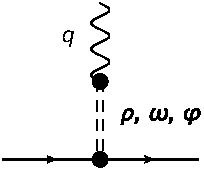
\includegraphics[width = 3 cm]{ff_vmd.pdf}
}
\caption{\small The vector meson dominance picture for the coupling of the  
photon (with four-momentum $q$) to a nucleon. }
\label{vmd}
\end{figure}
%
\newline
\indent
Within such VMD models, the approximate dipole behavior of the nucleon 
e.m. FFs, see Eq.~(\ref{eq:dipole}), can be understood as being due to the 
contribution of two nearby vector meson poles which have opposite residua. 
Assume that one considers two vector meson pole contributions in \ref{vmd} 
(with masses $m_{V1}$ and $m_{V2}$ 
and residua of equal magnitude and opposite sign $a$ and $-a$ respectively), 
one obtains~:
\begin{eqnarray}
F_{1,2} (q^2) &\sim& \frac{a}{q^2 - m_{V1}^2} + \frac{(-a)}{q^2 - m_{V2}^2} 
			\nonumber\\
&=& \frac{a \, (m_{V1}^2 - m_{V2}^2)}{(q^2 - m_{V1}^2) (q^2 - m_{V2}^2)}.
\end{eqnarray}
\indent
An early VMD fit was performed by Iachello {\it et al.}~\cite{iach} and  
predicted a linear decrease of the proton $G_{Ep} / G_{Mp}$ ratio, which 
is in basic agreement with the result from the polarization transfer 
experiments. Such VMD models have been extended by Gari and 
Kr\"umpelmann~\cite{gari} to include the perturbative QCD (pQCD) 
scaling relations~\cite{brodlep}, which 
state that (see Sect.~\ref{theory_pqcd}) $F_1 \sim 1/Q^4$, and  
$F_2 / F_1 \sim 1/Q^2$.
\newline
\indent
In more recent years, extended VMD fits which provide 
a relatively good parameterization of  
all nucleon e.m. FFs have been obtained. An example is Lomon's 
fit~\cite{lomon}, using $\rho(770)$, $\omega(782)$, $\phi(1020)$, 
and $\rho^\prime(1450)$ mesons and containing 11 parameters. 
Another such recent parameterization 
by Bijker and Iachello~\cite{bijker} including 
$\rho(770)$, $\omega(782)$, and $\phi(1020)$ mesons only achieves a 
good fit by adding a phenomenological contribution attributed to a 
quarklike intrinsic $qqq$ structure (of $rms$ radius $\sim 0.34$~fm) 
besides the vector-meson exchange terms. The pQCD scaling relations are 
built into this fit which has 6 free parameters which are fit to the data. 
In contrast to the early fit of Ref.~\cite{iach}, the new fit of 
Ref.~\cite{bijker} gives a very good description of the neutron data, 
albeit at the expense of a slightly worse fit for the proton data. 
\newline 
\indent
It will be interesting to check the resulting VMD fits 
for the neutron FFs to larger $Q^2$. 
In this regard, an interesting ``prediction'' can be drawn when the FFs 
$F_2$ and $F_1$ obtained directly from double
polarization experiments are shown in the same graph for the 
proton and the neutron, as in Fig.~\ref{fig:f2andf1}. 
It is remarkable that both $F_1$ and $F_2$ tend toward the 
same value for proton and neutron, and may meet at a $Q^2$ value 
which will soon be accessible for the neutron. 
This conclusion is influenced by the VMD fits shown in the same figure, 
and rests on their extrapolation for the neutron to larger $Q^2$.  
Note that the VMD fits shown include all data for p and n, 
but selects the recoil polarization over the Rosenbluth results 
for $Q^2$ larger than 1 GeV$^2$.  


%
\begin{figure}[h]
\begin{center}
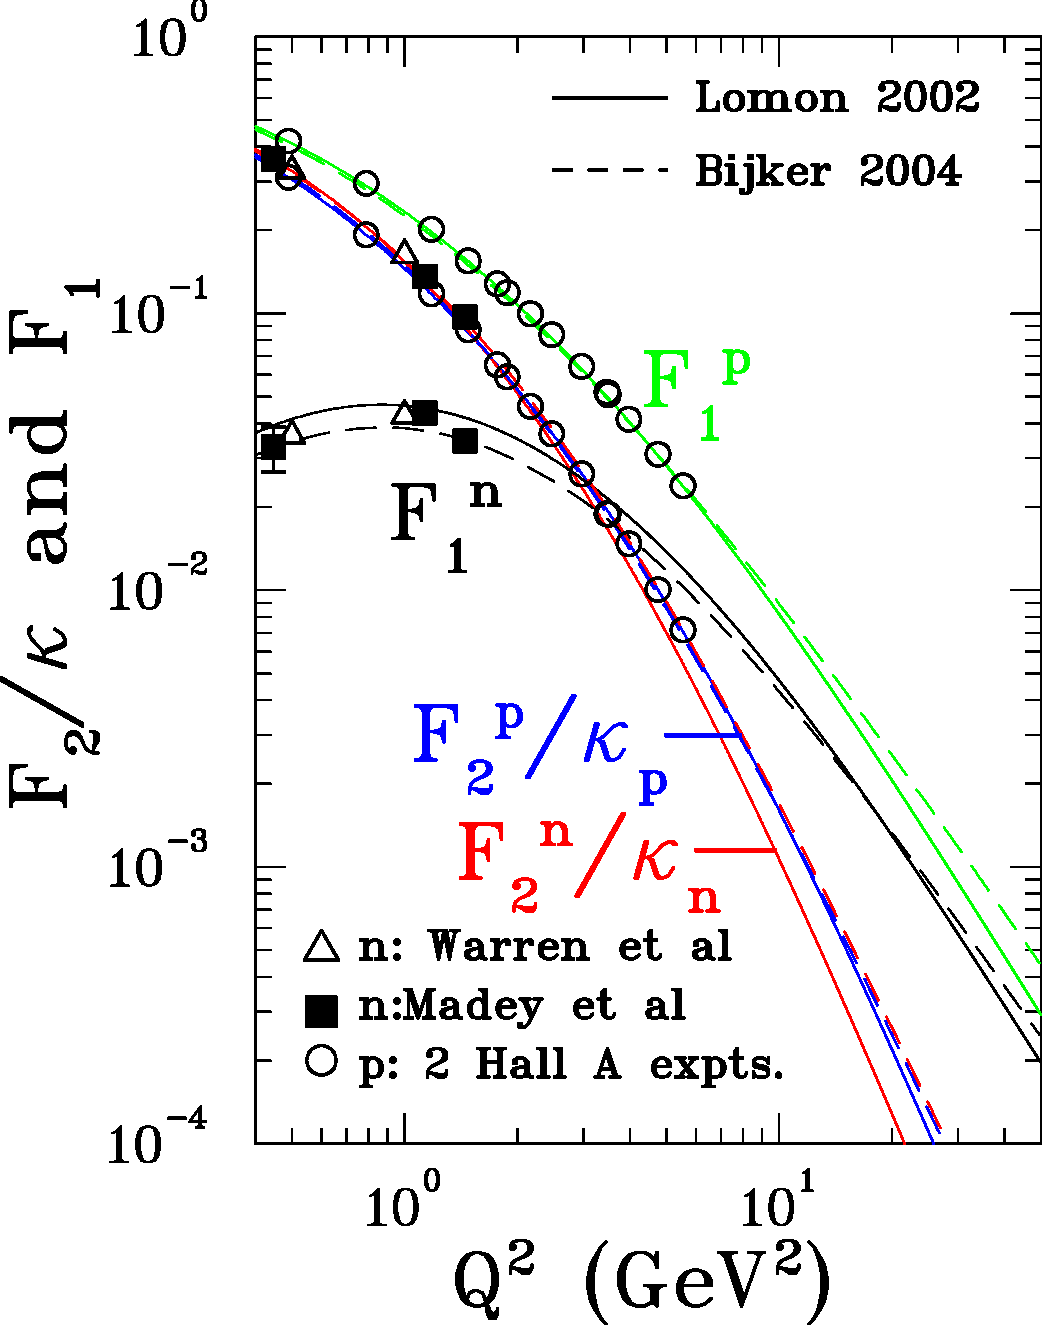
\includegraphics[width = 2.5 in]{f2andf1_pandn_col.pdf}
\caption{\small The FFs $F_1$ and $F_2$ for the proton and the neutron obtained
from double polarization experiments only.
The values of $F_2$ and $F_1$ were obtained from the experimental FF ratios
using fitted values to the data base for $G_{Mp}$ and $G_{Mn}$. 
For the proton data, the fit from \cite{kelly04} was used; 
for the neutron data in \cite{madey} the fit from \cite{kelly04}, and 
in \cite{warren} the fit from \cite{kubon} were used. 
The curves are the VMD fits of Lomon~\cite{lomon}
and of Bijker and Iachello~\cite{bijker}.}
\label{fig:f2andf1}
\end{center}
\end{figure}




\subsubsection{Dispersion Analyses}
\label{subsubsec:da}

Newer works here include the dispersive analyses of the nucleon form factors by workers in Bonn~\cite{Lorenz:2012tm,Lorenz:2014vha,Lorenz:2014yda}.  Older works include~\cite{Baldini:2005xx,Belushkin:2006qa,BaldiniFerroli:2012pr}.  The works include general analyses and fits to the form factors, as well as aspects directly aimed at the resolution of the proton radius puzzle~\cite{Lorenz:2012tm,Lorenz:2014vha,Lorenz:2014yda}.

Dispersion relations relate the form factors in the spacelike and timelike regions.  More generally, the form factors are complex functions of $q^2$ that are analytic except for known cuts, and the form factors anywhere can be calculated if one knows just their imaginary parts at the cuts.  The cuts are all on the real axis for timelike $q^2$.  The cuts run from $q^2 \approx 4 m_\pi^2$ to $q^2 = \infty$.  In practice, one cannot know the imaginary part of the form factors over this whole range, and uncertainty in knowing the form factors in the timelike region builds nonlinearly to larger uncertainty in predicting the form factors in the spacelike region, especially at higher $Q^2$.

At lower $Q^2$, one specific boon of the dispersive treatment is that the connection between the timelike and spacelike regions puts an extra constraint on the form factors and their slope at spacelike threshold.  This means that the determination of the charge and magnetic radii are not purely extrapolations of the scattering data, but is an interpolation in this procedure and hence arguably more reliable.

A technique for using the dispersion relations, used by both~\cite{Baldini:2005xx} and by~\cite{Lorenz:2012tm}, is to parameterize the imaginary part of the timelike form factors, and determine the parameters by making a least squares fit to the known spacelike and timelike data.  One thereby obtains a representation of the form factors that one can use in regions where there is not yet data.

Ref.~\cite{Baldini:2005xx}, published in 2006, applies dispersion relations to the ratio $G_E^p/G_M^p$, with the assumption of no zeros in $G_M^p$.  They used some large-uncertainty-limit $G_E^p/G_M^p$ data in the timelike region, obtained from angular distributions in $e^+ e^- \to p \bar p$ or the reverse, to supplement the polarization data in the spacelike region.  One of the main goals was to compare to models that fit the spacelike data, especially to the continuations of those models to the timelike regions~\cite{Brodsky:2003gs}.  

They found that there was a zero in $G_E^p(q^2)$ at about $11$ GeV$^2$ spacelike momentum transfer squared, and found that the Phragm\'en-Lindel\"of theorem, which leads to the statement that $|G_E^p(q^2)/G_M^p(q^2)|$ should be the same at very large momentum transfers, whether spacelike or timelike, was satisfied, albeit with opposite signs.  Many of the more purely phenomenological models differed on the latter point.  This work~\cite{Baldini:2005xx} preceded the completion of the polarization experiments at the highest current $Q^2$~\cite{puckett:2010,puckett:2011}.  The dispersive aspects have not been updated in more recent works by some of the same authors, \textit{e.g.}~\cite{BaldiniFerroli:2012pr}, but one can see that the results would not be materially changed by the newer data.

Ref~\cite{Lorenz:2012tm}, which is an updated version of~\cite{Belushkin:2006qa}, applies the dispersion analysis to $G_E^p$ and $G_M^p$ separately.  An important improvement in the newer work~\cite{Lorenz:2012tm} is that it includes the recent Mainz data~\cite{Bernauer:2010wm} in its fit.  A salient outcome of this analysis is that the proton charge radius comes out at a value $R_E^p = 0.84\, (1)$ fm, in agreement with the value found in the muon hydrogen Lamb shift measurement.

%%%%%%%%%%%
\subsubsection{Constituent Quark Models}
\label{subsubsec:cqm}

%%%%%%%%%%%

Placeholder text  

In our quest to understand the structure of the nucleon in 
terms of the quark and gluon degrees of freedom which appear in the 
QCD Lagrangian, 
constituent quark models (CQMs) have a long history, which predates the 
establishment of the theory of strong interactions, QCD.
In a CQM, the nucleon appears as the ground state 
of a quantum-mechanical three-quark system in a confining potential.
In such a picture, the ground state baryons (composed of the 
light up ($u$), down ($d$) and strange ($s$) quark flavors) are 
described by $SU(6)$ spin-flavor wave functions (WFs), supplemented 
by an antisymmetric color WF.  
\newline
\indent
In the Isgur-Karl model~\cite{isgur}, 
the constituent quarks  
move in a harmonic oscillator type confining potential. 
For the ground state baryons, 
the three constituent quarks are in the $1s$ 
oscillator ground state, corresponding to the [56]-plet of $SU(6)$. 
In the Isgur-Karl model, the long-range confining potential is supplemented by 
an interquark force corresponding to one-gluon exchange. 
The one-gluon exchange leads to a color hyperfine interaction 
between quarks, which 
breaks the $SU(6)$ symmetry and leads to a mass splitting 
between $N(939)$ and $\Delta(1232)$, often referred to as the hyperfine 
splitting. 
It was found that it also predicts well the mass splittings between octet 
and decuplet baryons~\cite{derujula}. 
Furthermore, the color hyperfine interaction leads to a tensor force  
which produces a small $D$-state ($L = 2$) admixture in the 
$N$ (as well as $\Delta$) ground states~\cite{Koniuk:1979vy,Isgur:1981yz},  
corresponding to a $D$-state probability in the $N$ ground state 
around 0.2~\%.    
Even though such $D$-wave probability is small, 
it leads to a non-spherical charge distribution.  
For a static charge distribution, a measure of  
the non-sphericity (or deformation) is given by its quadrupole moment.    
Since the nucleon has spin 1/2, 
an intrinsic quad\-rupole moment of the nucleon 
cannot be directly measured because angular momentum conservation 
forbids a non-zero matrix element of a ($L = 2$) quadrupole operator 
between spin 1/2 states. 
However this quadrupole deformation may reveal itself in an 
electromagnetically induced transition 
from the spin 1/2 $N$ to the spin 3/2 $\Delta$ state. 
In this way, the tensor force between quarks gives rise to non-zero values 
for the electric quadrupole ($E2$) and Coulomb quadrupole ($C2$) 
transitions\footnote{  
The relation between the tensor force, $D$-wave admixture,
and the electromagnetic $N \to \Delta$ transition 
was already pointed out in the early paper of 
Glashow~\cite{Glashow79}. An up-to-date discussion of this field 
can be found in the review of~\cite{PVY06}.}. 
\newline
\indent
The non-relativistic CQM, despite its simplicity, 
is quite successful in predicting the spectrum of 
low-lying baryons, and gives a relatively good 
description of static properties such as the octet baryon magnetic moments.  
To calculate the FFs of a system of constituents with  
masses small compared with the confinement mass scale necessitates however 
a relativistic treatment even for low momentum transfers. For momentum 
transfers several times the nucleon mass squared a relativistic description  
becomes crucial. 
\newline
\indent
In contrast to the calculation of the spectrum, which uses eigenfunctions 
of a Poincar\'e invariant mass operator, 
a calculation of the nucleon electromagnetic FFs requires 
the relation between the rest frame spin and momenta 
(in the three-quark WF) and those in the moving frame.  
This requires 
an extension of eigenfunctions of the spin and mass operators, 
so as to transform consistently under 
the unitary representations of the Poincar\'e group.  
The way to implement relativity into a Hamiltonian formalism 
(describing e.g. a system of three interacting constituent quarks) 
has been laid 
out by Dirac~\cite{dirac}. There are three {\it forms of dynamics} 
(so called instant, point, and light-front forms) which 
differ in the choice of the kinematical subgroup of the Poincar\'e group. 
This is the subgroup of the Poincar\'e group whose commutator relations 
are not affected by the interactions between the constituents. 
The three (unitarily equivalent) forms therefore 
differ by which of the ten generators of the Poincar\'e group 
(four space-time translations, three spatial rotations, and three boosts) 
are kinematical (i.e. interaction free),  
and which are dynamical, i.e. depend on the interactions and 
necessarily have to be approximated in a practical calculation. 
\newline
\indent
In the {\it instant form}, the dynamical generators are the time component 
of the four-momentum and the three boost operators.  
Rotations do not contain interactions, which makes it 
easy to construct states of definite angular momentum in this form. 
\newline
\indent
In the {\it point form}, both boosts and rotations are kinematical. 
The point-form therefore has the important 
technical advantage that the angular momenta and Lorentz boosts are the same 
as in the free case. However all four components of the four-vector operator 
are dynamical in this form.  
\newline
\indent
In the {\it light-front form}, seven of the generators of the Poincar\'e 
group are kinematical (this corresponds to the symmetry group of a 
null plane), which is the maximum number possible. The 
remaining three dynamical generators which contain the interactions 
are one component of the four-momentum operator (the so-called light-cone 
Hamiltonian) and 2 transverse 
rotations. Light-front (as well as point form) calculations 
for relativistic CQMs are convenient as they allow to boost 
quark WFs independently 
of the details of the interaction. The drawback of the light-front 
calculations however is that because two generators 
of rotations are dynamical, the construction of states with good 
total angular momentum becomes interaction dependent. 
\newline 
 \indent
Any practical calculation in one of the three forms approximates the 
current operator. The common (so-called impulse) approximation 
is that the photon 
interacts with a single quark in the nucleon. 
\newline
\indent
The light-front form calculation of nucleon FFs has been pioneered by 
Berestetsky and Terentev~\cite{Berestetsky}, and more recently developed  
by Chung and Coester~\cite{chung}. In practice one starts from a 
rest frame nucleon WF for the three-quark state which ideally 
is fitted to the baryon spectrum. The nucleon WF 
in the light-front form (so-called light-front WF) is obtained by 
a Melosh rotation ~\cite{Melosh:1974cu} 
of each of the quark spinors, connecting the instant and light-front forms.  
When performing the front form calculation in a (Drell-Yan) 
frame where the photon light-cone 
momentum~\footnote{Defining light-cone components as 
$x^\pm = (x^0 \pm x^3)/\sqrt{2}$ and defining the null-plane by $x^+ = 0$.} 
component $q^+ = 0$, the space-like virtual photon 
only connects Fock components in the nucleon light-front WFs with 
the same number of constituents, i.e. matrix elements between $qqq$ and 
$qqqq \bar q$ states which would be present in an instant form calculation 
are zero in the light-front calculation. 
This property allows for a consistent calculation within 
the light-front formalism when truncating the Fock space to only the 
three-quark state. 
\newline
\indent
In~\cite{chung} a Gaussian WF in the quark internal 
(transverse) momentum variables was used. Although this model yields a 
surprisingly good agreement for the observed $G_{Ep}/G_{Mp}$ ratio, 
see \ref{relcqm}, it yields nucleon FFs which 
drop too fast at larger $Q^2$ values when using constituent quark masses 
around 330 MeV.  
Schlumpf~\cite{schlumpf} allowed for high momentum components in the 
nucleon light-front WF by adopting 
a power law dependence in the 
quadratic quark internal momentum variables. The two parameters in Schlumpf's  
WF were fitted to magnetic moments and semi-leptonic decays of the 
baryon octet. The resulting e.m. FF calculations reproduce reasonably well 
the power behavior of the FF at larger $Q^2$. 
The WF of Schlumpf was also used 
by Frank, Jennings, and Miller~\cite{gamiller,miller02}. 
They found that such a light-front WF leads to a violation of 
hadron helicity conservation resulting in a  
$F_{2p}/F_{1p}$ ratio which drops less fast than 
$1/Q^2$~\cite{miller02}, in agreement with the $G_{Ep}/G_{Mp}$ polarization 
data.    

%%%%%%%%%%
\begin{figure}[h]
\begin{center}
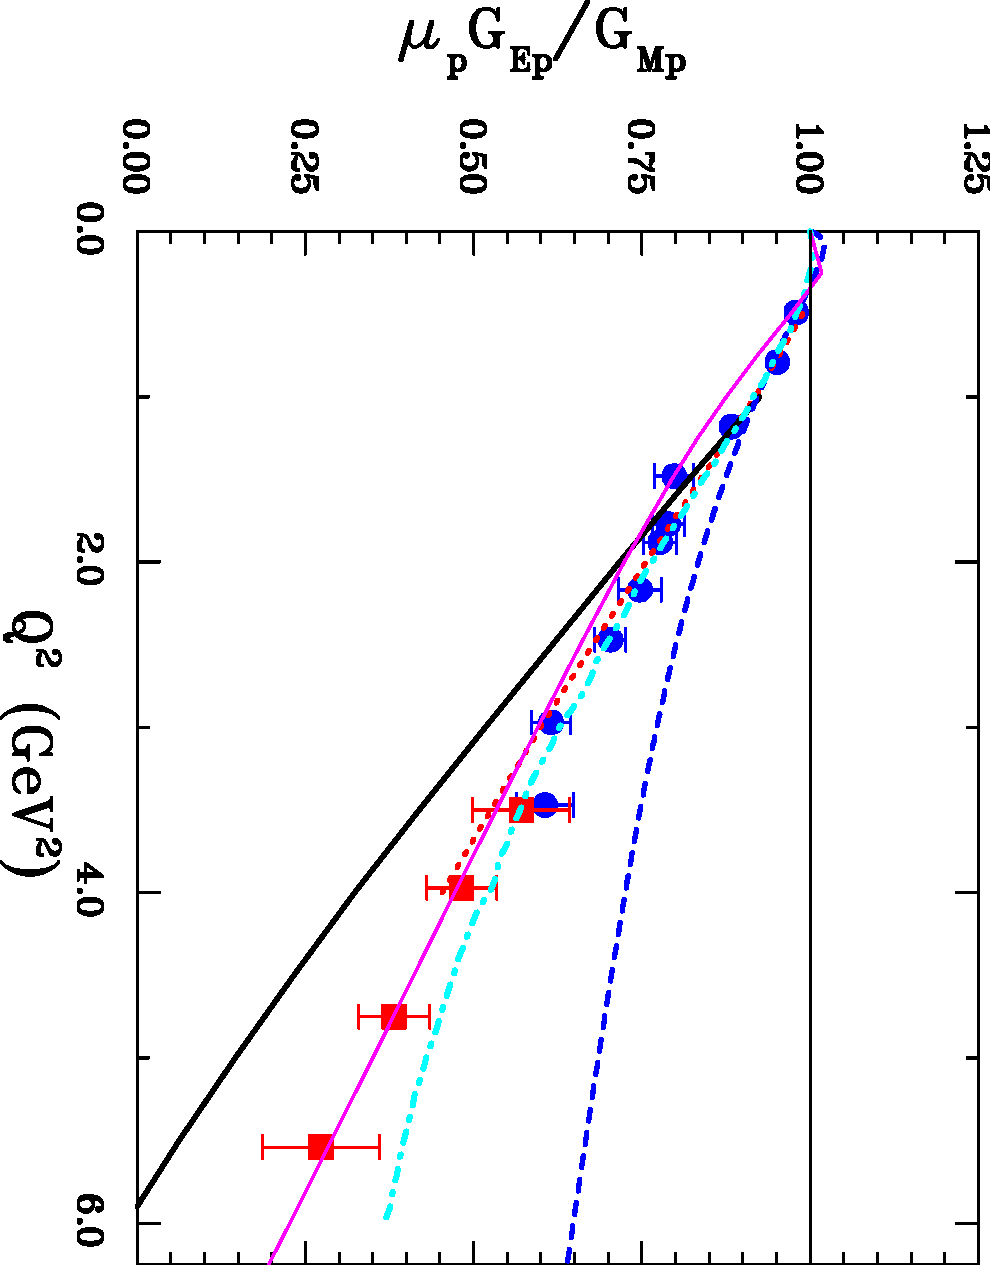
\includegraphics[width =5cm,angle=90]{gepgmp_jlab_vsCQM_col.pdf}
\end{center}
\vspace{-0.25cm}
\caption{\small Comparison of relativistic CQM calculations 
with the data for $\mu_p G_{Ep} / G_{Mp}$. 
Dotted curve : front form calculation of Chung and Coester~\cite{chung} 
with point-like constituent quarks; 
thick solid curve : front form calculation of Frank {\it et al.}~\cite{gamiller}; 
dot-dashed curve : front form calculation of 
Cardarelli {\it et al.}~\cite{rome,cardarelli} with point-like constituent quarks; 
dashed curve : point form calculation of Boffi et 
al.~\cite{boffi} in the Goldstone boson exchange model with point-like 
constituent quarks; 
thin solid curve : covariant spectator model of 
Gross and Agbakpe~\cite{gross}. 
The data are from~\cite{punjabi05} (solid circles) and  
\cite{gayou2} (empty squares). 
}
\label{relcqm}
\end{figure}

%%%%%%%%%%%

The WFs in the calculations described above were however not 
constructed from a detailed fit to the baryon spectrum. 
Cardarelli {\it et al.}  
subsequently performed a more ``microscopic'' light-front 
calculation~\cite{rome,cardarelli} 
where the light-front WF was obtained from a rest frame WF 
which provided a fit to the spectrum. 
The rest frame WF was taken from 
the relativized Capstick-Isgur model~\cite{Capstick:1986bm}.  
Using this WF, 
the constituent quark momentum distribution in the nucleon 
was found to yield an important content 
of high-momentum components, which are generated by the short-range 
part of the quark-quark interaction, which is due to one-gluon exchange in 
the Capstick-Isgur model. These components are completely absent if one only 
considers the linear confinement potential in the model. 
\newline
\indent
In a CQM calculation,  
the effect of other degrees of freedom beyond three quarks are 
buried within the constituent quarks, which are considered as quasi-particles. 
In the absence of a microscopic calculation, 
such effects are parameterized in terms of constituent quark FFs. 
In~\cite{Petronzio:2003bw}, 
it was shown that the data for the proton unpolarized forward 
structure function at low momentum transfers exhibits a new scaling 
property and can be interpreted as quasi-elastic scattering off extended 
constituent quarks inside the proton described by a 
constituent quark FF. The resulting constituent size is 
around 0.2 - 0.3 fm. 
Using such effective constituent quark FF in 
the light-front form calculation of~\cite{cardarelli}, 
allows a good description of the individual nucleon FFs, see~\cite{pace}.
Note however that the experimental $G_{Ep} / G_{Mp}$ ratio 
can basically be reproduced using point-like constituent quarks, 
see \ref{relcqm}. 
The suppression of the $G_{Ep}/G_{Mp}$ 
ratio with respect to the dipole-fit as predicted 
in the light-front form CQM calculation is 
attributed to relativistic effects generated by the Melosh rotations of the 
constituent quark spins. These Melosh rotations introduce kinematical 
$SU(6)$ breaking effects in addition to the dynamical 
$SU(6)$ breaking due to the (hyperfine) one-gluon exchange potential. 
\newline
\indent
A comparable amount of high-momentum components in the nucleon 
WF was obtained in the 
Goldstone-boson-exchange (GBE) 
quark model~\cite{Glozman:1997fs,Glozman:1997ag}.  
This model relies on constituent quarks and Goldstone 
bosons, which arise as effective degrees of freedom of low-energy QCD 
from the spontaneous breaking of the chiral symmetry. 
The resulting CQM assumes a linear confinement potential supplemented by 
a quark-quark interaction based on the exchange of pseudoscalar 
Goldstone bosons, which is the source of the hyperfine interaction. 
It was shown in~\cite{Glozman:1997fs,Glozman:1997ag}  that the GBE 
CQM yields a unified description of light- and strange-baryon spectra. 
The GBE CQM was used in~\cite{wagenbrunn,boffi} 
to calculate the nucleon e.m. FFs in the point-form. The neutron 
charge radius is well described in this model and is driven 
by the mixed-symmetry component in the neutron WF.  
In contrast to the light-front 
calculation~\cite{cardarelli,pace}, it was found that when performing 
a point-form calculation of the nucleon e.m. FFs at larger $Q^2$ 
within the impulse approximation, 
i.e. considering only single-quark currents, a surprisingly 
good overall description of the nucleon e.m. FFs can be obtained, using  
point-like constituent quarks only. 
When looking at details of Refs.~\cite{wagenbrunn,boffi}, 
the agreement is worse though for $G_{Mp}$ which 
is underpredicted at larger $Q^2$, and the ratio of $G_{Ep}/G_{Mp}$ is 
overpredicted at larger $Q^2$, see \ref{relcqm}. 
Similar findings have also been obtained in the point-form calculation 
of~\cite{Wagenbrunn:2005wk} for the OGE CQM. 
The overall success of the point-form result using point-like constituent 
quarks was attributed in~\cite{wagenbrunn,boffi,Wagenbrunn:2005wk} 
to the major role played by relativity.  
Such a finding is remarkable in view of the expected finite 
size of the constituent quarks, as discussed above.  
\newline
\indent
An explanation for the above finding for the nucleon 
e.m. FFs in the point form, 
using the single-quark current approximation, 
has been suggested by Coester and Riska~\cite{Coester:2003rw}. 
When the spatial extent of the three-quark WF 
is scaled (unitarily) to zero, both  
instant- and front-forms yield FFs independent of the momentum 
transfer. Therefore, to reproduce 
the experimental fall-off of the nucleon e.m. FFs  
at large momentum transfers requires the introduction of constituent quark 
FFs. In contrast, when the WF in point form is scaled unitarily to 
zero (so-called point limit), a non-trivial scaling limit is obtained for 
the FFs, depending on the shape of the WF. 
At high values of momentum transfer, the scaled FFs decrease with an inverse 
power of the momentum transfer. The power is determined 
by the current operator and is independent of the WF. 
An explicit comparative calculation of the baryon e.m. FFs 
between the three different forms was performed in~\cite{Julia-Diaz:2003gq} 
using a simple algebraic form 
for the three-quark WF, depending on two parameters. 
It was verified that a qualitative description of the nucleon FF data 
demands a spatially extended WF in the 
instant- and front-form descriptions, in contrast to 
the point-form description which demands a much more compact WF.  
\newline
\indent
A manifestly covariant CQM calculation within the Bethe-Salpeter formalism 
and using an instanton-induced interaction between quarks has been performed 
by Merten {\it et al.}~\cite{Merten:2002nz}. Although this model 
reproduces the baryon spectrum, it can only qualitatively 
account for the $Q^2$ dependence of the nucleon e.m. FFs. 
\newline
\indent
Another covariant CQM calculation was performed by 
Gross and Agbakpe~\cite{gross}, using a covariant spectator model. 
Assuming a simple pure $S$-wave form for the nucleon three-quark wave 
function, evaluating the current matrix element in 
a relativistic impulse approximation, and assuming constituent quark FFs 
including a phenomenological term which parameterizes the pion cloud, 
an eleven parameter description of the nucleon FF data was obtained, 
see \ref{relcqm}. 
\newline
\indent
As a next step for CQMs, it would clearly be very worthwhile to investigate 
the approximations in the current operator within each form.
The quality of the commonly made impulse approximation 
may differ between the different forms. 
Within the context of a toy model calculation in 
Refs.~\cite{Desplanques:2003nk,Desplanques:2005vu}, 
it has e.g. been shown that the neglect of two-body currents in the point form 
does affect the FFs in a more drastic way than their neglect in the instant 
or light-front forms. 
\newline
\indent
The importance of two-body currents has also been 
shown in the work of De Sanctis {\it et al.}~\cite{Desanctis}. 
In that work, a calculation 
within the hypercentral CQM was performed of the (two-body) quark pair 
contribution to the e.m. current resulting from the 
one-gluon exchange interaction between the quarks. This pair current 
contribution was found to lead to a sizeable reduction of $G_{Ep}$ 
compared with $G_{Mp}$.  



%%%%%%%%%%%%%%%%%%%%
\subsubsection{Pion Cloud Models}
\label{subsubsec:pion}

%%%%%%%%%%%%%%%%%%%%%%%%%%%%%%%%%%%%%

Placeholder text

Despite their relative success in describing the spectrum and structure of 
low-lying baryons, models based on constituent quarks alone 
suffer from evident shortcomings as they do not satisfy all symmetry 
properties of the QCD Lagrangian. In nature, the up and down (current) quarks 
are nearly massless. In the exact massless limit, the QCD Lagrangian is 
invariant under $SU(2)_L \times SU(2)_R$ rotations of left ($L$) and 
right ($R$) handed quarks in flavor space. This {\it chiral symmetry} 
is spontaneously broken in nature leading to the appearance of massless 
Goldstone modes. For two flavors, there are three Goldstone bosons ---
pions, which acquire a mass due to the explicit breaking of chiral 
symmetry by the current quark masses. 
\newline
\indent
Since pions are the lightest hadrons, they 
dominate the long-distance 
behavior of hadron WFs and yield characteristic 
signatures in the low-momentum transfer behavior of hadronic 
FFs. 
Therefore, a natural way to qualitatively improve 
on the above-mentioned CQMs is to include the pionic degrees of freedom 
~\cite{Manohar:1983md}.  
\newline
\indent
An early quark model with chiral symmetry 
is the chiral (or, cloudy) bag model. This model  
improves the early MIT bag model by introducing 
an elementary, perturbative pion which couples to quarks in the bag 
in such a way that chiral symmetry is restored~\cite{Thomas:1982kv}. 
Within the cloudy bag model, Lu {\it et al.}~\cite{lu} 
performed a calculation of the nucleon e.m. FFs 
improving upon previous calculations by 
applying a correction for the center-of-mass motion of the bag. 
This calculation also implemented Lorentz covariance in an approximate way 
by using a prescription for the Lorentz contraction of the 
internal structure of the nucleon. Using a bag radius $R \simeq 1$~fm, 
this model provides a good description of the nucleon e.m. FFs in the range 
$Q^2 < 1$~GeV$^2$.  
\newline
\indent
To extend such a calculation to larger $Q^2$, Miller performed a 
light-front cloudy bag model calculation~\cite{miller02b}. 
Starting from a model in terms of constituent quarks~\cite{miller02}, 
described by the light-front WF of Schlumpf, 
the effects of the pion cloud were 
calculated through one-loop diagrams, including relativistic 
$\pi N N$ vertex FFs. The model gives a relatively good gobal 
account of the data both at low $Q^2$ and larger $Q^2$, 
though tends to show too much structure around the dipole form 
for the magnetic FFs at low $Q^2$. 
\newline
\indent
The cloudy bag model is one chiral quark model which 
treats the effect of pions perturbatively. Other quark models 
which calculated nucleon e.m. FFs using perturbative pions can be found 
e.g. in the early works of~\cite{Oset:1984tv,Jena:1992qx}, as well as in 
the already discussed works of~\cite{Glozman:1997fs,Glozman:1997ag}.  
Recently, the above chiral quark models where pions are included 
perturbatively have been improved in~\cite{faessler}. 
This work extends a previous work of ~\cite{Lyubovitskij:2001nm} by 
dynamically dressing bare constituent quarks by mesons to fourth order 
within a manifestly Lorentz covariant formalism. 
Once the nucleon and $\Lambda$ hyperon magnetic moments are fitted, 
other e.m. properties, such as the
nucleon e.m. FFs at low momentum transfers, follow as a prediction. 
It was found in~\cite{faessler} 
that the meson cloud is able to nicely describe 
the FF data in the momentum transfer region up to about 0.5 GeV$^2$.  
To extend the calculations to larger $Q^2$, a phenomenological approach 
has been adopted in \cite{faessler} by introducing 
bare constituent quark FFs which were parameterized 
in terms of 10 parameters. Such parameterization makes it plausible to 
simultaneously explain the underlying dipole structure in the nucleon e.m. FF
as well as the meson cloud contribution at low $Q^2$ which results from 
the underlying chiral dynamics. In a later paper~\cite{Faessler:2006ky}, a 
model calculation for the bare constituent quark FFs has been performed and 
applied to the e.m. properties of the $N \to \Delta$ transition. 
\newline
\indent
When pion effects dominate nucleon structure, their effects have to be 
treated non-perturbatively. A non-perturbative 
approach which has both quark and pion degrees of freedom 
and interpolates between a CQM and 
the Skyrme model (where the nucleon appears as a soliton solution of an 
effective nonlinear pion field theory) is 
the chiral quark soliton model ($\chi$QSM). 
As for the Skyrme model, 
the $\chi$QSM is based on a $1/N_c$ expansion  
(with $N_c$ the number of colors in QCD).  
Its effective chiral action has been
derived from the instanton model of the QCD vacuum \cite{Dia86}, which
provides a natural mechanism of chiral symmetry breaking 
and enables one to generate dynamically the constituent 
quark mass.  
Although in reality the number of colors $N_c$ is equal to three, 
the extreme limit of large $N_c$ is 
known to yield useful insights. At
large $N_c$ the nucleon is heavy and can 
be viewed as $N_c$ ``valence" quarks bound by a self-consistent pion
field (the ``soliton")~\cite{Dia88}.
A successful description of static properties of baryons, 
such as mass splittings, axial constants, magnetic moments, 
FFs, has been achieved (typically at the 30 \% level or better, 
see~\cite{Chr96} for a review of early results). 
After reproducing masses and decay constants in the mesonic sector, 
the only free parameter left to be fixed in the baryonic sector
is the constituent quark mass. 
When taking rotational ($1/N_c$) corrections into account, 
this model achieved a qualitative good description of the nucleon e.m. 
FFs in the range $Q^2 < 1$~GeV$^2$, using a constituent 
quark mass around $420$~MeV~\cite{Christov:1995hr}.
The chiral soliton model naturally accounts for the decrease of the 
$G_{Ep} / G_{Mp}$ ratio with increasing $Q^2$. This can be understood 
from the hedgehog structure in soliton models which couples spatial rotations 
with isorotations. In the soliton rest frame, the isovector electric FF 
$G_E^V$ therefore measures the rotational inertia density $\rho^V(r)$, in 
contrast to the isoscalar electric FF $G_E^S$ which measures the 
isoscalar baryon density $\rho^S(r)$. For a rigid rotor, 
the inertia density is obtained from the baryon density as 
$\rho^V = r^2/r_B^2 \, \rho^S$, with $r_B$ a free parameter characterizing 
the spatial extent. Assuming a Gaussian density for $\rho^S(r)$, 
this yields~\cite{holzwarth}~:
\begin{eqnarray}
\frac{\mu_p G_{Ep}(Q^2)}{G_{Mp}(Q^2)} = 
1 - \frac{1}{18} Q^2 r_B^2. 
\label{eq:gegmsol}
\end{eqnarray} 
With the choice $r_B^2 \approx (0.3 \, \mathrm{fm})^2$, one can obtain an 
excellent fit of the polarization data for $G_{Ep}/G_{Mp}$. 
Although in the chiral soliton model calculation 
the baryon density is not exactly Gaussian, 
and the rigid rotor calculation does not hold exactly, these relations can be 
considered as approximate relations~\cite{holzwarth}. 
\newline
\indent
Holzwarth~\cite{holzwarth} extended the chiral soliton model by including the 
$\rho$ ($\omega$) meson propagators for the isovector (isoscalar) channels 
respectively. Furthermore, to extend the range in $Q^2$ of the predictions, 
he uses a relativistic prescription to boost the soliton rest frame densities 
to the Breit frame. Such prescription is also used to extract 
radial charge and magnetization rest frame densities 
from experimental FFs, as will be discussed in Sect.~\ref{sec:rad}. 
Using 4 fit parameters (one effective boost mass and three free parameters 
to fix the couplings of $\rho$ and $\omega$ mesons), 
the model was found to provide a good account of 
the detailed structure of the nucleon e.m. FFs in the low $Q^2$ region. 
In particular, for $G_{Ep}/G_{Mp}$ it 
predicts a decreasing ratio in good agreement with the data. 
At larger $Q^2$, the boost prescription gives a reasonably good account of the 
data (except for $G_{Mn}$) and predicts a zero in $G_{Ep}$ around 
10~GeV$^2$. Due to the uncertainty introduced from 
the particular choice for the boost prescription, the 
high $Q^2$ behavior (for $Q^2$ larger than about $4 M^2$) 
of the e.m. FFs is however not a profound prediction of the 
low-energy effective model.  

%%%%%%%%%%%%%%%%

\subsection{Dyson-Schwinger Equations and Diquark Models}
\label{subsec:dse}

%%%%%%%%%%%%%%%%%

The Dyson Schwinger equations (DSE) are generically a non-perturbative approximation for obtaining results for a field theory, in the present case QCD.  The equations are, in principle, an infinite set of coupled integral equations.  In practice, they must be truncated, in a way that preserves all symmetries of QCD, in order to proceed with any calculation. For a general DSE review, see~\cite{Bashir:2012fs}.   

One accomplishment of the DSE follows the solution for the full quark propagator, represented in momentum space as
\begin{equation}
S_F(p^2) = \frac{ i F(p^2) }{ \not\! p + M(p^2) }	\,,
\end{equation}
where the normalization $F(p^2)$ and the mass $M(p^2)$ become functions of momentum because of interactions.  With relatively simple truncations and modeling of the QCD interactions, the DSE obtain a mass function in good agreement with lattice calculations.  The mass $M(p^2)$ is several hundred MeV at small $p^2$ and falls smoothly to the small values at large $p^2$ that one might expect in perturbation theory.

Also early in the DSE program is building a model of the quark-quark and quark-antiquark interactions that will reproduce data on, among other quantities, the pion mass and decay constant.

One then uses the same quark-quark interactions developed in meson studies to obtain a three quark wave function model for the nucleon by solving the three-cody Fadeev equations.  There arise significant diquark, \textit{i.e.,} significant quark-quark correlations, that have a strong effect on the form factors one obtains.  Since the quarks in this model are dressed,  many of their features are different from expectations for pointlike fermions.  One finds in particular large quark anomalous chromomagnetic moments, which affect the quark-gluon interactions, which lead to large quark anomalous magnetics moments in the quark-photon interactions, which in turn are needed to obtain good fits to the nucleon electromagnetic form factor data.  

The theoretical DSE results~\cite{Cloet:2014rja,Cloet:2013gva,Cloet:2013jya} show a falloff of the $G_E^p$/$G_M^p$ ratio very similar to what is seen in the data~\ref{fig:segovia}.

%%%%%%
\begin{figure}[htbp]
\begin{center}
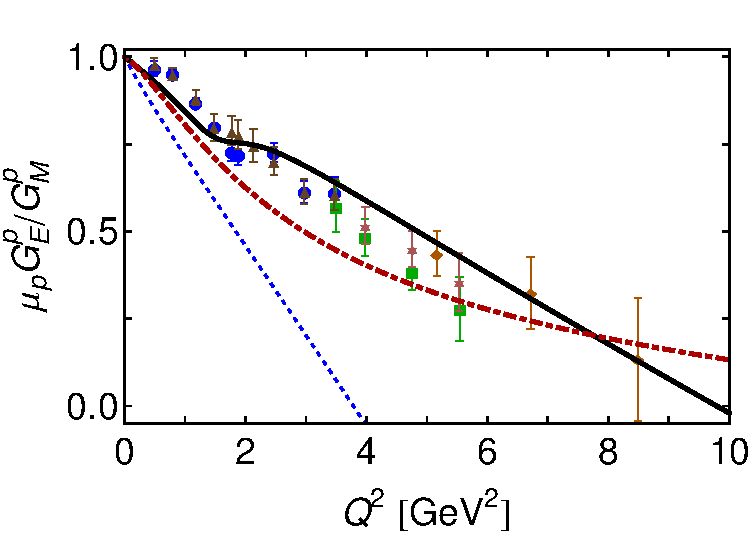
\includegraphics[width = 83 mm]{F3Segovia.pdf}
\caption{Normalized $G_E^p/G_M^p$ \textit{vs.} $Q^2$.  The solid line is the DSE result from~\cite{Segovia:2014aza}, the dash-dot line is the Kelly fit~\cite{kelly04}, and the dotted line is an earlier exploratory DSE result~\cite{Wilson:2011aa}.  The data is from~\cite{jones,gayou:2002,punjabi05A,puckett:2010,puckett:2011}.}
\label{fig:segovia}
\end{center}
\end{figure}
%%%%%%


Qualitatively, the behavior of the form factors in the DSE approach is related to the behavior of the mass function $M(p^2)$.  At lower momenta, where the mass function is far from its perturbative or current quark value, the Pauli form factor is also large compared to its perturbative value and is falling more slowly than perturbation theory predicts.  (For reference, perturbative QCD predicts a $Q^{-4}$ power law falloff for $F_1(Q^2)$ at large $Q^2$, and a $Q^{-6}$ falloff for $F_2(Q^2)$. )  Hence one can get a zero in $G_E(Q^2)$,
\begin{equation}
G_E(Q^2) = F_1(Q^2) - \frac{Q^2}{4 m_p^2} F_2(Q^2)	\,,
\end{equation}
and hence a falloff in the ratio $G_E(Q^2)/G_M(Q^2)$.

For the newer DSE calculations~\cite{Segovia:2014aza}, the zero in $G_E$ is at $Q^2 = 9.5$ GeV$^2$.  If the mass function fell to its low perturbative value more quickly than it does, the quarks would behave more like free quarks, and the value of the Pauli or anomalous magnetic moment, form factor would be small as well as quickly falling.  In such a case, the zero of $G_F(Q^2)$ would be pushed to higher values of $Q^2$ or possibly not occur at all~\cite{Segovia:2014aza}.

%The sources so far consulted do not contain the high $Q^2$ normalization of the form factors,  or detailed direct information about how the quark angular momentum is affecting the form factor results.

We may mention that models based on the Dyson-Schwinger equations do extend to  form factors for other hadronic reactions, such as the electromagnetic $N \to \Delta$ transition~\cite{Segovia:2013uga,Segovia:2014aza}.  The result for the ratio of the electric and magnetic transition form factors for this process, $R_{EM}$, turns out to be small in the DSE approach,  even at momentum transfers above 5 GeV$^2$,  in accord with experimental data.   The perturbative QCD result, that $R_{EM} \to 1$ does ensue, but only at momentum transfers that are extremely high.  %The mechanism that keeps $R_{EM}$ small is not stated in the presentations currently available.




\subsection{Links between Deep-Inelastic Scattering and Nucleon Form Factors}
\label{subsec:dis}

%\subsubsection{Quark Angular Momentum}
%\label{subsubsec:qam}
%

%%%%%%%%%%%%%%%%%
\subsubsection{Perturbative QCD Inspired Models}
\label{subsubsec:pqcd}

%%%%%%%%%%%%%%%%%%

Placeholder text

%%%%%%%%%%%%

\begin{figure}[h]
\centerline{  
  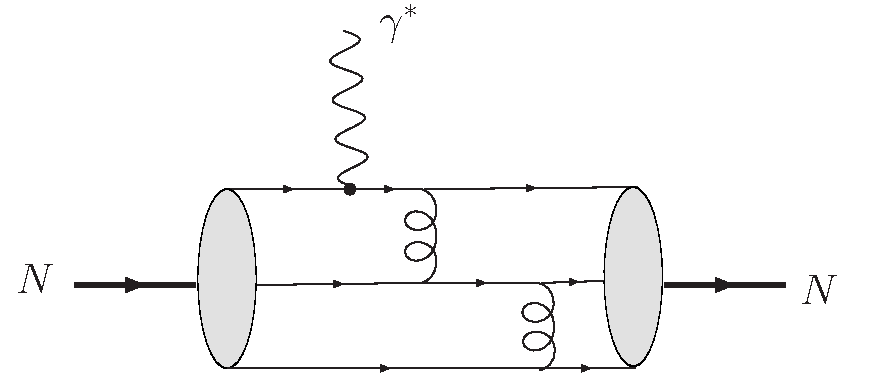
\includegraphics[width = 6 cm]{ff_pqcd.pdf} 
}
\caption{\small Perturbative QCD picture for the nucleon 
e.m. FFs. The highly virtual photon resolves 
the leading three-quark Fock states of the nucleon, described by 
a distribution amplitude. The large momentum is transferred between the quarks 
through two successive gluon exchanges (only one of several possible 
lowest-order diagrams is shown). }
\label{ff_pqcd}
\end{figure}

%%%%%%%%%%

\indent
The nucleon e.m. FFs 
provide a famous test for perturbative QCD. 
Brodsky and Farrar derived scaling rules for dominant helicity amplitudes 
which are expected to be valid at sufficiently high momentum 
transfers $Q^2$~\cite{brodsky}. A photon of sufficient high 
virtuality will see a nucleon consisting of three massless quarks moving 
collinear with the nucleon. 
When measuring an elastic nucleon FF, 
the final state consists again of 
three massless collinear quarks. In order for this (unlikely process) to 
happen, the large momentum of the virtual photon has to be transferred 
among the three quarks through two hard gluon exchanges as illustrated in 
\ref{ff_pqcd}. This hard scattering mechanism is generated by 
valence quark configurations with small transverse size and finite 
light-cone momentum fractions of the total hadron momentum carried by each 
valence quark. The hard amplitude can be written in a factorized 
form~\cite{Chernyak:1977as,Chernyak:1977fk,Efremov:1979qk,brodlep}, 
as a product of a perturbatively calculable hard scattering amplitude and 
two distribution amplitudes (DAs) 
describing how the large longitudinal momentum 
of the initial and final nucleons is shared between their constituents. 
Because each gluon in such hard scattering process carries a virtuality 
proportional to $Q^2$, this leads to the pQCD prediction that the helicity 
conserving nucleon Dirac FF $F_1$ should fall as $1/Q^4$ 
(modulo $\ln Q^2$ factors) at sufficiently high $Q^2$. 
Processes such as in 
\ref{ff_pqcd}, where the interactions among the quarks proceed 
via gluon or photon exchange, both of which are vector interactions, 
conserve the quark helicity in the limit when the quark masses or off-shell 
effects can be neglected. 
In contrast to the helicity conserving FF $F_1$, the nucleon 
Pauli FF $F_2$ involves a helicity flip between the initial and 
final nucleons. Hence it requires one helicity flip at the quark level, which 
is suppressed at large $Q^2$. Therefore, for collinear quarks, i.e. 
moving in a light-cone WF state with 
orbital angular momentum projection 
$l_z = 0$ (along the direction of the fast moving hadron), 
the asymptotic prediction for $F_2$ leads to a 
$1/Q^6$ fall-off at high $Q^2$. 
\newline
\indent
We can test how well the above pQCD scaling predictions for the 
nucleon e.m. FFs 
are satisfied at currently available momentum transfers, see~\ref{scaling}. 
One firstly sees that $F_{1p}$, which has been measured up to about 
30 GeV$^2$, displays an approximate $1/Q^4$ scaling above 10 GeV$^2$. 
For the proton ratio $F_{2 p}/F_{1 p}$, the data up to 5.6 GeV$^2$ show 
no sign of a $1/Q^2$ behavior as predicted by pQCD. 
Instead, the data show that the ratio $F_{2 p}/F_{1 p}$ falls less 
fast than $1/Q^2$ with increasing $Q^2$.
Belitsky, Ji, and Yuan \cite{Belitsky:2002kj} investigated the 
assumption of quarks moving collinearly with the proton, 
underlying the pQCD prediction. 
It has been shown in~\cite{Belitsky:2002kj} that by 
including components in the nucleon light-cone WFs with quark 
orbital angular momentum projection $l_z = 1$, one obtains 
the behavior $F_2/F_1 \to \ln^2 (Q^2 / \Lambda^2)/ Q^2$ at large $Q^2$, 
with $\Lambda$ a non-perturbative mass 
scale~\footnote{In~\cite{jain,Brodsky:2003pw}, 
it has also been discussed that inclusion
  of quark orbital angular momentum yields a ratio $F_{2p}/F_{1p}$ which drops
  less fast than $1/Q^2$ with increasing $Q^2$.  
}. 
Choosing $\Lambda$ around 
$0.3$~GeV, Ref.~\cite{Belitsky:2002kj} noticed that the 
data for $F_{2 p}/F_{1 p}$ support such double-logarithmic enhancement, as 
can be seen from \ref{scaling} (right panel). 
The arguments of~\cite{Belitsky:2002kj} 
still rely on pQCD and it remains to be seen by 
forthcoming data at higher $Q^2$ if this prediction already starts in the 
few GeV$^2$ region. 
%
\begin{figure}[h]
\centerline{  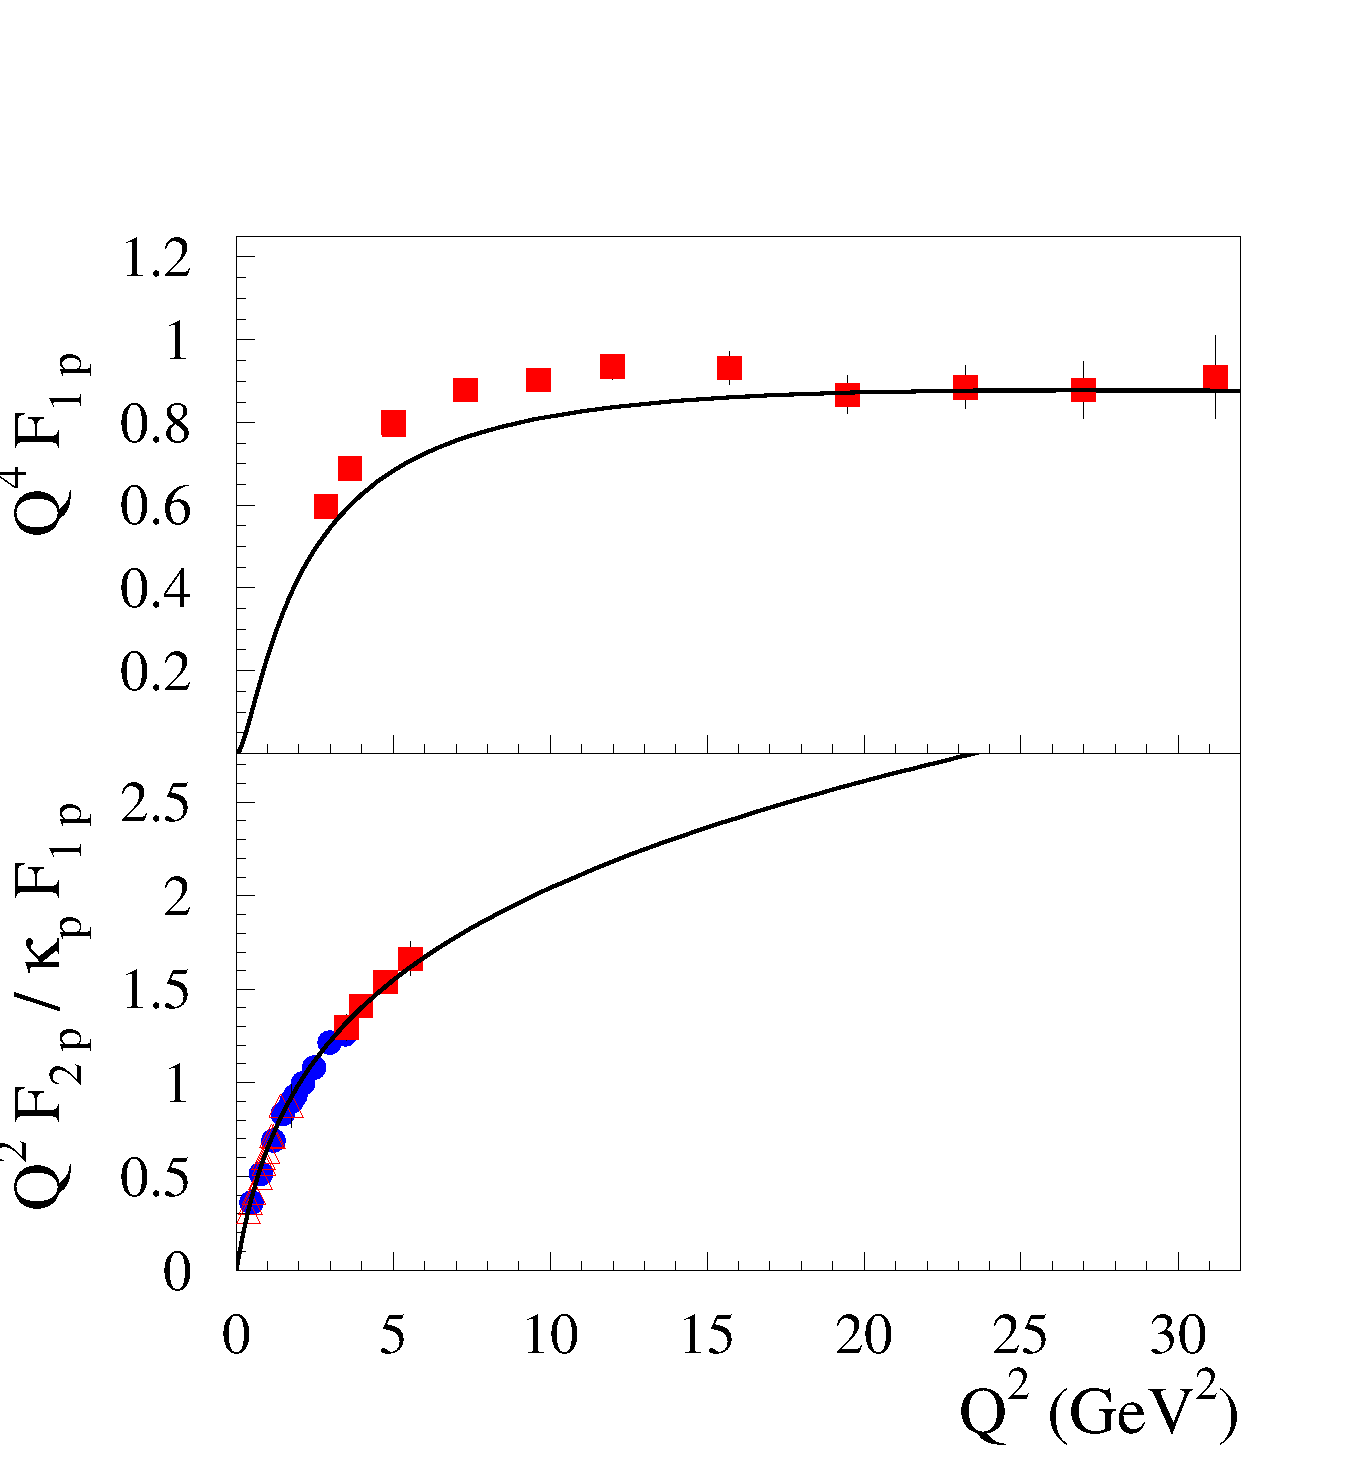
\includegraphics[height = 6 cm ]{f1f2p.pdf}  }

\centerline{  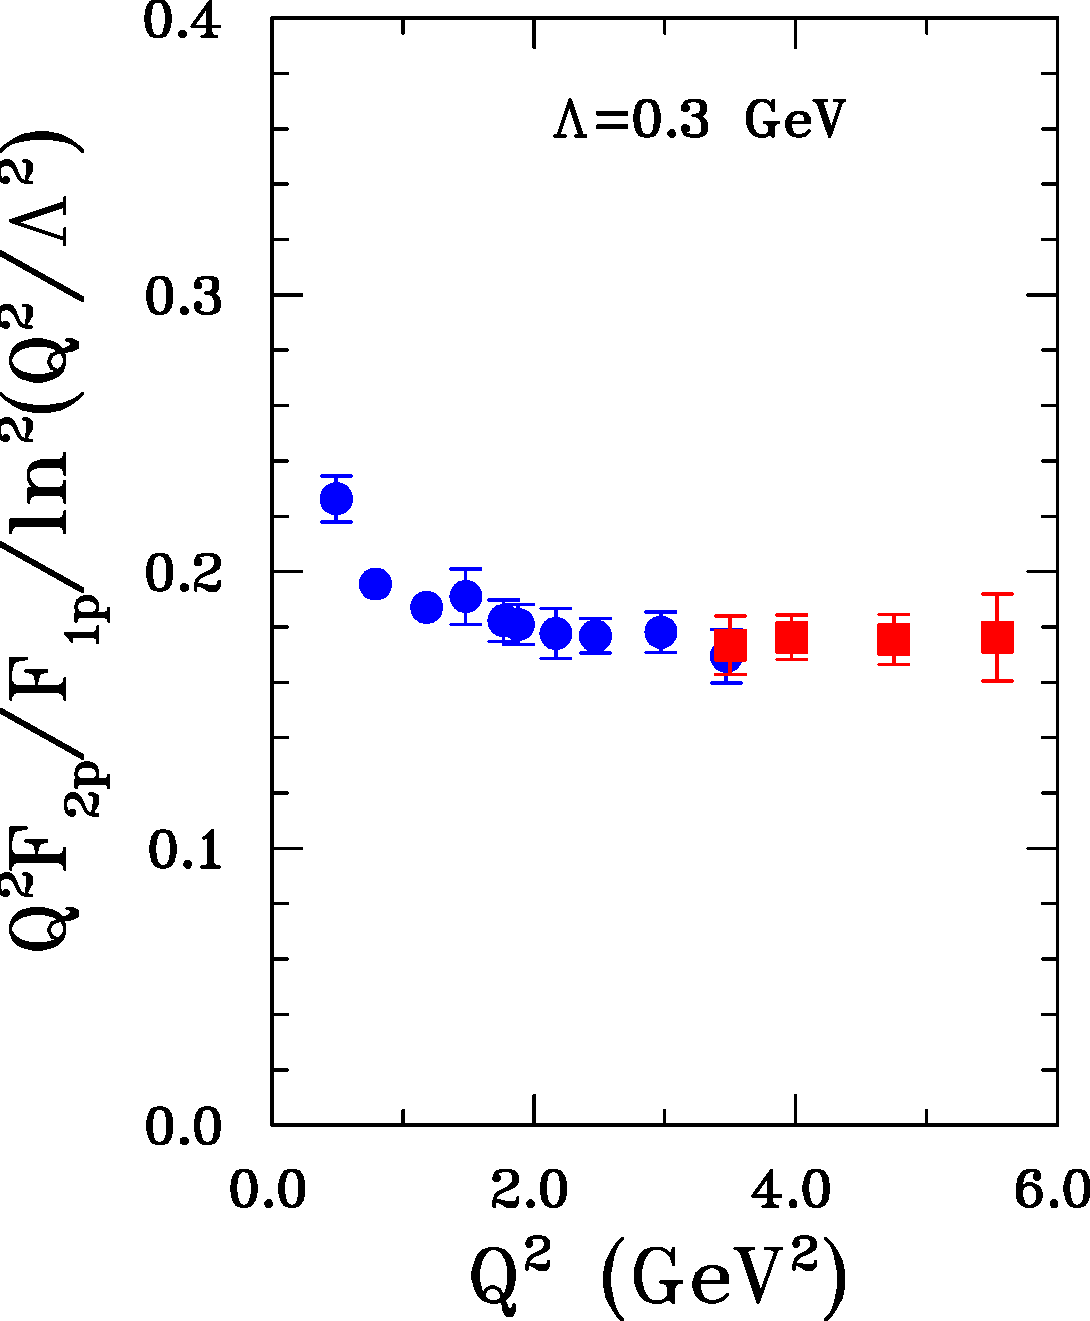
\includegraphics[height = 6 cm]{q2f2f1_belitsky_mod_col.pdf}  }

\caption{\small Test of the scaling behavior of the proton FFs.  
Upper left panel : proton Dirac FF multiplied by $Q^4$.   
Lower left panel : ratio of Pauli to Dirac proton FFs 
multiplied by $Q^2$. 
Right panel : test of the modified scaling prediction for 
$F_{2p}/F_{1p}$ of \cite{Belitsky:2002kj}. 
The data for $F_{1 p}$ are from \cite{sill} (solid squares).  
Data for the ratio $F_{2 p} / F_{1 p}$ on both panels are 
from \cite{punjabi05} (blue solid circles), 
\cite{gayou1} (red open triangles), 
and \cite{gayou2} (red solid squares). 
The curves on the left panels represent the calculation based on the  
three parameter modified Regge GPD parametrization of~\cite{guidal}.}
\label{fig:scaling}
\end{figure}
\newline
\indent
Although at high enough $Q^2$, the pQCD scaling predictions should set in, 
the available data for the nucleon e.m.  
FFs show that one is still far away from this regime. 
Nesterenko and Radyushkin~\cite{Nesterenko:1983ef} argued that the 
above described hard scattering mechanism is suppressed at accessible 
momentum transfers relative to the Feynman mechanism~\cite{feynman}, 
also called soft mechanism. The soft mechanism involves only one active 
quark, and the FF is obtained as an overlap of initial and final 
hadron WFs. 
The hard scattering mechanism on the other hand, 
involving three active quarks, requires the exchange of two gluons, each of 
which brings in a suppression factor $\alpha_s / \pi \sim 0.1$. One therefore 
expects the hard scattering mechanism for $F_{1 p}$  
to be numerically suppressed by a factor 1/100 compared to the soft term, see 
also~\cite{bolz,kroll}. 
Even though the soft mechanism is suppressed asymptotically by a power of 
$1/Q^2$ relative to the hard scattering mechanism, 
it may well dominate at accessible values of $Q^2$.
In~\cite{Nesterenko:1983ef}, the soft contribution 
to the nucleon e.m. FFs was 
estimated using a model based on local quark-hadron duality, and  
was found to yield an approximate $1/Q^4$ behavior 
in the range $Q^2 \sim 10 - 20$~GeV$^2$, 
in qualitative agreement with the $F_{1p}$ data. 
\newline
\indent
In a more recent work, the soft contribution  
was evaluated within the light-cone sum rule (LCSR) approach~\cite{braun06}. 
Using asymptotic DAs for the nucleon, 
the LCSR approach yields values of $G_{Mp}$ and 
$G_{Mn}$ which are within 20 \% compatible with the data in the range 
$Q^2 \sim 1 - 10$~GeV$^2$. The electric FFs however were found to be much
more difficult to describe, with $G_{En}$ overestimated, and 
$G_{Ep}/G_{Mp}$ near constant when using an asymptotic nucleon DA. 
Only when including twist-3 and twist-4 nucleon DAs within a simple model, 
is a qualitative description of the electric
proton and neutron FFs obtained. Such higher twist components hint at the
importance of quark angular momentum components in the nucleon WF. 
\newline
\indent
In Sect.~\ref{theory_gpd}, we have shown that the nucleon 
e.m. FFs can be obtained from model independent 
GPD sum rules. These GPDs, represented by the lower blob in 
\ref{n_dvcs}, are non-perturbative objects which include 
higher Fock components in the nucleon WFs. One 
can use a GPD parametrization to provide an estimate of the soft 
contributions, and expects this non-perturbative approach 
to be relevant in the low and intermediate $Q^2$ region for the FFs.  
This is shown in \ref{scaling} 
(solid curves) from which one sees that the GPD Regge parametrization  
discussed above is able to explain 
at the same time an approximate $1/Q^4$ 
behavior for $F_{1 p}$ and a behavior for $F_{2 p}/F_{1 p}$ 
which falls less steep than $1/Q^2$.  
Forthcoming experiments at the Jefferson Lab 12 GeV facility will extend the 
data for $F_{2 p}/F_{1 p}$ to $Q^2$ values around 
13 GeV$^2$. Such measurements will allow to quantify in detail the higher 
Fock components in the nucleon WF 
(which are all included in the nucleon GPD) versus 
the simple three-quark Fock component, and to map out the 
transition to the perturbative QCD regime. 


%%%%%%%%%%%%%%
\subsubsection{Generalized Parton Distributions}
\label{subsubsec:gpd}

%%%%%%%%%%%%%

Placeholder text


So far we have discussed the $N \to N$ transition 
as revealed with the help of the electromagnetic probe. By measuring 
the response of the hadron to a virtual photon, one measures the matrix 
element of a  well-defined quark-gluon operator (in this case the vector 
operator $\bar q \gamma^\mu q$) over the hadronic state. This matrix element  
can be parametrized in terms of the nucleon e.m. FFs, 
revealing the quark-gluon structure of the nucleon. 
We are however not limited in nature to probes such as photons 
(or $W$, $Z$ bosons for the axial transition). The phenomenon of asymptotic 
freedom of QCD, meaning that at short distances the interactions between 
quarks and gluons become weak, provides us with more sophisticated 
QCD operators to explore the structure of hadrons. Such operators can 
be accessed by selecting a small size configuration of quarks and gluons, 
provided by a hard reaction, such as deep inelastic scattering (DIS), or 
hard exclusive reactions such as deeply virtual Compton scattering (DVCS).  
We will be mostly interested here in DVCS reactions which are of the type 
$\gamma^*(q_h) + N(p) \to \gamma(q^\prime) + N(p^\prime)$, where the 
virtual photon momentum $q_h$ is the hard scale. 
The common important feature of such hard reactions is the possibility
to separate clearly the perturbative and nonperturbative stages of
the interactions~: this is the so-called factorization property. 
\newline
\indent
The all-order factorization theorem for the DVCS process on the 
nucleon has been proven in~\cite{Ji98a,Col99,rady}.
Qualitatively one can say that the hard reactions allow
one to perform a ``microsurgery'' of a nucleon by removing in a
controlled way a quark of one flavor and spin and implanting
instead another quark in the final nucleon. 
It is illustrated in \ref{n_dvcs} 
for the case of the DVCS process. 
The non-perturbative stage of such hard exclusive 
electroproduction processes is described by 
universal objects, so-called generalized parton distributions 
(GPDs)~\cite{Muller:1998fv,ji,Radyushkin:1996nd}, 
see~\cite{Ji:1998pc,Goeke:2001tz,Diehl:2003ny,Belitsky:2005qn,Ji:2004gf} 
for reviews and references. 
\newline
\indent
The nucleon structure information entering the nucleon DVCS process, 
can be parametrized at leading twist-2 level, in
terms of four quark chirality conserving GPDs. 
The GPDs depend on three variables: the quark longitudinal 
momentum fractions $x$ and $\xi$, and the momentum transfer 
$Q^2 = - q^2$ to the nucleon.
The light-cone momentum fraction $x$ is defined by $k^+ = x P^+$,
where $k$ is the quark loop momentum and
$P$ is the average nucleon momentum 
$P = (p + p^{\ \prime})/2$, where $p (p^{\ \prime})$
are the initial (final) nucleon four-momenta respectively,  
see \ref{n_dvcs}.
The skewedness variable $\xi$ is
defined by $q^+ = - 2 \xi \,P^+$, where 
$q = p^{\ \prime} - p$ is the
overall momentum transfer in the process, and where
$2 \xi \rightarrow x_B/(1 - x_B/2)$ in the Bjorken limit: 
$x_B = Q_h^2/(2 p \cdot q_h)$ is the usual Bjorken scaling variable, 
with $Q_h^2 = -q_h^2 > 0$ the virtuality of the hard photon.
\newline
\indent
The DVCS process 
corresponds to the kinematics $Q_h^2 \gg Q^2, M^2$, 
so that at twist-2 level, terms proportional to $Q^2 / Q_h^2$ 
or $M^2 / Q_h^2$ are neglected in the amplitude.  
In a frame where the virtual photon momentum \( q_h^{\mu } \) and the average
nucleon momentum \(  P^{\mu } \) are collinear
along the \( z \)-axis and in opposite directions, one can parameterize
the non-perturbative object entering the nucleon DVCS process as 
(following Ji~\cite{ji})\footnote{In all non-local
expressions we always assume the gauge link:
P$\exp(ig\int dx^\mu A_\mu)$, ensuring the color gauge
invariance.}:
\begin{eqnarray}
&& \frac{1}{2\pi} \, \int dy^{-}e^{ix  P^{+}y^{-}}
		\nonumber\\
&& \qquad		\times
\left. \langle N(p^\prime)|\bar{\psi } (-y/2) \; \gamma \cdot n \; \psi (y/2)
| N(p) \rangle \right|_{y^{+}=\vec{y}_{\perp }=0} 
						\nonumber \\
&&=\; H^{q}(x,\xi ,Q^2)\; \bar{N}(p^{'}) \; \gamma \cdot n \; N(p)
						\nonumber\\
&& \qquad
+ \  E^{q}(x,\xi ,Q^2)\; \bar{N}(p^{'}) \; i\sigma^{\mu \nu} 
\frac{n_\mu \, q_\nu}{2 M} \; N(p) ,
\label{eq:qsplitting}
\end{eqnarray}
where \( \psi  \) is the quark field
of flavor $q$, \( N \) the nucleon spinor, and $n^\mu$ is a 
light-cone vector along the negative $z$-direction. 
The {\it lhs} of Eq.~(\ref{eq:qsplitting}) can be interpreted as a Fourier
integral along the light-cone distance $y^-$ of a quark-quark
correlation function, representing the process where
a quark is taken out of the
initial nucleon (having momentum $p$) at the space-time point $y/2$, and
is put back in the final nucleon (having momentum $p^{\ \prime}$) 
at the space-time
point $-y/2$. This process takes place at equal light-cone time ($y^+
= 0$) and at zero transverse separation ($\vec y_\perp = 0$) between
the quarks. The resulting one-dimensional Fourier integral along the
light-cone distance $y^-$ is with respect to the quark light-cone
momentum $x  P^+$.
The {\it rhs} of Eq.~(\ref{eq:qsplitting}) parametrizes this
non-perturbative object in terms of the GPDs $H^q$ and $E^q$ 
for a quark of flavor $q$.  
The quark vector operator ($\gamma \cdot n$) 
corresponds at the nucleon side to a vector transition 
(parametrized by the function $H^q$) and
a tensor transition (parametrized by the function $E^q$). 
Analogously, there are two GPDs corresponding to 
a quark axial vector operator ($\gamma \cdot n \gamma_5$), which are 
commonly denoted by the polarized GPDs $\tilde H^q$ and $\tilde E^q$. 

%%%%%%%%
\begin{figure}[t]
\centerline{  
  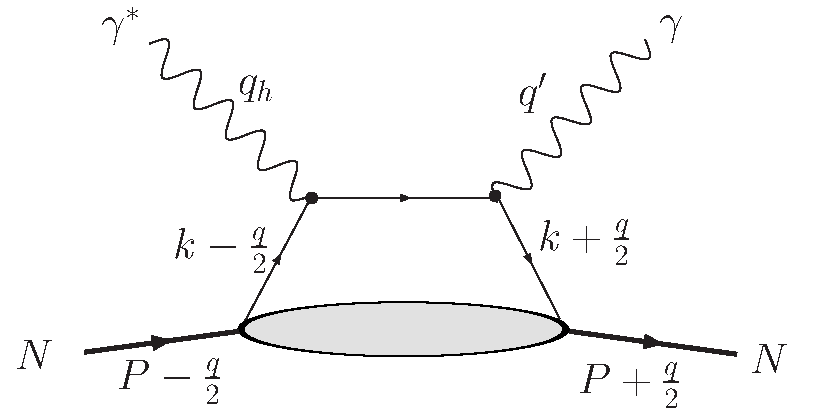
\includegraphics[width = 6 cm]{n_dvcs.pdf} 
}
\caption{\small 
The ``handbag'' diagram for the nucleon DVCS process. 
Provided the virtuality of the initial photon (with momentum $q_h$) 
is sufficiently large, the 
QCD factorization theorem allows to express the 
total amplitude as the convolution  
of a Compton process at the quark level and a non-perturbative 
amplitude parameterized in terms of generalized parton distributions 
(lower blob). The diagram with the photon lines crossed is also understood.    
}
\label{n_dvcs}
\end{figure}
%%%%%%%%

%\newline
\indent
The variable $x$ in the GPDs runs from $-1$ to 1.
Therefore, the momentum fractions of the
active quarks ($x + \xi$) for the initial quark and ($x - \xi$) for the final 
quark can either be positive or negative. Since positive
(negative) momentum fractions correspond to quarks (antiquarks), it
has been noted in \cite{Radyushkin:1996nd} that in this way, one can
identify two regions for the GPDs:
when $x > \xi$ both partons represent quarks, whereas for
$x < - \xi$ both partons represent antiquarks. In these regions,
the GPDs are the generalizations of the usual parton distributions from
DIS. Actually, in the forward direction, the GPD $H$ 
reduces to the quark (anti-quark) density distribution $q(x)$ 
($\bar q(x)$) obtained from DIS: 
$H^q(x,0,0) = q(x)$, for $x > 0$;  
$H^q(x,0,0) = - \bar q(-x)$, for $x < 0$. 
The GPD $E$ 
is not measurable through DIS because the associated tensor 
in Eq.~(\ref{eq:qsplitting}) vanishes in the forward limit ($q \to 0$).
Therefore, $E$ is a new leading twist function, which
is accessible by measuring hard exclusive electroproduction reactions, such 
as DVCS.
\newline
\indent
Besides coinciding with the quark distributions at vanishing momentum
transfer, the GPDs have interesting links with other
nucleon structure quantities. The first moments of the GPDs are related to
the elastic FFs
of the nucleon through model independent sum rules.
By integrating Eq.~(\ref{eq:qsplitting}) over \( x \), one
obtains for any $\xi$
the following relations for a particular quark flavor \cite{ji} :
\begin{eqnarray}
\int_{-1}^{+1}dx\, H^{q}(x,\xi ,Q^2)&=& F_{1}^{q}(Q^2)\, ,
				\nonumber\\
\int _{-1}^{+1}dx\, E^{q}(x,\xi ,Q^2)&=& F_{2}^{q}(Q^2)\, ,
\label{eq:ffsumrulehe}
\end{eqnarray}
where $F_1^q$ ($F_2^q$) represents the elastic Dirac (Pauli) FFs for the
 quark flavor $q$ in the nucleon. These quark FFs are expressed, 
using $SU(2)$ isospin, 
as flavor combinations of the proton and neutron elastic FFs as:
\begin{eqnarray}
F_{1}^u &=& 2\,F_{1 p}\,+\,F_{1 n}\,+\,F_{1}^{s}\; , 
			\nonumber\\
F_{1}^d &=&, 2\,F_{1 n}\,+\,F_{1 p}\,+\,F_{1}^{s}\; ,
\label{eq:vecff}
\end{eqnarray}
where $F_{1}^{s}$ 
is the strangeness FF of the nucleon (which is neglected in 
the calculations discussed below).
Relations similar to Eq.~(\ref{eq:vecff}) hold for the
Pauli FFs \( F_{2}^{q} \).
At $Q^2 = 0$, the normalizations of the Dirac FFs are given by:
$F_{1}^{u}(0) = 2$ ($F_{1}^{d}(0) = 1$) 
so as to yield the normalization of 2 (1) for the
$u$ ($d$)-quark distributions in the proton. 
The normalizations of the Pauli FF at $Q^2 = 0$ are 
given by $F_{2}^{q}(0) = \kappa^q$ (for $q = u, d$), where 
$\kappa^u, \kappa^d$ can be expressed 
in terms of the proton ($\kappa_p$) 
and neutron ($\kappa_n$) anomalous magnetic moments as:
\begin{eqnarray}
\kappa^u &\equiv & 2 \kappa_p + \kappa_n = +1.673, 
			\nonumber\\
\kappa^d&\equiv & \kappa_p + 2 \kappa_n = -2.033. 
\label{eq:kappaud}
\end{eqnarray}
\indent
The above sum rules allow us to make a prediction for the 
nucleon e.m. FFs provided we have a model for the nucleon GPDs. 
Note that the sum rules of Eq.~(\ref{eq:ffsumrulehe}) only involve valence 
quark GPDs, since the sea-quark and anti-quark contributions 
cancel each other in the sum rules. 
Since the results of the integration 
in Eq.~(\ref{eq:ffsumrulehe}) do not depend on the skewness 
$\xi$~\footnote{This is the simplest example
of a so-called polynomiality condition when calculating moments of GPDs.}, one 
can choose $\xi = 0$ in these sum rules. We therefore only discuss 
the GPDs $H$ and $E$ at $\xi = 0$ in the following. 
\newline
\indent 
In~\cite{diehl,guidal}, parameterizations of GPDs were developed 
which have a Regge behavior at small $x$ and $Q^2$, and which were 
modified to larger $Q^2$ behavior so as to lead to the observed power 
behavior of the FFs~\cite{Burkardt:2002hr,Burkardt:2004bv}. 
A modified Regge parameterization for $H$ and $E$ was proposed in 
\cite{guidal}~:
\begin{eqnarray}
H^q (x,0,Q^2) &=& q_v (x)\,  x^{\alpha^\prime \, (1 - x) \, Q^2}, 
			\nonumber\\
E^q (x, 0, Q^2) &=& \frac{\kappa^q}{N^q} 
\, (1 - x)^{\eta^q} \, q_v(x) \, 
{{x^{\alpha' \, (1 - x) \, Q^2}}} \, , 
\label{eq:gpd_r2}
\end{eqnarray}
depending on 3 parameters.  
The Regge slope $\alpha^\prime$ is determined from the Dirac radius, 
and two parameters $\eta^u$ and $\eta^d$, entering the GPD $E$, ensure that 
the $x\sim 1 $ limit of $E^q$ 
has extra powers of $1-x$ compared to that  of $H^q$. 
This results in a proton helicity flip FF $F_2$ which has a faster 
power fall-off at large $Q^2$ than $F_1$, as observed experimentally.   
Furthermore, in Eq.~(\ref{eq:gpd_r2}), 
the normalization factors $N^u$ and $N^d$ are given by~:  
\begin{eqnarray}
N^u &=&  \int _{0}^{1}dx \; (1 - x)^{\eta^u} \, u_v(x) \, ,
		\nonumber\\
N^d &=&  \int _{0}^{1}dx \; (1 - x)^{\eta^d} \, d_v(x) \, ,
\label{eq:nd}  
\end{eqnarray} 
and guarantee the normalization condition for the GPD $E^q$. 
%\newline
\indent
Diehl {\it et al.}~\cite{diehl} chose a more 
general functional form for $E^q$ at the expense of more free parameters. 
In the following, we discuss the `minimal' model with 3 parameters, 
and refer the interested reader to~\cite{diehl} for a study of more 
general functional forms. 
The 3 free parameters in the resulting modified Regge ansatz 
are to be determined from a fit to the FF data. 


%%%%%%%%%%%%%%%%

\begin{figure}[t]
\begin{center}
%\vspace{-1.2cm}
%\hspace{1cm}
  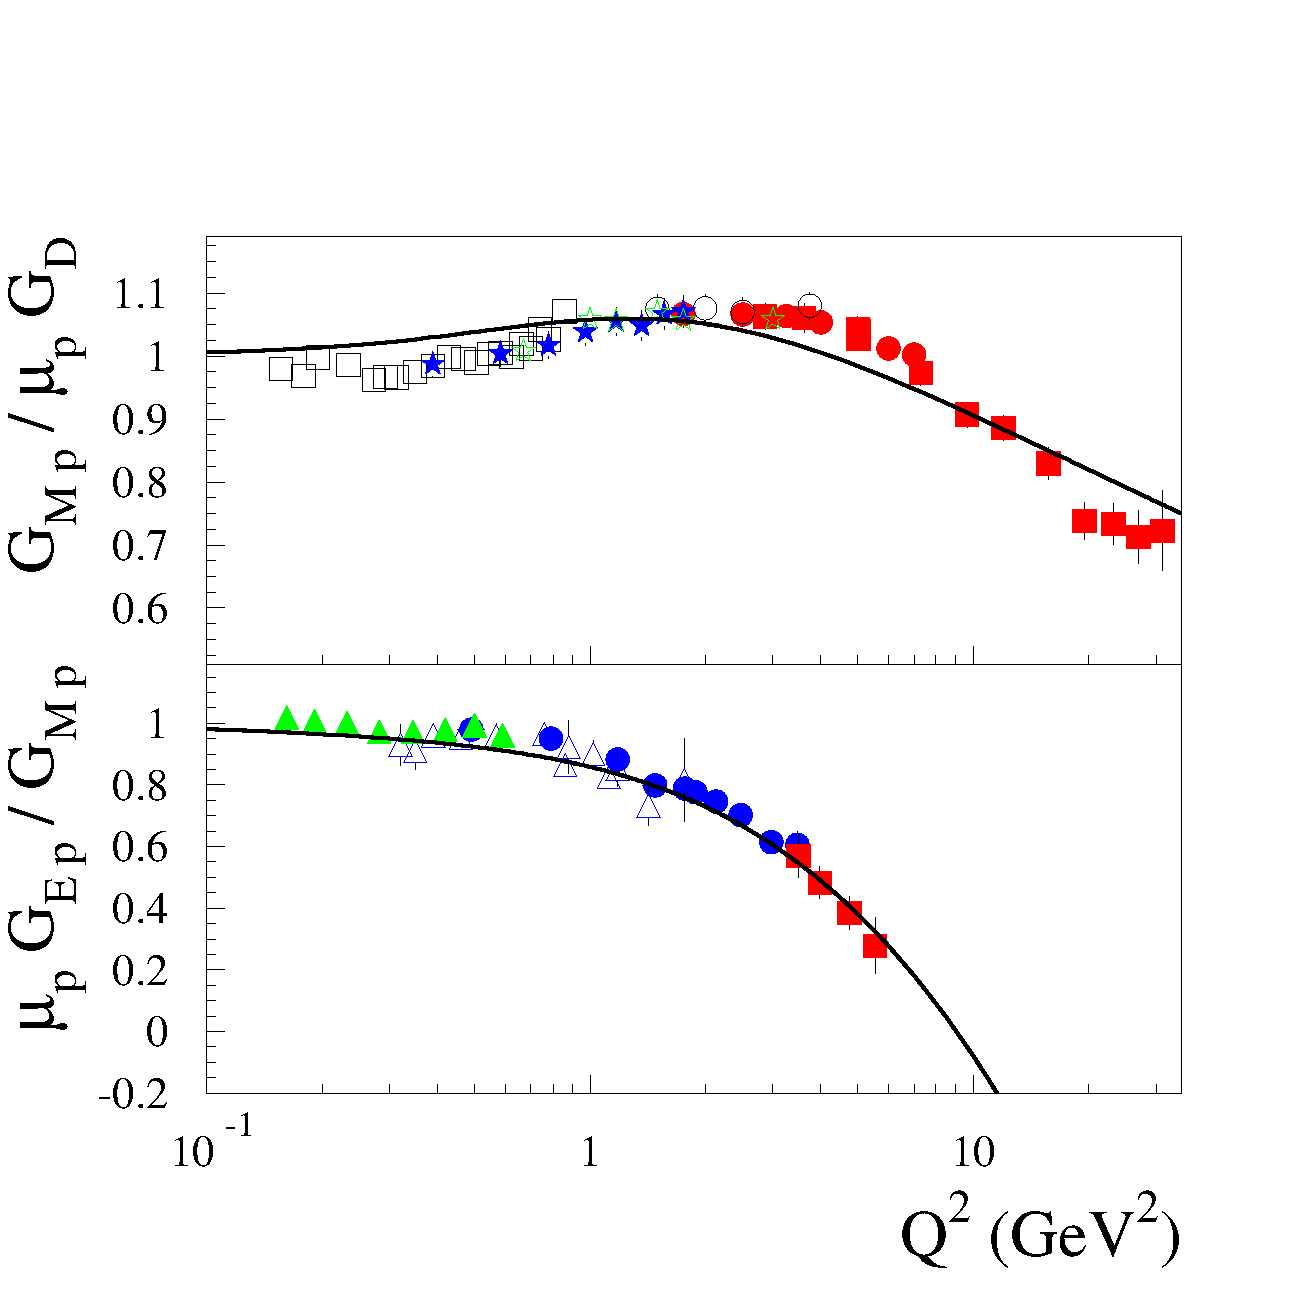
\includegraphics[width = 6.5 cm]{gegmproton_col.pdf}
  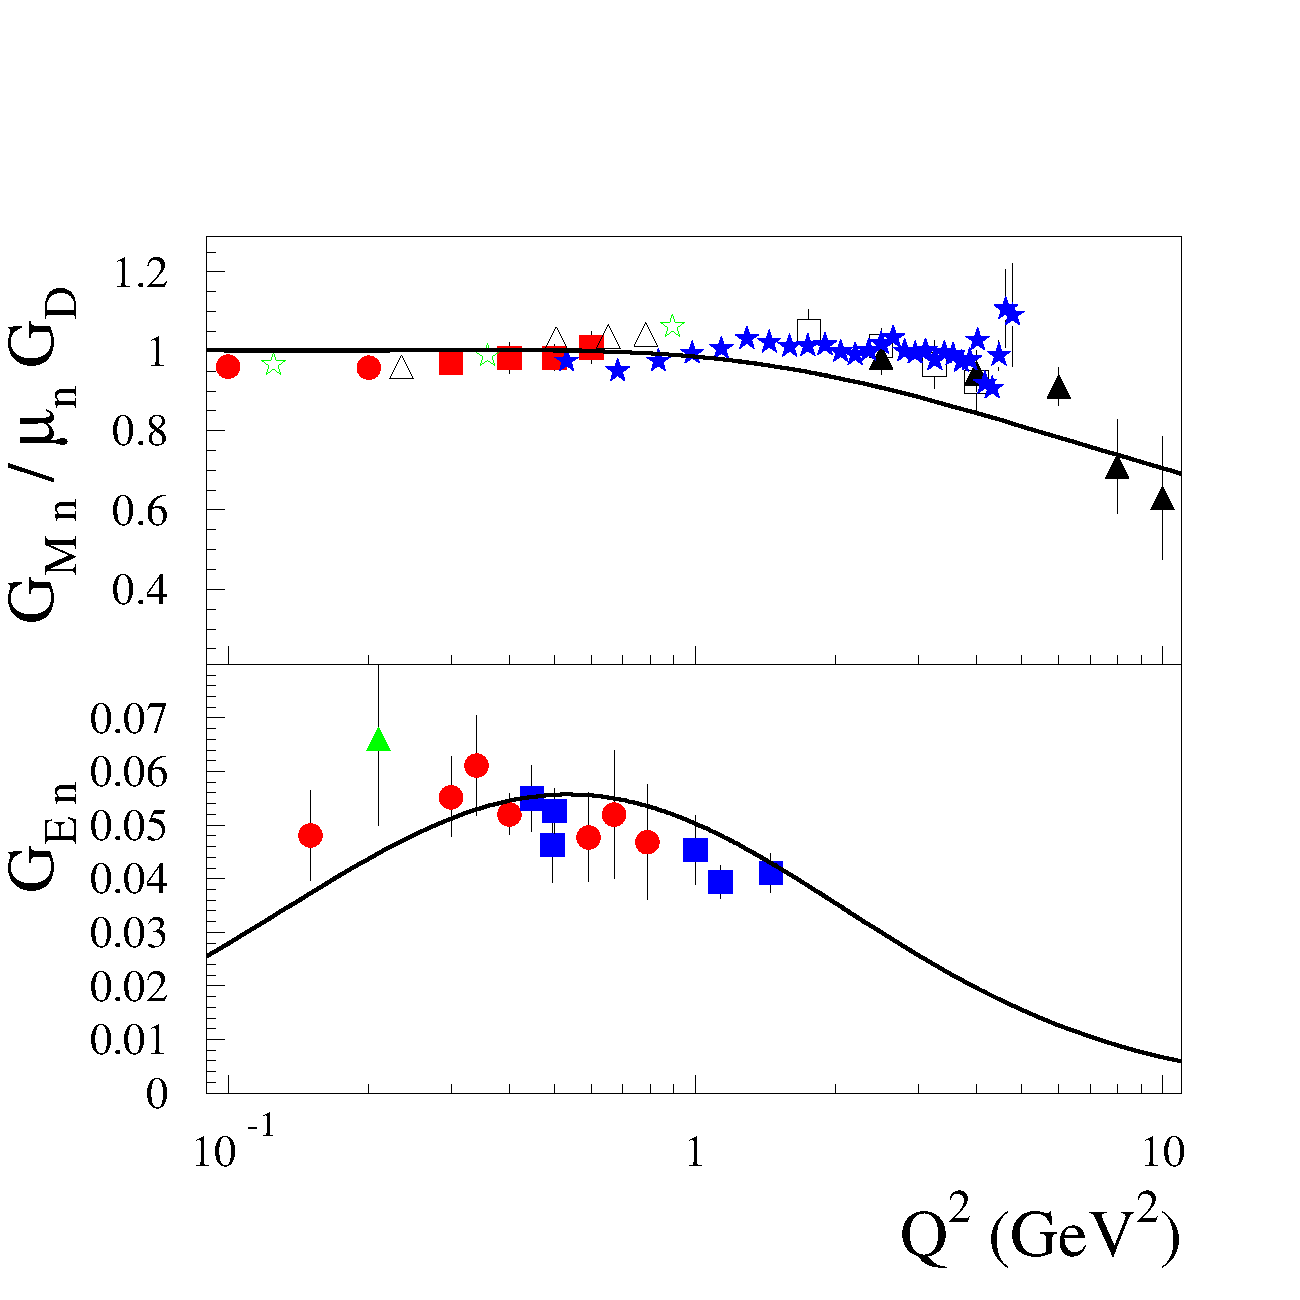
\includegraphics[width = 6.5 cm]{gegmneutron_col.pdf}
\caption{\small GPD calculation of 
$G_{Mp}$ and $G_{Mn}$ relative to the dipole $G_D$ (upper panels), 
ratio of $G_{Ep}/G_{Mp}$ (lower left panel), 
and $G_{En}$ (lower right panel), according to Ref.~\cite{guidal}. 
The curves are a 3 parameter modified Regge parameterization : 
$\alpha^\prime = 1.105$\, GeV$^{-2}$, $\eta^u$ = 1.713 and $\eta^d$ = 0.566. 
Data for $G_{M p}$ are from   
\cite{janssens} (open squares), \cite{litt} (open circles),
\cite{berger} (blue solid stars), \cite{bartel} (green open stars), 
\cite{andivahis} (red solid circles), \cite{sill} 
(red solid squares), 
according to the recent re-analysis of Ref.~\cite{brash}. 
Data for the ratio $G_{E p} / G_{M p}$ are from 
\cite{gayou1} (blue open triangles), 
\cite{gayou2} (red solid squares),
\cite{punjabi05} (blue solid circles), 
and \cite{crawford} (green solid triangles). 
The data for $G_{M n}$ are from 
\cite{xu00} (red solid circles), 
\cite{xu02} (red solid squares),    
\cite{anklin2} (open triangles), \cite{kubon} (green open stars), 
\cite{lung} (open squares), \cite{rock} (solid triangles), 
and \cite{brooks} (blue solid stars).
The data for $G_{E n}$ are from 
double polarization experiments at 
MAMI~\cite{herberg,ostrick,becker,rohe,glazier} (red solid circles), 
NIKHEF~\cite{passchier} (green solid triangle),  
and JLab~\cite{zhu,madey,warren} (blue solid squares). 
}
\label{fig:gegmpn}
\end{center}
\end{figure}

%%%%%%%%%%%

In Fig.~\ref{fig:gegmpn}, the proton and neutron Sachs electric 
and magnetic FFs are shown. 
One observes that the 3-parameter 
modified Regge model gives a rather good overall 
description of the available FF data for both proton and neutron 
in the whole $Q^2$ range,   
using as value for the Regge trajectory 
$\alpha^\prime $ = 1.105 \,GeV$^{-2}$, 
and the following values for the coefficients 
governing the $x \to 1$ behavior of the $E$-type GPDs:  
$\eta^u$ = 1.713 and $\eta^d$ = 0.566.  
Note that a value $\eta^q = 2$ 
corresponds to a $ 1/Q^2$ asymptotic behavior of the ratio
$F_2^q / F_1^q$ at large $Q^2$. 
The modified Regge GPD parameterization allows 
to accurately describe the decreasing ratio of $G_{E p} / G_{M p}$ 
with increasing $Q^2$, and 
also leads to a zero for $G_{E p}$ at a 
momentum transfer of $Q^2 \simeq 8$~GeV$^2$, which will be within the range 
covered by an upcoming JLab experiment~\cite{E-04-108}. 





%%%%%%%%%%%%%%%%%%
\subsection{Lattice QCD Calculations of Nucleon Form Factors}
\label{subsec:lattice}
%%%%%%%%%%%%%%%%%%

Strictly speaking, lattice calculations of nucleon form factors are currently available only for the isovector form factors.  

Isoscalar form factors require calculations of disconnected diagrams, which are diagrams with quark loops not connected to the quark lines emanating from or ending on the lattice nucleon source or sink.  There are gluons that attach the quark loops to the valence quarks, but these are not indicated in lattice diagrams, hence the phrase ``disconnected.''  Contributions from the disconnected loops require computer time intensive calculations, and the calculations remain undone.  However, the disconnected diagrams contribute equally to proton and neutron, so the isovector case can be considered without them.  

A review including lattice form factor results up to 2010 is available in~\cite{Hagler:2009ni}, and newer lattice form factor results are reported in~\cite{Alexandrou:2013joa,Bhattacharya:2013ehc,Green:2014xba}.


The new calculations have pion masses from 373 MeV down to a close to physical 149 MeV in~\cite{Green:2014xba}.  The latter also strove to reduce contamination from excited nucleons.  They analyze their lattice data using three methods which they call the standard ratio method, the summation method, and the generalized pencil-of-function method (GPoF), with varying outcomes.  The best results, judged by comparison to data as represented by one of the standard fits~\cite{Alberico:2008sz}, come from the summation method.  Here agreement with experimental data is good for both $G_E^v$ and $G_M^v$ in the region considered, which is $Q^2$ from scattering threshold up to about 0.5 GeV$^2$, with uncertainty limits about $20\%$ at $Q^2$ of $0.4$ GeV$^2$,

Refs.~\cite{Alexandrou:2013joa,Bhattacharya:2013ehc} have pion masses in the 213--373 MeV range, and quote results for somewhat higher $Q^2$.  For $Q^2$ above about $0.6$ GeV$^2$, their isovector form factors results tend to be 50\% or so above the data for $G_E^v$ (or $F_1^v$), with uncertainties indicated at about 10\%.  For $G_M^v$ (or $F_2^v$) the results are closer to data .  The authors of these works do point out that the lattice treatments with these pion masses are all consistent with each other.

One may specifically focus on nucleon radii calculated from lattice gauge theory.  In the future, it may be possible and desirable to calculate using a dedicated correlator which gives directly the slope of the form factor at zero momentum transfer.  Finding such correlators by taking derivatives of known correlators is suggested and studied~\cite{deDivitiis:2012vs} for lattice calculations of form factors at points where the Lorentz factors they multiply go to zero.  Applications in~\cite{deDivitiis:2012vs} are to form factors for semi-leptonic scalar meson decay, and to hadronic vacuum polarization corrections to the muon $(g-2)$.

At present, lattice calculations of nucleon radii proceed by calculating the form factor at several non-zero $Q^2$, fitting to a suitable form, typically a dipole form, and finding the radius by extrapolating to zero $Q^2$.  Truly complete results are available only for the isovector nucleon.  Ref.~\cite{Green:2014xba} presents a plot of radius results for lattice calculations at various pion masses.  They use the Dirac radius, obtained from the slope of $F_1^v$, rather than the charge radius, but these are related by, using the proton as an example,
\begin{equation}
\langle r_{1p}^2 \rangle = \langle r_{Ep}^2 \rangle - \frac{3}{2} \frac{\kappa_p}{m_p^2}	\,.
\end{equation}
Hence, given the great accuracy of the magnetic moment measurements, one knows the Dirac radii to the same accuracy as the charge radii.  

The great interest is obtain sufficient accuracy from the lattice results to be able to adjudicate between the electron and muon measured values of the isovector charge or Dirac radii.  The electron measured isovector radius is straightforward to look up, the muon measured value of the Dirac or charge radius is for now a defined quantity obtained by using the electron value for the neutron radius-squared.  Using the summation method, Ref.~\cite{Green:2014xba} obtain, by extrapolation to the physical pion mass, a value of the isovector Dirac radius between the muonic and electronic results, with uncertainties that accommodate both at about the one standard deviation level.  However, using the GPoF or ratio method gives a smaller $\langle r_{1}^2 \rangle^v$, on the order of $2/3$ the value from the summation method.

One may say there opportunity for further work.  An uncertainty of 1\% or less for the proton alone is needed for a lattice calculation to impact the proton radius puzzle.







%\begin{thebibliography}{PPV06}

@article{hofs53,
author={R. Hofstadter, H.R. Fechter and J.A. McIntyre,
Phys. Rev.  
92 
(1953) 
978.

@article{hofs55,
author={R. Hofstadter and R.W. McAllister, 
Phys. Rev. 
98 
(1955) 
217.

@article{yearian, 
author={M.R. Yearian and R. Hofstadter, 
Phys. Rev. 
110 
(1958) 
552.

@article{rosenbluth, 
author={M.N. Rosenbluth, 
Phys. Rev.  
79 
(1950) 
615.

@article{jones,
author={M.K. Jones, {\it et al.}, Jefferson Lab Hall A Collaboration,
Phys.\ Rev.\ Lett.\ 
84 
(2000) 
1398.

@article{gayou2, 
author={O. Gayou, {\it et al.}, Jefferson Lab Hall A Collaboration,
Phys.\ Rev.\ Lett.\ 
88 
(2002) 
092301.

@article{punjabi05, 
author={V. Punjabi, {\it et al.},
  Phys.\ Rev.\ C  
71 
(2005) 
055202;


@article{punjabi05err, 
author={V. Punjabi, {\it et al.},
Phys.\ Rev.\ C 
71 
(2005)  
069902 (erratum).

@article{gao1,
author={  H.Y.Gao,
  Int.\ J.\ Mod.\ Phys.\ E 
12 
(2003) 
1.

@article{gao2,
author={  H.Y.Gao, 
Int.\ J.\ Mod.\ Phys.\ E 
12 
(2003) 
567 (erratum).

@article{charleskees, 
author={  C.E. Hyde-Wright, K.~de Jager,
  Ann.\ Rev.\ Nucl.\ Part.\ Sci.\  
54 
(2004) 
217.

@article{arrreview,
author={J. Arrington, C.D. Roberts, J.M. Zanotti, 
arXiv:nucl-th/0611050 
2006.

@article{Baldini:2005vn,
author={R. Baldini, M.~Mirazita, S.~Pacetti, C.~Bini, P.~Gauzzi, M.~Negrini,
  Nucl.\ Phys.\  A 
  755, 
  (2005) 
  286.

@article{Beise:2004py,
author={  E.J. Beise, M.L.~Pitt, D.T.~Spayde,
  Prog.\ Part.\ Nucl.\ Phys.\  
  54 
  (2005) 
  289.

@article{rose,
author={M.E. Rose, 
Phys. Rev. 
73 
(1947) 
279.

@article{hofstad53,
author={R. Hofstadter, H.R. Fechter, J.A. McIntyre,
Phys. Rev.  
91 
(1953) 
422.

@article{hofst56,
author={R. Hofstadter, 
Rev. Mod. Phys. 
28 
(1956) 
214.

@article{stern,
author={O. Stern, 
Nature  
132 
(1933) 
103.

@article{schiff,
author={L.I. Schiff,
 Stanford Microwave Laboratory, 
 report no. 102, 
 (1949) 
 (unpublished).

@article{mcallis56, 
author={R.W. McAllister, R. Hofstadter, 
Phys. Rev. 
102 
(1956) 
851.

@article{hofst58,
author={R. Hofstadter, F. Bumiller, M.R. Yearian, 
Rev. Mod. Phys.  
30 
(1958) 
482. 

@article{clementel, 
author={E. Clementel, C. Villi, 
Nuov. Cim  
4 
(1956) 
1207.

@article{rekalo, 
author={M.P. Rekalo, E. Tomasi-Gustafsson, 
arXiv:nucl-th/0202025, 
2002.

@article{foldy52, 
author={L.L. Foldy, 
Phys. Rev.  
87 
(1952) 
688.

@article{guichon,
author={  P.A.M. Guichon, M.~Vanderhaeghen,
  Phys.\ Rev.\ Lett.\   
  91 
  (2003) 
  142303.

@article{hofst60, 
author={R. Hofstadter, 
Proc. of 9$^{th}$ Intern. Ann. Conference on High Energy Physics Academy of Science USSR, Moscow, 
I
1960, 
 355.

@article{bumiller, 
author={F. Bumiller, M. Croissiaux, R. Hofstadter, 
Phys. Rev. Lett.  
5 
(1960) 
261;  
R. Hofstadter, F. Bumiller, M. Croissiaux,  
Phys. Rev. Lett.  
5 
(1960) 
263.

@article{yennie57, 
author={D.R. Yennie, M.M. L\'evy, D.G. Ravenhall, 
Rev. Mod. Phys.  
29 
(1957) 
144.

@article{ernst,
author={F.J. Ernst, R.G. Sachs, K.C. Wali, 
Phys. Rev. 
119 
(1960) 
1105. 

@article{walecka, 
author={J.D. Walecka, 
Nuovo Cimento  
11 
(1959) 
821.

@article{hand63, 
author={L.N. Hand, D.G. Miller, R. Wilson, 
Rev. Mod. Phys. 
35 
(1963) 
335. 

@article{kelly02,
author={J.J. Kelly,  
Phys. Rev. C 
66 
(2002) 
065203.

@article{wilsonrr,
author={  R.R. Wilson, J.S.~Levinger,
  Ann.\ Rev.\ Nucl.\ Part.\ Sci.\  
  14 
  (1964) 
  135.

@article{berger, 
author={Ch. Berger, {\it et al.}, 
Phys. Lett. 
B  
35 
(1971) 
87.

@article{bartel, 
author={W. Bartel, {\it et al.},
Nucl.\ Phys.\ B  
58 
(1973) 
429.

@article{andivahis, 
author={L. Andivahis, {\it et al.},
Phys.\ Rev.\ D  
50, 
(1994) 
5491

@article{bosted1,
P.~E. Bosted, {\it et al}, 
Phys. Rev. Lett.  
68 
(1992) 
3841. 

@article{price, 
L.E. Price, {\it et al.}, 
Phys. Rev. D  
4 
(1971) 
45.

@article{hanson, 
K.M. Hanson, {\it et al.}, 
Phys. Rev. D  
8 
(1973) 
753.

@article{litt, 
J. Litt, {\it et al.}, 
Phys. Lett. B  
31 
(1970) 
40.

@article{iach,
F. Iachello, A.D. Jackson, A. Land\'e, 
Phys. Lett. B  
43 
(1973) 
191. 

@article{hohler,  
G. H\"ohler, {\it et al.}, 
Nucl. Phys. B  
114 
(1976) 
505.

@article{gari1,  
M.F. Gari, W. Kr\"umpelmann, 
Z. Phys. A  
322 
(1985) 
689; 

@article{gar2,
M.F. Gari, W. Kr\"umpelmann, 
Phys. Lett. B  
274 
(1992) 
150

@article{gar3,
M.F. Gari, W. Kr\"umpelmann, 
Phys. Lett. B  
282 
(1992) 
483(E).

@article{bork,
F. Borkowski, G.G. Simon, V.H. Walther and R.D. Wendling, 
Nucl. Phys. B  
93 
(1975) 
461.

@article{simon,
G.G. Simon, Ch. Schmitt, F. Borkowski, V.H. Walther, 
Nucl. Phys. A  
333 
1980) 
381.

@article{walker,
R.C. Walker, {\it et al.}, 
Phys. Rev. D  
49 
(1994) 
5671.

@article{christy,
M.E. Christy, {\it et al.}, Phys. Rev. C  70 (2004) 015206.

@article{qattan05,
I.A. Qattan, {\it et al.},
  Phys.\ Rev.\ Lett.\   94 (2005) 142301.

@article{janssens, 
T. Janssens, R. Hofstadter, E.B. Hughes, M.R. Yearian,
Phys. Rev.  142 (1966) 922.

@article{coward, 
D.H. Coward, {\it et al.}, Phys. Rev. Lett.  20 (1968) 292.

@article{sill, 
A.F. Sill, {\it et al.},
Phys.\ Rev.\ D  48 (1993) 29.

@article{arnold1,
R.G. Arnold, {\it et al.},
Phys.\ Rev.\ Lett.\   57 (1986) 174.

@article{platchkov, 
S. Platchkov, {\it et al.}, Nucl. Phys.  A510 (1990) 740. 

@article{brodsky, 
S.J. Brodsky, G.R. Farrar, Phys. Rev. D  11 (1975) 1309.

@article{schwinger,
J. Schwinger, Phys. Rev. Lett.  19 (1967) 1154. 

@article{fermi,
E. Fermi, L. Marshall, Phys. Rev.  72 (1947) 1139.

@article{gourdin, 
M. Gourdin, Nuov. Cim.  33 (1963) 533;  32E (1964) 493.

@article{galster, 
S. Galster, {\it et al.}, Nucl. Phys.  B32 (1971) 221.

@article{mcintyre, 
J.A. McIntyre, S. Dhar, Phys. Rev.  106 (1957) 1074.

@article{friedman, 
J.I. Friedman, H.W. Kendall, P.A.M. Gram, Phys. Rev. 120 (1960) 992.

@article{drickey, 
D.J. Drickey, L.N. Hand, Phys. Rev. Lett.  9 (1962) 521.


@article{benaksas, 
D. Benaksas, D. Drikey, D. Frerejacque, Phys. Rev. Lett. {\bf 13} (1964) 353; D. Benaksas, D. Drikey, D. Frerejacque, Phys. Rev. 148 (1966) 1327.

@article{grossetetel, 
B. Grosset$\hat{\mathrm e}$te, D. Drickey, P. Lehmann, Phys. Rev.  141 (1966) 1425.

@article{hamada,
T. Hamada, J.D. Johnston, Nucl. Phys. 34 (1962) 382.

@article{feshbach, 
H. Feshbach, E. Lomon, Rev. Mod. Phys. 39 (1967) 611.

@article{koester, L. Koester, W. Nistler, W. Waschkowski, Phys.
Rev. Lett.  36 (1976) 1021.


@article{hughes, 
E.B. Hughes, T.A. Griffy, M.E. Yearian, R. Hofstadter, 
Phys. Rev.  139 (1965) B458.

@article{grossetete, 
B. Grosset$\hat{\mathrm e}$te, S. Julian, P. Lehmann, 
Phys. Rev.  141 (1966) 1435.


@article{budnitz, 
R.G. Budnitz, {\it et al}, Phys. Rev. 173 (1968) 1357.

@article{dunning, 
J.R. Dunning, {\it et al}, Phys. Rev.  141 (1966) 1286.

@article{stein, 
P. Stein, M. Binkley, A. Suri, W. Woodward, Phys. Rev. Lett.
 16 (1966) 592. 

@article{rock, 
S. Rock, {\it et al.}, Phys. Rev D  46 (1992) 24; S. Rock, {\it et al.},
Phys.\ Rev.\ Lett.\  49 (1982) 1139.

@article{lung, 
A. Lung, {\it et al.},
Phys.\ Rev.\ Lett.\   70 (1993) 718.

@article{marko, 
P. Markowitz, {\it et al.},
Phys.\ Rev.\ C  48 (1993) 5.

@article{anklin, 
H. Anklin, {\it et al.}, Phys. Lett. B  336 (1994) 313.

@article{bruins, 
E.E.W. Bruins, {\it et al.}, Phys. Rev. Lett. 75 (1995) 21.

@article{anklin2, 
H. Anklin, {\it et al.},
Phys.\ Lett.\ B  428 (1998) 248.

@article{kubon, 
G. Kubon, {\it et al.},
Phys.\ Lett.\ B 524 (2002) 26. 

@article{brooks, 
W.K. Brooks, J.D.~Lachniet, CLAS Collaboration,
  Nucl.\ Phys.\ A  755 (2005) 261;
J.D. Lachniet, 
PhD thesis, Carnegie Mellon Univesity, unpublished, 2005.

@article{jourdan, 
J. Jourdan, I. Sick, J. Zhao, 
comment in Phys. Rev. Lett. 79 (1997) 5186.


@article{bruins1,
E.E.W. Bruins, {\it et al.}, Phys. Rev. Lett. 79 (1997) 5187.

@article{murphy,
J.J. Murphy, Y.M. Shin, D.M. Skopik
Phys. Rev. {\bf C9} (1974) 2125.

@article{goitein,
M. Goitein, {\it et al.}, Phys. Rev. Lett. 18 (1967) 1016; M. Goitien, J.R. Dunning Jr., R Wilson, Phys. Rev. Lett. 18 (1967) 1018. 

@article{akh1,
  A.~I.~Akhiezer and M.~P.~Rekalo,
  Sov.\ Phys.\ Dokl.\   13 (1968) 572; 
  Dokl.\ Akad.\ Nauk Ser.\ Fiz.\  180 (1968) 1081.

@article{akh2,
  A.~I.~Akhiezer and M.~P.~Rekalo,
  Sov.\ J.\ Part.\ Nucl.\   4 (1974) 277;
  Fiz.\ Elem.\ Chast.\ Atom.\ Yadra  4 (1973) 662.

@article{dombey,
N. Dombey, Rev. Mod. Phys. 41 (1969) 236.

@article{arnold, 
R.G. Arnold, C.E. Carlson, F. Gross, Phys. Rev. C  23 (1981) 363.

@article{donnelly, 
T.W. Donnelly, A.S. Raskin, Ann. Phys. 169 (1986) 247.

@article{raskin, 
A.S. Raskin, T.W. Donnelly, Ann. Phys. 191 (1986) 78.

@article{alguard,
  M.J. Alguard, {\it et al.},
  Phys.\ Rev.\ Lett.\   37 (1976) 1258.

@article{milbrath, 
 B.D. Milbrath,{\it et al.}, Bates FPP collaboration,
  Phys.\ Rev.\ Lett.\   80 (1998) 452; Phys.\ Rev.\ Lett.\  82 (1999) 2221 (erratum).

@article{barkhuff, 
D. Barkhuff, {\it et al.}, Phys. Lett. 470 (1999) 39. 

@article{pospischil, 
Th. Pospischil, {\it et al.}, Eur. Phys. J. A  12 (2001) 125.

@article{dietrich, 
S. Dietrich, {\it et al.}, Phys. Lett. B  500 (2001) 47.

@article{crawford,
C.B. Crawford, {\it et al.},
Phys. Rev. Lett.  98 (2007) 052301.

@article{gayou1, 
O. Gayou, {\it et al.},
Phys.\ Rev.\ C  64 (2001) 038202.

@article{strauch, 
S. Strauch, {\it et al.}, Phys. Rev. Lett. 91 (2003) 052301 .

@article{hu, 
B. Hu, {\it et al.}, Phys. Rev. C 73 (2006) 064004. 

@article{mac, 
G. MacLachlan, {\it et al.}, Nucl. Phys. A  764 (2006) 261. 

@article{nimhallA,
  J.~Alcorn {\it et al.},
  Nucl.\ Instrum.\ Meth.\  A  522 (2004) 294.

@article{spinka, 
H. Spinka, {\it et al.},
  Nucl.\ Instrum.\ Meth.\  211 (1983) 239.

@article{dmiller, 
D. Miller, {\it et al.}, Phys. Rev. D 16 (1977) 2016.

@article{cheung,
  N.E. Cheung, {\it et al.},
  Nucl.\ Instrum.\ Meth.\ A  363 (1995) 561.

@article{bertz, 
M. Bertz M., COSY INFINITY version 7, NSCL Tech. Rep., MSUCL-977, 
Michigan State University (1995).

@article{pentchev, 
L. Pentchev, JLab Technical Note No. TN-03-024, 2003.

@article{Jones06,
M.K. Jones, {\it et al.}, Jefferson Lab Resonance Spin Structure
                  Collaboration,
  Phys.\ Rev.\ C 74 (2006) 035201.

@article{arring03, 
  J. Arrington J.,
  Phys.\ Rev.\ C 68(2003) 034325 .

@article{afanbrod,
A.V. Afanasev, S.J.~Brodsky, C.E.~Carlson, Y.C.~Chen, M.~Vanderhaeghen,
Phys.\ Rev.\ D 72 (2005) 013008.

@article{blunden, 
P.G. Blunden, W.~Melnitchouk, J.A.~Tjon,
Phys.\ Rev.\ Lett.\  91 (2003) 142304; 
Phys. Rev. C 72 (2005) 034612.

@article{bystrit, 
 Bystritskiy Yu.~M., E.~A.~Kuraev and E.~Tomasi-Gustafsson,
Phys. Rev.C 75 (2007) 015207.   

@article{lubomir, 
R. Gilman, L. Pentchev, C.F. Perdrisat, R. Suleiman, {\it et al.}, JLab Proposal 04-019, 2004.

@article{arring05, 
J. Arrington, {\it et al.}, JLab proposal E05-017, 2005.

@article{eden, 
T. Eden, {\it et al.}, Phys Rev. C 50 (1994) 1749.

@article{arenhovel, 
H. Arenh\"ovel, Phys. Lett. B 199 (1987) 13; H. Arenh\"ovel, 
W. Leidemann, E. L. Tomusiak, Z. Phys. A 331 (1988) 123. 

@article{rekalo2, 
M.P. Rekalo, G.I. Gakh, A.P. Rekalo, J. Phys. G 15 (1989) 1223. 

@article{laget, 
  J.M. Laget,
  Phys.\ Lett.\ B {\bf 273} (1991) 367.

@article{herberg, 
C. Herberg, {\it et al.},
Eur.\ Phys.\ J.\ A {\bf 5} (1999) 131.

@article{ostrick, 
M. Ostrick, {\it et al.},
Phys.\ Rev.\ Lett.\  {\bf 83} (1999) 276.

@article{glazier, 
D. Glazier, {\it et al.}, Eur. Phys.J. A {\bf 24} (2005) 101.

@article{madey, 
R. Madey, {\it et al.}, E93-038 Collaboration,
Phys.\ Rev.\ Lett.\  {\bf 91, (2003) 122002.

@article{plaster,
B. Plaster, {\it et al.},  
  Phys.\ Rev.\ C {\bf 73} (2006) 025205.

@article{passchier,  
I. Passchier, {\it et al.},
Phys.\ Rev.\ Lett.\  82 (1999) 4988.

@article{zhu, 
H. Zhu, {\it et al.},
Phys.\ Rev.\ Lett.\   87 (2001) 081801.

@article{warren, 
G. Warren, {\it et al.}, Jefferson Lab E93-026 Collaboration,
Phys.\ Rev.\ Lett.\  92 (2004) 042301. 

@article{blankleider,
  B. Blankleider, R.M.~Woloshyn,
  Phys.\ Rev.\ C 29 (1984) 538.

@article{cejones,
  C.E. Jones-Woodward, {\it et al.},
  Phys.\ Rev.\ C 44 (1991) 571.

@article{thompson,
A.K. Thompson, {\it et al.,,
  Phys.\ Rev.\ Lett.\  68 (1992) 2901.

@article{meyerhoff, 
M. Meyerhoff, {\it et al.}, Phys. Lett. B 327 (1994) 201.

@article{becker, 
J. Becker, {\it et al.},
Eur.\ Phys.\ J.\ A  6 (1999) 329.

@article{rohe, 
D. Rohe, {\it et al.},
Phys.\ Rev.\ Lett.\  83 (1999) 4257.

@article{bermuth, 
J. Bermuth, {\it et al.},
  Phys.\ Lett.\ B 564 (2003) 199.

@article{golak, 
J. Golak, {\it et al.}, Phys Rev. C 63 (2001) 034006. 

@article{abbott, 
D. Abbott, {\it et al}, Phys. Rev. Lett. 82 (1999) 1379.

@article{schiavil, 
R. Schiavilla, I.~Sick,
Phys.\ Rev.\ C 64 (2001) 041002.

@article{gao1, 
H.Y. Gao, {\it et al.}, Phys Rev. C 50 (1994) R546.

@article{anderson,
  B. Anderson, {\it et al.}, Jefferson Lab E95-001 Collaboration,
  Phys. Rev. C 75 (2007) 034003.

@article{xu00, 
W. Xu, {\it et al.},
Phys.\ Rev.\ Lett.\  85 (2000) 2900.

@article{xu02, 
W. Xu, {\it et al.}, Phys. Rev. C 67 (2003) 012201.

@article{kelly04, 
J.J. Kelly, Phys. Rev. C 70 (2004) 068202.

@article{reid,
R.V. Reid, Ann. of Phys. 50 (1968) 411.

@article{lacombe,
M. Lacombe, Phys Lett. 101 (1981) 1439.


@article{wiringa,
R.R. Wiringa,A.S. Smith, T.A. Ainsworth, 
Phys. Rev. C 29 (1984) 1207.


@article{brash,
E.J. Brash, A.~Kozlov, S. Li, G.M.~Huber,
Phys.\ Rev.\ C 65 (2002) 051001.

@article{tomasi1,
E. Tomasi-Gustafsson, G.I.~Gakh,
  Phys.\ Rev.\ C 72 (2005) 015209. 

@article{bosted95,
  P.E. Bosted,
  Phys.\ Rev.\ C 51 (1995) 409.

@article{cates, 
G. Cates, K. McCormick, B. Reitz, B. Wojtsekhowski, {\it et al},
JLab proposal 02-13, 2002.

@article{afanasev4, 
A.V. Afanasev, J. Arrington, W. Brooks, K. Joo, B. Raue, L. Weinstein, {\it et al.}, JLab proposal E04-116, 2004.

@article{todd,
T. Averett, J.P. Chen, X. Jiang, {\it et al.}, JLab experiment E-05-015, 2005.

@article{wells, S.P. Wells, {\it et al}, Phys. Rev. C 63 (2001) 064001.

@article{maas, F.E. Maas, {\it et al}, Phys. Rev. Lett. 94 (2005) 082001. 

@article{tsai1, 
Y.S. Tsai, Phys. Rev. 122 (1961) 1898.

@article{motsai, 
L.W. Mo, Y.S. Tsai, Rev. Mod. Phys. 41 (1969) 205.

@article{tsai2, 
Y.S. Tsai, SLAC report, no. SLAC-PUB-848. 1971 (unpublished).

@article{maxtjon, 
L.C. Maximon, J.A. Tjon, Phys. Rev. C  62 (2000) 054320.

@article{vdh00, 
  M. Vanderhaeghen, J.M.~Friedrich, D.~Lhuillier, D.~Marchand, L.~Van Hoorebeke, J.~Van de Wiele,
  Phys.\ Rev.\ C 62 (2000) 025501.

@article{ent, 
R. Ent, B.W. Fillipone, N.C.R. Makins, R.G. Milner, T.G. O'Neill, 
D.A. Wasson, Phys. Rev. C 64 (2001) 054610.

@article{weissbach, 
  F. Weissbach, K.~Hencken, D.~Rohe, I.~Sick, D.~Trautmann,
  Eur. Phys. J. A 30 (2006) 477.

@article{afanasev05, 
A.V. Afanasev, presentation at the 
Workshop on Precision ElectroWeak Interactions held at William and  Mary,
Williamsburg, VA, USA, 15-17 August 2005.   

@article{egle, E. Tomasi-Gustafsson, private communication, 2006.

@article{arrsick,
  J. Arrington, I.~Sick,
  Phys.\ Rev.\  C 70 (2004) 028203. 

@article{Kondratyuk:2005kk,
S. Kondratyuk, P.G.~Blunden, W.~Melnitchouk, J.A.~Tjon,
  Phys.\ Rev.\ Lett.\  95 (2005) 172503.

@article{chen,
Y.C. Chen, A. Afanasev, S.J. Brodsky, C.E. Carlson, M. Vanderhaeghen,
Phys.\ Rev.\ Lett.\  93 (2004) 122301.

@article{afanasev, 
A.V. Afanasev, I. Akushevich, A. Ilyichev, N. P. Merenkov, 
Phys. Lett. B 514 (2001) 269.

@article{brodlep, 
  G.P. Lepage, S.J.~Brodsky,
  Phys.\ Rev.\ D 22 (1980) 2157.

@article{lomon, 
Lomon E.~L., Phys. Rev. C 64 (2001) 035204.

@article{bijker, 
R. Bijker, F. Iachello, Phys, Rev. C 69 (2004) 068201 .

@article{frazer,
  W.R. Frazer, J.R.~Fulco,
  Phys.\ Rev.\ Lett.\  {\bf 2} (1959) 365; 
Phys.\ Rev.\ 117 (1960) 1609. 

@article{hohlerpiet,  
  G. H\"ohler, E.~Pietarinen,
  Nucl.\ Phys.\ B 95 (1975) 210.

@article{mergell, 
Mergell P., U.G. Meissner, D. Drechsel, Nucl. Phys. A 596 (1996) 367.

@article{hmd96,
 H.W. Hammer, U.G.~Meissner, D.~Drechsel,
  Phys.\ Lett.\ B 385 (1996) 343.

@article{hammer, 
H.W. Hammer, U.G. Meissner, Eur. Phys. J. A 20 (2004) 469.

@article{Belushkin:2006qa,
  M.A. Belushkin, H.W.~Hammer, U.G.~Meissner,
  Phys.\ Rev.\  C 75 (2007) 035202. 

@article{Belushkin:2005ds,
M.A. Belushkin, H.W.~Hammer, U.G.~Meissner,
  Phys.\ Lett.\ B 633 (2006) 507.

@article{HammerMusolf,
  H.w. Hammer, M.J.~Ramsey-Musolf,
  Phys.\ Rev.\ C 60 (1999) 045204;
  Phys. Rev. \ C 62 (2000)] 049902 (erratum).
  Phys.\ Rev.\ C 60 (1999) 045205 ;  Phys.\ Rev \ C 62 (2000) 049903 (erratum).

@article{Meissner:1997qt,
U.G. Meissner, V.~Mull, J.~Speth, J.W.~van Orden,
  Phys.\ Lett.\ B 408 (1997) 381.

@article{isgur,
N. Isgur, G. Karl,  Phys. Rev. D 18 (1978) 4187; 
{\bf 19}, 2653 (1979); 
Phys. Rev. D 20 (1979) 1191; 
C. Hayne, N. Isgur, Phys. Rev. D 25 (1982) 1944.

@article{derujula, 
A. De Rujula, H. Georgi, S.L. Glashow, Phys. Rev. D 12 (1975) 147. 

@article{Koniuk:1979vy,
R. Koniuk, N.~Isgur,
  Phys.\ Rev.\ D 21 (1980) 1868;
  Phys.\ Rev. \ D 23 (1981) 818 (eraatum).

@article{Isgur:1981yz,
N. Isgur, G.~Karl, R.~Koniuk,
  Phys.\ Rev.\ D 25 (1982) 2394 .

@article{Glashow79,
S.L. Glashow, Physica  96A (1979) 27.

@article{PVY06,
V. Pascalutsa, M.~Vanderhaeghen, S.N.~Yang,
  Phys.\ Rept.\  437 (2007) 125. 

@article{dirac,
P.A.M. Dirac, Rev. Mod. Phys. 21 (1949) 392.

@article{Berestetsky,
  V.B. Berestetsky, M.V.~Terentev,
  Sov.\ J.\ Nucl.\ Phys.\  24 (1976) 547.
  [Yad.\ Fiz.\  24 (1976)] 1044;
  25 (1977) 347;
  25 (1977) 653].

@article{chung, 
P.L. Chung, F. Coester, Phys. Rev. D 44 (1991) 229.

@article{Melosh:1974cu,
  H.J. Melosh,
  Phys.\ Rev.\ D  9 (1974) 1095.

@article{schlumpf, 
F. Schlumpf F., Phys. Rev. D  47 (1993) 4114;
  J.\ Phys.\ G  20 (1994) 237.

@article{gamiller, 
M.R. Frank, B.K. Jennings, G.A. Miller, 
Phys. Rev. C  54 (1996) 920. 

@article{miller02, 
G.A. Miller, M.R. Frank, Phys. Rev. C  65 (2002) 065205.

@article{rome,
F. Cardarelli, E.~Pace, G.~Salme, S.~Simula,
  Phys.\ Lett.\ B 357 (1995) 267.

@article{cardarelli, 
F. Cardarelli, S. Simula, Phys. Rev. C  62 (2000) 65201.

@article{boffi, 
S. Boffi, L.Y.~Glozman, W.~Klink, W.~Plessas, M.~Radici, R.~F.~Wagenbrunn, 
  Eur.\ Phys.\ J.\ A  14 (2002) 17.

@article{gross, 
  F. Gross, P.~Agbakpe,
  Phys.\ Rev.\ C  73 (2006) 015203.

@article{Capstick:1986bm,
  S. Capstick, N.~Isgur,
  Phys.\ Rev.\ D  34 (1986) 2809.

@article{Petronzio:2003bw,
  R. Petronzio, S.~Simula, G.~Ricco,
  Phys.\ Rev.\ D  67 (2003) 094004; Phys.\ Rev. \ D  68 (2003) 099901.

@article{pace, 
E. Pace, G. Salme, F. Cardarelli, S. Simula, 
Nucl. Phys. A  666$ \& $667 (2000) 33c. 

@article{Glozman:1997fs,
  L.Y. Glozman, Z.~Papp, W.~Plessas, K.~Varga, R.F.~Wagenbrunn,
  Phys.\ Rev.\ C  57 (1998) 3406. 

@article{Glozman:1997ag,
  L.Y. Glozman, W.~Plessas, K.~Varga, R.F.~Wagenbrunn,
  Phys.\ Rev.\ D  58 (1998) 094030.

@article{wagenbrunn,
  R.F. Wagenbrunn, S.~Boffi, W.~Klink, W.~Plessas, M.~Radici,
  Phys.\ Lett.\ B  511 (2001) 33.

@article{Wagenbrunn:2005wk,
  R.F. Wagenbrunn, T.~Melde, W.~Plessas,
  arXiv:hep-ph/0509047.

@article{Coester:2003rw,
  F. Coester, D.O.~Riska,
  Nucl.\ Phys.\ A  728 (2003) 439. 

@article{Julia-Diaz:2003gq,
  B. Julia-Diaz, D.O.~Riska, F.~Coester,
  Phys.\ Rev.\ C  69 (2004) 035212. 

@article{Merten:2002nz,
  D. Merten, U.~Loring, K.~Kretzschmar, B.~Metsch, H.R.~Petry,
  Eur.\ Phys.\ J.\ A  14 (2002) 477.

@article{Desplanques:2003nk,
  B. Desplanques, L.~Theussl,
  Eur.\ Phys.\ J.\ A  21 (2004) 93.

@article{Desplanques:2005vu,
  Desplanques B.,
  arXiv:nucl-th/0510003.

@article{Desanctis, 
M. De Sanctis, M.M. Giannini, L. Repetto, E. Santopinto,
Phys. Rev. C  62 (2000) 025208.

@article{Manohar:1983md,
  A. Manohar, H.~Georgi,
  Nucl.\ Phys.\  B  234 (1984) 189.

@article{Thomas:1982kv,
  A.W. Thomas,
  Adv.\ Nucl.\ Phys.\   13 (1984) 1.

@article{lu, 
Lu D.~H., A.W. Thomas and A.G. Williams, Phys. Rev. C {\bf 57}, 2628 (1998).

@article{miller02b,
  G.A. Miller,
  Phys.\ Rev.\ C  66 (2002) 032201(R).

@article{Oset:1984tv,
  E. Oset, R.~Tegen, W.~Weise,
  Nucl.\ Phys.\  A  426 (1984) 456; Nucl.\ Phys. \  A  453 (1986) 751 (erratum).

@article{Jena:1992qx,
  S.N. Jena, S.~Panda,
  J.\ Phys.\ G  18 (1992) 273.

@article{faessler, 
  A. Faessler, T.~Gutsche, V.E.~Lyubovitskij, K.~Pumsa-ard,
  Phys.\ Rev.\ D  73 (2006) 114021. 

@article{Lyubovitskij:2001nm,
  V.E. Lyubovitskij, T.~Gutsche, A.~Faessler,
  Phys.\ Rev.\  C  64 (2001) 065203. 

@article{Faessler:2006ky,
  A. Faessler, T.~Gutsche, B.R.~Holstein, V.E.~Lyubovitskij, D.~Nicmorus, K.~Pumsa-ard,
  Phys.\ Rev.\  D  74 (2006) 074010. 

@article{Dia86,
D.I. Diakonov, V.~Petrov,
Nucl. Phys.  B 272  (1986) 457.

@article{Dia88,
D.I. Diakonov, V. Petrov, P. Pobylitsa,
Nucl. Phys.  B 306 (1988) 809.

@article{Chr96,
Chr.V. Christov, A. Blotz, H.C. Kim, P. Pobylitsa, T. Watabe,
Th. Meissner, E. Ruiz Arriola, K. Goeke,
Prog. Part. Nucl. Phys.  37 (1996) 91.

@article{Christov:1995hr,
  C.V. Christov, A.Z.~Gorski, K.~Goeke, P.V.~Pobylitsa,
  Nucl.\ Phys.\ A  592 (1995) 513.

@article{holzwarth, 
G. Holzwarth G., Z Phys. A  356 (1996) 339; G. Holzwarth, hep-ph/0201138 v1 2002.

@article{mitra,
  A.N. Mitra, I.~Kumari,
  Phys.\ Rev.\ D  15 (1977) 261.

@article{walcher, 
J. Friedrich, Th. Walcher, Eur. Phys. J. A {\bf 17, (2003) 607.

@article{Ziskin,
V. Ziskin, PhD thesis, MIT, unpublished, 2005. 

@article{miller03,
  G.A. Miller,
  Phys.\ Rev.\ C  68 (2003) 022201(R).

@article{miller06,
  Kvinikhidze A. and G.~A.~Miller,
  Phys.\ Rev.\ C  73 (2006) 065203.

@article{HHK97,
T.R. Hemmert, B.R.~Holstein, J.~Kambor,
Phys.\ Lett.\ B  395 (1997) 89;
  J.\ Phys.\ G  24 (1998) 1831.

@article{Bernard:1998gv,
  V. Bernard, H.W.~Fearing, T.R.~Hemmert, U.G.~Meissner,
  Nucl.\ Phys.\ A  635 (1998) 121; Nucl.\ Phys. \ A  642 (1998) 563 (erratum).

@article{kubis01,
  B. Kubis, U.G.~Meissner,
  Eur.\ Phys.\ J.\ C  18 (2001) 747; 
  B.~Kubis, U.G.~Meissner,
  Nucl.\ Phys.\ A  679 (2001) 698.

@article{schindler,
  M.R. Schindler, J.~Gegelia, S.~Scherer,
  Eur.\ Phys.\ J.\ A  26 (2005) 1.

@article{Kopecky:1997rw,
S. Kopecky, M.~Krenn, P.~Riehs, S.~Steiner, J.A.~Harvey, N.W.~Hill, M.~Pernicka,
  Phys.\ Rev.\  C  56 (1997) 2229.

@article{wilson,
  K.G. Wilson,
  Phys.\ Rev.\ D  10 (1974) 2445.

@article{MILC, 
C. Bernard, {\it et al.}, Phys. Rev. D  61 (2000) 111502(R); 
K. Orginos, D. Tousaint, R.L. Sugar, Phys. Rev. D  60 (1999) 054503.

@article{tmQCD, 
F. Farchioni, {\it et al.}, hep-lat/0512017; 
R. Frezzotti, G. Rossi, JHEP 0408  (2004) 007; JHEP 0410 (2004) 070.

@article{Boinepalli:2006xd,
S. Boinepalli, D.B.~Leinweber, A.G.~Williams, J.M.~Zanotti, J.B.~Zhang,
  Phys.\ Rev.\ D  74 (2006) 093005. 
  
@article{Wilcox:1985iy,
  W. Wilcox, R.M.~Woloshyn,
  Phys.\ Rev.\ Lett.\   54 (1985) 2653.

@article{Martinelli:1988rr,
  G. Martinelli, C.T.~Sachrajda,
  Nucl.\ Phys.\ B  316 (1989) 355.

@article{Leinweber:1990dv,
  D.B. Leinweber, R.M.~Woloshyn, T.~Draper,
  Phys.\ Rev.\ D  43 (1991) 1659.

@article{Alexandrou:2006ru,
C. Alexandrou, G.~Koutsou, J.W.~Negele, A.~Tsapalis,
  Phys.\ Rev.\ D 74 (2006) 034508.

@article{Alexandrou:2006pr,
  C. Alexandrou,
  arXiv:hep-lat/0608025.

@article{Gockeler:2006uu,
  M. G\"ockeler, {\it et al.}, QCDSF/UKQCD Collaboration,
PoS  LAT2006 (2006) 120. arXiv:hep-lat/0610118.

@article{Gockeler:2003ay,
M. G\"ockeler, T.R.~Hemmert, R.~Horsley, D.~Pleiter, P.E.L.~Rakow, 
A.~Sch\"afer, G.~Schierholz, QCDSF Collaboration,
  Phys.\ Rev.\ D  71 (2005) 034508.

@article{Edwards:2006qx,
R.G. Edwards, {\it et al.}, LHPC Collaboration,
  arXiv:hep-lat/0610007.

@article{Sharpe:2006re,
  S.R.~Sharpe,
  PoS  LAT2006 (2006) 022. arXiv:hep-lat/0610094.

@article{Leinweber:2001ui,
  D.B. Leinweber, A.W.~Thomas, R.~D.~Young,
  Phys.\ Rev.\ Lett.\   86 (2001) 5011. 

@article{Hemmert:2002uh,
  T.R. Hemmert, W.~Weise,
  Eur.\ Phys.\ J.\ A  15 (2002) 487.

@article{Gasser:1987rb,
  J. Gasser, M.E.~Sainio, A.~Svarc,
  Nucl.\ Phys.\  B  307 (1988) 779.

@article{Leinweber:1992hj,
D.B. Leinweber, T.~D.~Cohen,
  Phys.\ Rev.\ D  47 (1993) 2147. 

@article{McGovern:2006fm,
  J.A. McGovern, M.C.~Birse,
  Phys.\ Rev.\ D  74 (2006) 097501.

@article{Pascalutsa:2004ga,
  V. Pascalutsa, B.R.~Holstein, M.~Vanderhaeghen,
  Phys.\ Lett.\ B  600 (2004) 239.

@article{Holstein:2005db,
B.R. Holstein, V.~Pascalutsa, M.~Vanderhaeghen,
  Phys.\ Rev.\ D  72 (2005) 094014.

@article{gerasimov,
S.B. Gerasimov,
Sov.\ J.\ Nucl.\ Phys.\   2 (1966) 430; Yad.\ Fiz.\  {\bf 2, (1966) 598.

@article{drellhearn,
S.D. Drell, A.C.~Hearn,
Phys.\ Rev.\ Lett.\   16 (1966) 908.

@article{Leinweber:1999ig,
  D.B. Leinweber, A.W.~Thomas, K.~Tsushima, S.V.~Wright,
  Phys.\ Rev.\ D  61 (2000) 074502 .
  
@article{Leinweber:2003dg,
  D.B. Leinweber, A.W.~Thomas, R.D.~Young,
  Phys.\ Rev.\ Lett.\   92 (2004) 242002.

@article{Dunne:2001ip,
  G.V. Dunne, A.W.~Thomas, S.V.~Wright,
  Phys.\ Lett.\ B  531 (2002) 77.


@article{Matevosyan05,
  H.H. Matevosyan, A.W.~Thomas, G.A.~Miller,
  Phys.\ Rev.\ C  72 (2005) 065204;

@article{Ji98a,
X.D. Ji, J. Osborne,
Phys. Rev. D  58 (1998) 094018.

@article{Col99,
J.C. Collins, A.~Freund,
Phys. Rev. D  59 (1999) 074009.

@article{rady,
A.V. Radyushkin,
Phys. Rev. D  58 (1998) 114008.

@article{Muller:1998fv,
D. M\"uller, D.~Robaschik, B.~Geyer, F.M.~Dittes, J.~Horejsi,
Fortsch.\ Phys.\  42 (1994) 101.

@article{ji,
X.D. Ji,
Phys.\ Rev.\ Lett.\   78 (1997) 610;
Phys.\ Rev.\ D  55 (1997) 7114.


@article{Radyushkin:1996nd,
  A.V. Radyushkin,
  Phys.\ Lett.\ B  380 (1996) 417.


@article{Ji:1998pc,
  X.D. Ji,
  J.\ Phys.\ G  24 (1998) 1181.

@article{Goeke:2001tz,
K. Goeke, M.V.~Polyakov, M.~Vanderhaeghen,
Prog.\ Part.\ Nucl.\ Phys.\   47 (2001) 401.

@article{Diehl:2003ny,
  Diehl M.,
  Phys.\ Rept.\   388  (2003) 41.

@article{Belitsky:2005qn,
A.V. Belitsky, A.V.~Radyushkin,
  Phys.\ Rept.\   418 (2005) 1.

@article{Ji:2004gf,
 X. Ji,
  Ann.\ Rev.\ Nucl.\ Part.\ Sci.\   54 (2004) 413.

@article{diehl,
  M. Diehl, T.~Feldmann, R.~Jakob, P.~Kroll,
  Eur.\ Phys.\ J.\ C  39 (2005) 1.

@article{guidal, 
  M. Guidal, M.V.~Polyakov, A.V.~Radyushkin, M.~Vanderhaeghen,
  Phys.\ Rev.\ D  72 (2005) 054013.

@article{Burkardt:2002hr,
M. Burkardt,
Int.\ J.\ Mod.\ Phys.\ A  18 (2003) 173.

@article{Burkardt:2004bv,
Burkardt M.,
Phys.\ Lett.\ B  595 (2004) 245.

@article{E-04-108,
E. Brash, M. Jones, C. Perdrisat, V.Punjabi, {\it et al.}, JLab Proposal 04-108 (2004).

@article{Chernyak:1977as,
  V.L. Chernyak, A.R.~Zhitnitsky,
  JETP Lett.\   25 (1977) 510; Pisma Zh.\ Eksp.\ Teor.\ Fiz.\   25 (1977) 544.


@article{Chernyak:1977fk,
  V.L. Chernyak, A.R.~Zhitnitsky, V.G.~Serbo,
  JETP Lett.\   26   (1977) 594; Pisma Zh.\ Eksp.\ Teor.\ Fiz.\   26 (1977) 760.

@article{Efremov:1979qk,
  A.V. Efremov, A.V.~Radyushkin,
  Phys.\ Lett.\ B  94 (1980) 245.


@article{Belitsky:2002kj, 
A.V. Belitsky, X.D.~Ji, F.~Yuan,
  Phys.\ Rev.\ Lett.\  91 (2003) 092003.

@article{jain, 
J.P. Ralston, P. Jain, Phys.Rev. D  69 (2004) 053008.

@article{Brodsky:2003pw,
  S.J. Brodsky, J.R.~Hiller, D.S.~Hwang, V.A.~Karmanov,
  Phys.\ Rev.\ D  69 (2004) 076001.

@article{Nesterenko:1983ef,
  V.A. Nesterenko, A.V.~Radyushkin,
  Phys.\ Lett.\ B  128 (1983) 439.

@article{feynman,
R.P. Feynman, Photon-Hadron Interactions, Benjamin, Reading, MA, 1972.

@article{bolz,
  J. Bolz, R.~Jakob, P.~Kroll, M.~Bergmann, N.G.~Stefanis,
  Z.\ Phys.\ C  66 (1995) 267.


@article{kroll, 
P. Kroll, M. Sch\"urmann, W. Schweiger, Z. Phys. A  338 (1991) 339.

@article{braun06,
  V.M. Braun, A.~Lenz, M.~Wittmann,
  Phys.\ Rev.\ D  73 094019 (2006) 076001.



\bibliography{EPJA_bibli_02122014_ejb}


\end{document}
